%%%%%%%%%%%%%%%%%%%%%%%%%%%%%%%%%%%%%%%%%%%%%%%%%%%%%%%%%%%%%%%%%%%%%%%%%%%%%%%%
%  Zawartość: Główny plik szablonu pracy dyplomowej (magisterskiej/inżynierskiej). 
%  Opracował: Tomasz Kubik <tomasz.kubik@pwr.edu.pl>
%  Data: styczeń 2023
%  Wersja: 0.9
%  Wymagania: kompilator pdflatex
%%%%%%%%%%%%%%%%%%%%%%%%%%%%%%%%%%%%%%%%%%%%%%%%%%%%%%%%%%%%%%%%%%%%%%%%%%%%%%%%

\documentclass[a4paper,onecolumn,oneside,12pt,extrafontsizes]{memoir}
%  W celu przygotowania wydruku do archiwum można:
%  a) przygotować pdf, w którym dwie strony zostaną wstawione na jedną fizyczną stronę i taki dokument wydrukować dwustronnie (podejście zalecane)
%
%   Taki dokument można przygotować poprzez
%   - wydruk z Adobe Acrobat Reader z opcją "Wiele" - sekcja "Rozmiar i obsługa stron"
%   - wykorzystanie narzędzi psutils
%
%      Windows (zakładając, że w dystrybucji MiKTeX jest pakiet miktex-psutils-bin-x64-2.9):
%        "c:\Program Files\MiKTeX 2.9\miktex\bin\x64\pdf2ps.exe" Dyplom.pdf Dyplom.ps
%        "c:\Program Files\MiKTeX 2.9\miktex\bin\x64\psnup.exe" -2 Dyplom.ps Dyplom2.ps
%        "c:\Program Files\MiKTeX 2.9\miktex\bin\x64\ps2pdf.exe" Dyplom2.ps Dyplom2.pdf
%        Del Dyplom2.ps Dyplom.ps
%
%     Linux:
%        pdf2ps Dyplom.pdf - | psnup -2 | ps2pdf - Dyplom2.pdf
%
%  b) przekomplilować dokument zmniejszając czcionkę (podejście niezalecane, bo zmienia formatowanie dokumentu)
%
%    Do tego wystarczy posłużyć się poniższymi komendami (zamiast documentclass z pierwszej linijki):
%   \documentclass[a4paper,onecolumn,twoside,10pt]{memoir} 
%   \renewcommand{\normalsize}{\fontsize{8pt}{10pt}\selectfont}

%\usepackage[cp1250]{inputenc} % Proszę zostawić, jeśli kodowanie edytowanych plików to cp1250 
\usepackage[utf8]{inputenc} % Proszę użyć zamiast powyższego, jeśli kodowanie edytowanych plików to UTF8
\usepackage[T1]{fontenc}
\usepackage[english,polish]{babel} % Tutaj ważna jest kolejność atrybutów (dla pracy po polsku polish powinno być na końcu)
%\DisemulatePackage{setspace}
\usepackage{setspace}
\usepackage{color,calc}
%\usepackage{soul} % pakiet z komendami do podkreślania, przekreślania, podświetlania tekstu (raczej niepotrzebny)
\usepackage{ebgaramond} % pakiet z czcionkami garamond, potrzebny tylko do strony tytułowej, musi wystąpić przed pakietem tgtermes

%% Aby uzyskać polskie literki w pdfie (a nie zlepki) korzystamy z pakietu czcionek tgterms. 
%% W pakiecie tym są zdefiniowane klony czcionek Times o kształtach: normalny, pogrubiony, italic, italic pogrubiony.
%% W pakiecie tym brakuje czcionki o kształcie: slanted (podobny do italic). 
%% Jeśli w dokumencie gdzieś zostanie zastosowana czcionka slanted (np. po użyciu komendy \textsl{}), to
%% latex dokona podstawienia na czcionkę standardową i zgłosi to w ostrzeżeniu (warningu).
%% Ponadto tgtermes to czcionka do tekstu. Wszelkie matematyczne wzory będą sformatowane domyślną czcionką do wzorów.
%% Jeśli wzory mają być sformatowane z wykorzystaniem innych czcionek, trzeba to jawnie zadeklarować.

%% Po zainstalowaniu pakietu tgtermes może będzie trzeba zauktualizować informacje 
%% o dostępnych fontach oraz mapy. Można to zrobić z konsoli (jako administrator)
%% initexmf --admin --update-fndb
%% initexmf --admin --mkmaps

\usepackage{tgtermes}   
\renewcommand*\ttdefault{txtt}


%%%%%%%%%%%%%%%%%%%%%%%%%%%%%%%%%%%%%%%%%%%%%%%%%%%%%%%%%%%%%%%%%%%%%%%%%%%%%%%%
%% Ustawienia odpowiedzialne za sposób łamania dokumentu
%% i ułożenie elementów pływających
%%%%%%%%%%%%%%%%%%%%%%%%%%%%%%%%%%%%%%%%%%%%%%%%%%%%%%%%%%%%%%%%%%%%%%%%%%%%%%%%
%\hyphenpenalty=10000		% nie dziel wyrazów zbyt często
\clubpenalty=10000      % kara za sierotki
\widowpenalty=10000     % nie pozostawiaj wdów
%\brokenpenalty=10000		% nie dziel wyrazów między stronami - trzeba było wyłączyć, bo nie łamały się linie w lstlisting
%\exhyphenpenalty=999999		% nie dziel słów z myślnikiem - trzeba było wyłączyć, bo nie łamały się linie w lstlisting
\righthyphenmin=3			  % dziel minimum 3 litery

%\tolerance=4500
%\pretolerance=250
%\hfuzz=1.5pt
%\hbadness=1450

\renewcommand{\topfraction}{0.95}
\renewcommand{\bottomfraction}{0.95}
\renewcommand{\textfraction}{0.05}
\renewcommand{\floatpagefraction}{0.35}

%%%%%%%%%%%%%%%%%%%%%%%%%%%%%%%%%%%%%%%%%%%%%%%%%%%%%%%%%%%%%%%%%%%%%%%%%%%%%%%%
%%  Ustawienia rozmiarów: tekstu, nagłówka i stopki, marginesów
%%  dla dokumentów klasy memoir 
%%%%%%%%%%%%%%%%%%%%%%%%%%%%%%%%%%%%%%%%%%%%%%%%%%%%%%%%%%%%%%%%%%%%%%%%%%%%%%%%
\setlength{\headsep}{10pt} 
\setlength{\headheight}{13.6pt} % wartość baselineskip dla czcionki 11pt tj. \small wynosi 13.6pt
\setlength{\footskip}{\headsep+\headheight}
\setlength{\uppermargin}{\headheight+\headsep+1cm}
\setlength{\textheight}{\paperheight-\uppermargin-\footskip-1.5cm}
\setlength{\textwidth}{\paperwidth-5cm}
\setlength{\spinemargin}{2.5cm}
\setlength{\foremargin}{2.5cm}
\setlength{\marginparsep}{2mm}
\setlength{\marginparwidth}{2.3mm}
%\settrimmedsize{297mm}{210mm}{*}
%\settrims{0mm}{0mm}	
\checkandfixthelayout[fixed] % konieczne, aby się dobrze wszystko poustawiało
%%%%%%%%%%%%%%%%%%%%%%%%%%%%%%%%%%%%%%%%%%%%%%%%%%%%%%%%%%%%%%%%%%%%%%%%%%%%%%%%
%%  Ustawienia odległości linii, wcięć, odstępów
%%%%%%%%%%%%%%%%%%%%%%%%%%%%%%%%%%%%%%%%%%%%%%%%%%%%%%%%%%%%%%%%%%%%%%%%%%%%%%%%
\linespread{1}
%\linespread{1.241}
\setlength{\parindent}{14.5pt}


\usepackage{multicol} % pakiet umożliwiający stworzenie wielokolumnowego tekstu
%%%%%%%%%%%%%%%%%%%%%%%%%%%%%%%%%%%%%%%%%%%%%%%%%%%%%%%%%%%%%%%%%%%%%%%%%%%%%%%%
%% Pakiety do formatowania tabel
%%%%%%%%%%%%%%%%%%%%%%%%%%%%%%%%%%%%%%%%%%%%%%%%%%%%%%%%%%%%%%%%%%%%%%%%%%%%%%%%
\usepackage{tabularx}
% Proszę używać tylko tabularx. Innych pakietów proszę nie stosować !!!
% Dokument na pewno da się zredagować bez ich użycia.
%\usepackage{longtable}
%\usepackage{ltxtable}
%\usepackage{tabulary}

%%%%%%%%%%%%%%%%%%%%%%%%%%%%%%%%%%%%%%%%%%%%%%%%%%%%%%%%%%%%%%%%%%%%%%%%%%%%%%%%
%% Pakiet do wstawiania fragmentów kodu
%%%%%%%%%%%%%%%%%%%%%%%%%%%%%%%%%%%%%%%%%%%%%%%%%%%%%%%%%%%%%%%%%%%%%%%%%%%%%%%%
\usepackage{listings} 
\usepackage{xpatch}
\makeatletter
\xpatchcmd\l@lstlisting{1.5em}{0em}{}{}
\makeatother
% Pakiet dostarcza otoczenia lstlisting. Jest ono wysoce konfigurowalne. 
% Konfigurować można indywidualnie każdy z listingów lub globalnie, w poleceniu \lstset{}.

% Zalecane jest, by kod źródłowy był wyprowadzany z użyciem czcionki maszynowej \ttfamily
% Ponieważ kod źródłowy, nawet po obcięciu do interesujących fragmentów, bywa obszerny, należy zmniejszyć czcionkę.
% Zalecane jest \small (dla krótkich fragmentów) oraz \footnotesize (dla dłuższych fragmentów).

% Ponadto podczas konfiguracji można zadeklarować sposób numerowania linii. Numerowanie linii zalecane jest jednak 
% tylko w przypadkach, gdy w redagowanym tekście znajdują się jakieś odwołania do konkretnych linii.
% Jeśli takich odwołań nie ma, numerowanie linii jest zbędne. Proszę wtedy go nie stosować.
% Przy włączaniu numerowania linii należy zwrócić uwagę na to, gdzie pojawią się te numery.
% Bez zmiany dodatkowych parametrów pojawiają się one na marginesie strony (co jest niepożądane).

\lstset{
  basicstyle=\small\ttfamily, % lub basicstyle=\footnotesize\ttfamily
  %%columns=fullflexible,
	%%showstringspaces=false,
	%%showspaces=false,
  breaklines=true,
  postbreak=\mbox{\textcolor{red}{$\hookrightarrow$}\space}, 
  %%numbers=left,  % ta i poniższe linie dotyczą ustawienia numerowania i sposobu jego wyprowadzania
  %%firstnumber=1, 
  %%numberfirstline=true, 
	%%xleftmargin=17pt,
  %%framexleftmargin=17pt,
  %%framexrightmargin=5pt,
  %%framexbottommargin=4pt,
	belowskip=.5\baselineskip,
	literate={\_}{{\_\allowbreak}}1 % ta deklaracja przydaje się, jeśli na listingu mają być łamane nazwy zawierające podkreślniki
}

% Jeśli edytowany plik nie jest w kodowaniu cp1250, to jest problem z polskimi znakami występującymi we wstawianym kodzie.
% Dlatego podczas pracy na plikach w kodowaniu UTF8 trzeba zadeklarować mapowanie jak niżej (wystarczy odmarkować).
% Niestety, jak się zastosuje to mapowanie mogą pojawić się problemy z podświetlaniem składni (patrz dalej).
\lstset{literate=%-
{ą}{{\k{a}}}1 {ć}{{\'c}}1 {ę}{{\k{e}}}1 {ł}{{\l{}}}1 {ń}{{\'n}}1 {ó}{{\'o}}1 {ś}{{\'s}}1 {ż}{{\.z}}1 {ź}{{\'z}}1 {Ą}{{\k{A}}}1 {Ć}{{\'C}}1 {Ę}{{\k{E}}}1 {Ł}{{\L{}}}1 {Ń}{{\'N}}1 {Ó}{{\'O}}1 {Ś}{{\'S}}1 {Ż}{{\.Z}}1 {Ź}{{\'Z}}1 
    {Ö}{{\"O}}1
    {Ä}{{\"A}}1
    {Ü}{{\"U}}1
    {ß}{{\ss}}1
    {ü}{{\"u}}1
    {ä}{{\"a}}1
    {ö}{{\"o}}1
    {~}{{\textasciitilde}}1
		{—}{{{\textemdash} }}1
}%{\ \ }{{\ }}1}


%% lstlisting pozwala na ostylowania podświetlania składni wybranych języków.
%% Działa to na zasadzie zdefiniowania słów kluczowych oraz sposobu ich wyświetlania.
%% Ponieważ jest to prosty mechanizm, czasem trudno osiągnąć takie efekty, jakie dają narzędzia IDE. 
%% Jednak w większości przypadku osiągane rezutlaty są zadowalające.


%% lstlisting obsługuje domyślnie kilka najpopularniejszych języków.
%%\lstloadlanguages{% Check Dokumentation for further languages ...
%%C,
%%C++,
%%csh,
%%Java
%%}
%% Inne języki muszą być dodefiniowane. Poniżej podano przykłady definicji języków i styli.

\definecolor{lightgray}{rgb}{.9,.9,.9}
\definecolor{darkgray}{rgb}{.4,.4,.4}
\definecolor{purple}{rgb}{0.65, 0.12, 0.82}
\definecolor{javared}{rgb}{0.6,0,0} % for strings
\definecolor{javagreen}{rgb}{0.25,0.5,0.35} % comments
\definecolor{javapurple}{rgb}{0.5,0,0.35} % keywords
\definecolor{javadocblue}{rgb}{0.25,0.35,0.75} % javadoc
 
\lstdefinelanguage{JavaScript}{ 
	keywords={typeof, new, true, false, catch, function, return, null, catch, switch, var, if, in, while, do, else, case, break},
	keywordstyle=\color{blue}\bfseries,
	ndkeywords={class, export, boolean, throw, implements, import, this},
	ndkeywordstyle=\color{darkgray}\bfseries,
	identifierstyle=\color{black},
	sensitive=false,
	comment=[l]{//},
	morecomment=[s]{/*}{*/},
	commentstyle=\color{purple}\ttfamily,
	stringstyle=\color{red}\ttfamily,
	morestring=[b]',
	morestring=[b]"
}
\lstdefinestyle{JavaScriptStyle}{
	language=JavaScript,
	commentstyle=\color{javagreen}, % niestety, jeśli w linii komentarza pojawią się słowa kluczowe, to zostaną pokolorowane
	backgroundcolor=,%\color{lightgray}, % można ustwić kolor tła, ale jest to niezalecane
	extendedchars=true,
	basicstyle=\footnotesize\ttfamily,
	showstringspaces=false,
	showspaces=false,
	numbers=none,%left,
	numberstyle=\footnotesize,
	numbersep=9pt,
	tabsize=2,
	breaklines=true,
	showtabs=false,
	captionpos=t
}

\lstdefinestyle{JavaStyle}{
basicstyle=\footnotesize\ttfamily,
keywordstyle=\color{javapurple}\bfseries,
stringstyle=\color{javared},
commentstyle=\color{javagreen},
morecomment=[s][\color{javadocblue}]{/**}{*/},
numbers=none,%left,
numberstyle=\tiny\color{black},
stepnumber=2,
numbersep=10pt,
tabsize=4,
showspaces=false,
showstringspaces=false,
captionpos=t
}

\definecolor{pblue}{rgb}{0.13,0.13,1}
\definecolor{pgreen}{rgb}{0,0.5,0}
\definecolor{pred}{rgb}{0.9,0,0}
\definecolor{pgrey}{rgb}{0.46,0.45,0.48}
\definecolor{dark-grey}{rgb}{0.4,0.4,0.4}
% styl json
\newcommand\JSONnumbervaluestyle{\color{blue}}
\newcommand\JSONstringvaluestyle{\color{red}}

\newif\ifcolonfoundonthisline

\makeatletter

\lstdefinestyle{json-style}  
{
	showstringspaces    = false,
	keywords            = {false,true},
	alsoletter          = 0123456789.,
	morestring          = [s]{"}{"},
	stringstyle         = \ifcolonfoundonthisline\JSONstringvaluestyle\fi,
	MoreSelectCharTable =%
	\lst@DefSaveDef{`:}\colon@json{\processColon@json},
	basicstyle          = \footnotesize\ttfamily,
	keywordstyle        = \ttfamily\bfseries,
	numbers				= left, % zakomentować, jeśli numeracja linii jest niepotrzebna
	numberstyle={\footnotesize\ttfamily\color{dark-grey}},
	xleftmargin			= 2em % zakomentować, jeśli numeracja linii jest niepotrzebna
}

\newcommand\processColon@json{%
	\colon@json%
	\ifnum\lst@mode=\lst@Pmode%
	\global\colonfoundonthislinetrue%
	\fi
}

\lst@AddToHook{Output}{%
	\ifcolonfoundonthisline%
	\ifnum\lst@mode=\lst@Pmode%
	\def\lst@thestyle{\JSONnumbervaluestyle}%
	\fi
	\fi
	\lsthk@DetectKeywords% 
}

\lst@AddToHook{EOL}%
{\global\colonfoundonthislinefalse}

\makeatother

%%\definecolor{red}{rgb}{0.6,0,0} % for strings
%%\definecolor{blue}{rgb}{0,0,0.6}
%%\definecolor{green}{rgb}{0,0.8,0}
%%\definecolor{cyan}{rgb}{0.0,0.6,0.6}
%%
%%\lstdefinestyle{sqlstyle}{
%%language=SQL,
%%basicstyle=\footnotesize\ttfamily, 
%%numbers=left, 
%%numberstyle=\tiny, 
%%numbersep=5pt, 
%%tabsize=2, 
%%extendedchars=true, 
%%breaklines=true, 
%%showspaces=false, 
%%showtabs=true, 
%%xleftmargin=17pt,
%%framexleftmargin=17pt,
%%framexrightmargin=5pt,
%%framexbottommargin=4pt,
%%keywordstyle=\color{blue}, 
%%commentstyle=\color{green}, 
%%stringstyle=\color{red}, 
%%}
%%
%%\lstdefinestyle{sharpcstyle}{
%%language=[Sharp]C,
%%basicstyle=\footnotesize\ttfamily, 
%%numbers=left, 
%%numberstyle=\tiny, 
%%numbersep=5pt, 
%%tabsize=2, 
%%extendedchars=true, 
%%breaklines=true, 
%%showspaces=false, 
%%showtabs=true, 
%%xleftmargin=17pt,
%%framexleftmargin=17pt,
%%framexrightmargin=5pt,
%%framexbottommargin=4pt,
%%morecomment=[l]{//}, %use comment-line-style!
%%morecomment=[s]{/*}{*/}, %for multiline comments
%%showstringspaces=false, 
%%morekeywords={  abstract, event, new, struct,
                %%as, explicit, null, switch,
                %%base, extern, object, this,
                %%bool, false, operator, throw,
                %%break, finally, out, true,
                %%byte, fixed, override, try,
                %%case, float, params, typeof,
                %%catch, for, private, uint,
                %%char, foreach, protected, ulong,
                %%checked, goto, public, unchecked,
                %%class, if, readonly, unsafe,
                %%const, implicit, ref, ushort,
                %%continue, in, return, using,
                %%decimal, int, sbyte, virtual,
                %%default, interface, sealed, volatile,
                %%delegate, internal, short, void,
                %%do, is, sizeof, while,
                %%double, lock, stackalloc,
                %%else, long, static,
                %%enum, namespace, string},
%%keywordstyle=\color{cyan},
%%identifierstyle=\color{red},
%%stringstyle=\color{blue}, 
%%commentstyle=\color{green},
%%}



%%%%%%%%%%%%%%%%%%%%%%%%%%%%%%%%%%%%%%%%%%%%%%%%%%%%%%%%%%%%%%%%%%%%%%%%%%%%%%%%
%%  Pakiety i komendy zastosowane tylko do zamieszczenia informacji o użytych komendach i fontach w tym szablonie.
%%  Normalnie nie są one potrzebne. Proszę poniższe deklaracje zamarkować podczas redakcji pracy !!!!
%%%%%%%%%%%%%%%%%%%%%%%%%%%%%%%%%%%%%%%%%%%%%%%%%%%%%%%%%%%%%%%%%%%%%%%%%%%%%%%%
\usepackage{memlays}     % extra layout diagrams, zastosowane w szblonie do 'debuggowania', używa pakietu layouts
%\usepackage{layouts}
\usepackage{printlen} % pakiet do wyświetlania wartości zdefiniowanych długości, stosowany do 'debuggowania'
\usepackage{enumitem} % pakiet do numerowania 1.1 1.2 w sekcji enumrate
\uselengthunit{pt}
\makeatletter
\newcommand{\showFontSize}{\f@size pt} % makro wypisujące wielkość bieżącej czcionki
\makeatother
% do pokazania ramek można byłoby użyć:
%\usepackage{showframe} 

%%%%%%%%%%%%%%%%%%%%%%%%%%%%%%%%%%%%%%%%%%%%%%%%%%%%%%%%%%%%%%%%%%%%%%%%%%%%%%%%
%%  Formatowanie list wyliczeniowych, wypunktowań i własnych otoczeń
%%%%%%%%%%%%%%%%%%%%%%%%%%%%%%%%%%%%%%%%%%%%%%%%%%%%%%%%%%%%%%%%%%%%%%%%%%%%%%%%

% Domyślnie wypunktowania mają zadeklarowane znaki, które nie występują w tgtermes
% Aby latex nie podstawiał w ich miejsca znaków z czcionki standardowej można zrobić podstawienie:
%    \DeclareTextCommandDefault{\textbullet}{\ensuremath{\bullet}}
%    \DeclareTextCommandDefault{\textasteriskcentered}{\ensuremath{\ast}}
%    \DeclareTextCommandDefault{\textperiodcentered}{\ensuremath{\cdot}}
% Jednak jeszcze lepszym pomysłem jest zdefiniowanie otoczeń z wykorzystaniem enumitem
\usepackage{enumitem} % pakiet pozwalający zarządzać formatowaniem list wyliczeniowych
\setlist{noitemsep,topsep=4pt,parsep=0pt,partopsep=4pt,leftmargin=*} % zadeklarowane parametry pozwalają uzyskać 'zwartą' postać wypunktowania bądź wyliczenia
\setenumerate{labelindent=0pt,itemindent=0pt,leftmargin=!,label=\arabic*.} % można zmienić \arabic na \alph, jeśli wyliczenia mają być z literkami
\setlistdepth{4} % definiujemy głębokość zagnieżdżenia list wyliczeniowych do 4 poziomów
\setlist[itemize,1]{label=$\bullet$}  % definiujemy, jaki symbol ma być użyty w wyliczeniu na danym poziomie
\setlist[itemize,2]{label=\normalfont\bfseries\textendash}
\setlist[itemize,3]{label=$\ast$}
\setlist[itemize,4]{label=$\cdot$}
\renewlist{itemize}{itemize}{4}

%%%http://tex.stackexchange.com/questions/29322/how-to-make-enumerate-items-align-at-left-margin
%\renewenvironment{enumerate}
%{
%\begin{list}{\arabic{enumi}.}
%{
%\usecounter{enumi}
%%\setlength{\itemindent}{0pt}
%%\setlength{\leftmargin}{1.8em}%{2zw} % 
%%\setlength{\rightmargin}{0zw} %
%%\setlength{\labelsep}{1zw} %
%%\setlength{\labelwidth}{3zw} % 
%\setlength{\topsep}{6pt}%
%\setlength{\partopsep}{0pt}%
%\setlength{\parskip}{0pt}%
%\setlength{\parsep}{0em} % 
%\setlength{\itemsep}{0em} % 
%%\setlength{\listparindent}{1zw} % 
%}
%}{
%\end{list}
%}

\makeatletter
\renewenvironment{quote}{
	\begin{list}{}
	{
	\setlength{\leftmargin}{1em}
	\setlength{\topsep}{0pt}%
	\setlength{\partopsep}{0pt}%
	\setlength{\parskip}{0pt}%
	\setlength{\parsep}{0pt}%
	\setlength{\itemsep}{0pt}
	}
	}{
	\end{list}}
\makeatother

%%%%%%%%%%%%%%%%%%%%%%%%%%%%%%%%%%%%%%%%%%%%%%%%%%%%%%%%%%%%%%%%%%%%%%%%%%%%%%%%
%%  Pakiet i komendy do generowania indeksu 
%% (ważne, by pojawiły się przed pakietem hyperref)
%%%%%%%%%%%%%%%%%%%%%%%%%%%%%%%%%%%%%%%%%%%%%%%%%%%%%%%%%%%%%%%%%%%%%%%%%%%%%%%%
% pdftex jest w stanie wygenerować indeks (czyli spis haseł z referencjami do stron, na których te hasła się pojawiły).
% Generalnie z indeksem jest sporo problemów, zwłaszcza, gdy pojawiają się polskie literki.
% Trzeba wtedy korzystać z xindy.
% Zwykle w pracach dyplomowych indeksy nie są wykorzystywane. Dlatego są zamarkowane.
%\DisemulatePackage{imakeidx}
%\usepackage[makeindex,noautomatic]{imakeidx} % tutaj mówimy, żeby indeks nie generował się automatycznie, 
%\makeindex
%
%\makeatletter
%%%%\renewenvironment{theindex}
							 %%%%{\vskip 10pt\@makeschapterhead{\indexname}\vskip -3pt%
								%%%%\@mkboth{\MakeUppercase\indexname}%
												%%%%{\MakeUppercase\indexname}%
								%%%%\vspace{-3.2mm}\parindent\z@%
								%%%%\renewcommand\subitem{\par\hangindent 16\p@ \hspace*{0\p@}}%%
								%%%%\phantomsection%
								%%%%\begin{multicols}{2}
								%%%%%\thispagestyle{plain}
								%%%%\parindent\z@                
								%%%%%\parskip\z@ \@plus .3\p@\relax
								%%%%\let\item\@idxitem}
							 %%%%{\end{multicols}\clearpage}
%%%%
%\makeatother




%%%%%%%%%%%%%%%%%%%%%%%%%%%%%%%%%%%%%%%%%%%%%%%%%%%%%%%%%%%%%%%%%%%%%%%%%%%%%%%%
%%  Sprawy metadanych w wynikowym pdf, hyperlinków itp.
%%%%%%%%%%%%%%%%%%%%%%%%%%%%%%%%%%%%%%%%%%%%%%%%%%%%%%%%%%%%%%%%%%%%%%%%%%%%%%%%
% Szablon przygotowano głównie dla pdflatex. Specyficzne komendy dla pdf-owej kompilacj wstawiono 
% w instrukcję warunkową dostarczaną przez pakiet ifpdf 
% Jeśli metadane zawierają przecinki lub średniki, domyślnie metadane te otaczane są apostrofami.
% Piszą o tym na stronie: https://tex.stackexchange.com/questions/3708/hyperref-enquotes-metadata
% Aby pozbyć się tych apostrofów użyto pakietu hyperxmp (ładującego kilka innych pakietów)
\usepackage{hyperxmp}
\usepackage{ifpdf}
%\newif\ifpdf \ifx\pdfoutput\undefined
%\pdffalse % we are not running PDFLaTeX
%\else
%\pdfoutput=1 % we are running PDFLaTeX
%\pdftrue \fi
\ifpdf
 \usepackage{datetime2} % INFO: pakiet potrzeby do uzyskania i sformatowania daty 
 \usepackage[pdftex,bookmarks,breaklinks,unicode]{hyperref}
 \usepackage[pdftex]{graphicx}
 \DeclareGraphicsExtensions{.pdf,.jpg,.mps,.png} % po zadeklarowaniu rozszerzeń można będzie wstawiać pliki z grafiką bez konieczności podawania tych rozszerzeń w ich nazwach
\pdfcompresslevel=9
\pdfoutput=1

% Dobrze przygotowany dokument pdf to taki, który zawiera metadane.
% Poniżej zadeklarowano pola metadanych, jakie będą włączone do dokumentu pdf.
% Można je zmodyfikować w zależności od potrzeb
\makeatletter
\AtBeginDocument{  
  \hypersetup{
	pdfinfo={
    Title = {\@title},
    Author = {\@author},
    Subject={Praca dyplomowa  magisterska},  
    Keywords={\@kvpl}, 
		Producer={}, 
	  CreationDate= {}, % należy wstawiać zgodnie ze składnią: {D:yyyymmddhhmmss}, np. D:20210208175600
    ModDate={\pdfcreationdate},   % data modyfikacji będzie datą kompilacji
		Creator={pdftex},
	}}
}
\pdftrailerid{} %Remove ID
\pdfsuppressptexinfo15 %Suppress PTEX.Fullbanner and info of imported PDFs
\makeatother
\else             % jeśli kompilacja jest inna niż pdflatex
\usepackage{graphicx}
\DeclareGraphicsExtensions{.eps,.ps,.jpg,.mps,.png}
\fi
\sloppy

% INFO: dodane by lepiej łamać urle 
\def\UrlBreaks{\do\/\do-\do_} 
% INFO: choć można zadeklarować foldery, w jakich pojawiać się mają pliki z grafiką, zaleca się jednak, by tego nie robić
%\graphicspath{{rys01/}{rys02/}}  


%%%%%%%%%%%%%%%%%%%%%%%%%%%%%%%%%%%%%%%%%%%%%%%%%%%%%%%%%%%%%%%%%%%%%%%%%%%%%%%%
%%  Formatowanie dokumentu
%%%%%%%%%%%%%%%%%%%%%%%%%%%%%%%%%%%%%%%%%%%%%%%%%%%%%%%%%%%%%%%%%%%%%%%%%%%%%%%%
% INFO: Deklaracja głębokościu numeracji
\setcounter{secnumdepth}{2}
\setcounter{tocdepth}{2}
\setsecnumdepth{subsection} 
% INFO: Dodanie kropek po numerach sekcji
\makeatletter
\def\@seccntformat#1{\csname the#1\endcsname.\quad}
\def\numberline#1{\hb@xt@\@tempdima{#1\if&#1&\else.\fi\hfil}}
\makeatother
% INFO: Numeracja rozdziałów i separatory
\renewcommand{\chapternumberline}[1]{#1.\quad}
\renewcommand{\cftchapterdotsep}{\cftdotsep}


%\usepackage{etoolbox} % odstępy w spisie treści (jeden ze sposobów ustawiania)
%%\makeatletter
%%\pretocmd{\chapter}{\addtocontents{toc}{\protect\addvspace{-1\p@}}}{}{}
%%\pretocmd{\section}{\addtocontents{toc}{\protect\addvspace{-1\p@}}}{}{}
%%\pretocmd{\subsection}{\addtocontents{toc}{\protect\addvspace{-1\p@}}}{}{}
%%\makeatother

\makeatletter % odstępy w spisie pomiędzy rozdziałami
\renewcommand*{\insertchapterspace}{%
  \addtocontents{lof}{\protect\addvspace{3pt}}%
  \addtocontents{lot}{\protect\addvspace{3pt}}%
	\addtocontents{toc}{\protect\addvspace{3pt}} %
  \addtocontents{lol}{\protect\addvspace{3pt}}}
\makeatother 


\setlength{\cftbeforechapterskip}{0pt} % odstępy w spisie treści przed rozdziałem, działa w korelacji z:
\renewcommand{\aftertoctitle}{\afterchaptertitle\vspace{-4pt}} % 
% https://stackoverflow.com/questions/3029271/latex-make-listoffigures-look-like-listoftables-or-lstlistoflistings
%\renewcommand{\memchapinfo}[4]{%
%  \addtocontents{lol}{\protect\addvspace{10pt}}
%}

%\cftsetindents{section}{1.5em}{2.3em}

%\setbeforesecskip{10pt plus 0.5ex}%{-3.5ex \@plus -1ex \@minus -.2ex}
%\setaftersecskip{10pt plus 0.5ex}%\onelineskip}
%\setbeforesubsecskip{8pt plus 0.5ex}%{-3.5ex \@plus -1ex \@minus -.2ex}
%\setaftersubsecskip{8pt plus 0.5ex}%\onelineskip}
%\setlength\floatsep{6pt plus 2pt minus 2pt} 
%\setlength\intextsep{12pt plus 2pt minus 2pt} 
%\setlength\textfloatsep{12pt plus 2pt minus 2pt} 

% Ustawienie odstępu od góry w nienumerowanych rozdziałach oraz wykazach:
% Spis treści, Spis tabel, Spis rysunków, Indeks rzeczowy
%\newlength{\linespace}
%\setlength{\linespace}{-\beforechapskip-\topskip+\headheight+\topsep}
%%%\makechapterstyle{noNumbered}{%
%%%\renewcommand\chapterheadstart{\vspace*{\linespace}}
%%%}
%% powyższa komenda załatwia to, co robią komendy poniższe dla spisów
%\renewcommand*{\tocheadstart}{\vspace*{\linespace}}
%\renewcommand*{\lotheadstart}{\vspace*{\linespace}}
%\renewcommand*{\lofheadstart}{\vspace*{\linespace}}


% INFO: Czcionka do podpisów tabel, rysunków, listingów
\captionnamefont{\small}
\captiontitlefont{\small}


% INFO: Sformatowanie podpisu nad dwukolumnowym listingiem
\newcommand{\listingcaption}[1]
{%
\vspace*{\abovecaptionskip}\small 
\refstepcounter{lstlisting}\hfill%
Listing \thelstlisting: #1\hfill%\hfill%
\addcontentsline{lol}{lstlisting}{\protect\numberline{\thelstlisting}#1}
}%



% INFO: Pomocnicze marko do wyróżniania tekstu w języku angielskim
\newcommand{\eng}[1]{(ang.~\emph{#1})}
% IFNO: Pomocnicze makro do dołączania podpisów do rysunków ze wskazaniem źródła (bez wypisywania tego źródła w spisie rysunków)
\newcommand*{\captionsource}[2]{%
  \caption[{#1}]{%
    #1 \emph{Źródło:} #2%
  }%
}


% INFO: Makro pozwalające zmienić sposób wypisywania rozdziału (proszę z niego nie korzystać)
%\def\printchaptertitle##1{\fonttitle \space \thechapter.\space ##1} 

% INFO: definicje etykiet i tytułów spisów

%\AtBeginDocument{% 
        \addto\captionspolish{% 
        \renewcommand{\tablename}{Tab.}%% INFO: Przedefiniowanie etykiet w podpisach tabel 
}%} 

%\AtBeginDocument{% 
%        \addto\captionspolish{% 
%        \renewcommand{\chaptername}{Rozdział}% INFO: Przedefiniowanie nazwy rozdziału, niepotrzebne, bo przy polskich ustawieniach językowych jest 'Rozdział'
%}} 

% Przedefiniowanie etykiet oraz nazw wykazu literatury, spisów, indeksu
%\AtBeginDocument{% 
        \addto\captionspolish{% 
        \renewcommand{\figurename}{Rys.}%% INFO: Przedefiniowanie etykiet w podpisach rysunków 
}%}

%\AtBeginDocument{% 
        \addto\captionspolish{% 
        \renewcommand{\lstlistlistingname}{Spis listingów}%% INFO: Przedefiniowanie nazwy spisu listingów
}%} 
\newlistof{lstlistoflistings}{lol}{\lstlistlistingname}


%\AtBeginDocument{% 
        \addto\captionspolish{% 
        \renewcommand{\bibname}{Literatura}%% INFO: Przedefiniowanie nazwy wykazu literatury 
}%}

%\AtBeginDocument{% 
        \addto\captionspolish{% 
        \renewcommand{\listfigurename}{Spis rysunków}%% INFO: Przedefiniowanie nazwy spisu rysunków 
}%}

%\AtBeginDocument{% 
        \addto\captionspolish{% 
        \renewcommand{\listtablename}{Spis tabel}%% INFO: Przedefiniowanie nazwy spisu tabel 
}%}

%\AtBeginDocument{% 
        \addto\captionspolish{% 
\renewcommand\indexname{Indeks rzeczowy}%% INFO: Przedefiniowanie nazwy indeksu 
}%}

%\AtBeginDocument{% 
%    \addto\captionspolish{
%\renewcommand\abstractname{Streszczenie}%% INFO: Przedefiniowanie nazwy strzeszczenia, niepotrzebne, bo przy polskich ustawieniach językowych jest 'Streszczenie'
%}%}

%\AtBeginDocument{% 
%    \addto\captionsenglish{
%\renewcommand\abstractname{Abstract} 
%}%}

\renewcommand{\abstractnamefont}{\normalfont\Large\bfseries}
\renewcommand{\abstracttextfont}{\normalfont}


%%%%%%%%%%%%%%%%%%%%%%%%%%%%%%%%%%%%%%%%%%%%%%%%%%%%%%%%%%%%%%%%%%%%%%%%%%%%%%%%
%% Definicje stopek i nagłówków
%%%%%%%%%%%%%%%%%%%%%%%%%%%%%%%%%%%%%%%%%%%%%%%%%%%%%%%%%%%%%%%%%%%%%%%%%%%%%%%%
\addtopsmarks{headings}{%
\nouppercaseheads % added at the beginning
}{%
\createmark{chapter}{both}{shownumber}{}{. \space}
%\createmark{chapter}{left}{shownumber}{}{. \space}
\createmark{section}{right}{shownumber}{}{. \space}
}%use the new settings

\makeatletter
\copypagestyle{outer}{headings}
\makeoddhead{outer}{}{}{\small\itshape\rightmark}
\makeevenhead{outer}{\small\itshape\leftmark}{}{}
\makeoddfoot{outer}{\small\@author:~\@titleShort}{}{\small\thepage}
\makeevenfoot{outer}{\small\thepage}{}{\small\@author:~\@title}
\makeheadrule{outer}{\linewidth}{\normalrulethickness}
\makefootrule{outer}{\linewidth}{\normalrulethickness}{2pt}
\makeatother

% fix plain
\copypagestyle{plain}{headings} % overwrite plain with outer
\makeoddhead{plain}{}{}{} % remove right header
\makeevenhead{plain}{}{}{} % remove left header
\makeevenfoot{plain}{}{}{}
\makeoddfoot{plain}{}{}{}

\copypagestyle{empty}{headings} % overwrite plain with outer
\makeoddhead{empty}{}{}{} % remove right header
\makeevenhead{empty}{}{}{} % remove left header
\makeevenfoot{empty}{}{}{}
\makeoddfoot{empty}{}{}{}

% INFO: deklaracja zmiennej logicznej wykorzystywanej do rozróżnienia pracy inżynierskiej i magisterskiej
\newif\ifMaster% domyślnie false (czyli domyślnie mamy pracę inżynierską)

%%%%%%%%%%%%%%%%%%%%%%%%%%%%%%%%%%%%%%%%%%%%%%%%%%%%%%%%%%%%%%%%%%%%%%%%%%%%%%%%
%% Definicja strony tytułowej 
%%%%%%%%%%%%%%%%%%%%%%%%%%%%%%%%%%%%%%%%%%%%%%%%%%%%%%%%%%%%%%%%%%%%%%%%%%%%%%%%
\makeatletter
%Uczelnia
\newcommand\uczelnia[1]{\renewcommand\@uczelnia{#1}}
\newcommand\@uczelnia{}
%Wydział
\newcommand\wydzial[1]{\renewcommand\@wydzial{#1}}
\newcommand\@wydzial{}
%Kierunek
\newcommand\kierunek[1]{\renewcommand\@kierunek{#1}}
\newcommand\@kierunek{}
%Specjalność
\newcommand\specjalnosc[1]{\renewcommand\@specjalnosc{#1}}
\newcommand\@specjalnosc{}
%Tytuł po angielsku
\newcommand\titleEN[1]{\renewcommand\@titleEN{#1}}
\newcommand\@titleEN{}
%Tytuł krótki
\newcommand\titleShort[1]{\renewcommand\@titleShort{#1}}
\newcommand\@titleShort{}
%Promotor
\newcommand\promotor[1]{\renewcommand\@promotor{#1}}
\newcommand\@promotor{}
%Słowa kluczowe
\newcommand\kvpl[1]{\renewcommand\@kvpl{#1}}
\newcommand\@kvpl{}
\newcommand\kven[1]{\renewcommand\@kven{#1}}
\newcommand\@kven{}
%Komenda wykorzystywana w streszczeniu
\newcommand\mykeywords{\hspace{\absleftindent}%
\parbox{\linewidth-2.0\absleftindent}{
       \iflanguage{polish}{\textbf{Słowa kluczowe:} \@kvpl}{%
			 \iflanguage{english}{\textbf{Keywords:} \@kven}}{}}
				}

\def\maketitle{%
  \pagestyle{empty}%
%%\garamond 
	\fontfamily{\ebgaramond@family}\selectfont % na stronie tytułowej czcionka garamond
%%%%%%%%%%%%%%%%%%%%%%%%%%%%%%%%%%%%%%%%%%%%%%%%%%%%%%%%%%%%%%%%%%%%%%%%%%%%%%	
%% Poniżej, w otoczniu picture, wstawiono tytuł i autora. 
%% Tytuł (z autorem) musi znaleźć się w obszarze 
%% odpowiadającym okienku 110mmx75mm, którego lewy górny róg 
%% jest w położeniu 77mm od lewej i 111mm od górnej  krawędzi strony 
%% (tak wynika z wycięcia na okładce). 
%% Poniższy kod musi być użyty dokładnie w miejscu gdzie jest.
%% Jeśli tytuł nie mieści się w okienku, to należy tak pozmieniać 
%% parametry użytych komend, aby ten przydługi tytuł jednak 
%% upakować do okienka.
%%
%% Sama okładka (kolorowa strona z wycięciem, kiedyś była do pobrania z dydaktyki) 
%% powinna być przycięta o 3mm od każdej z krawędzi.
%% Te 3mm pewnie zostawiono na ewentualne spady czy też specjalną oprawę.
%%%%%%%%%%%%%%%%%%%%%%%%%%%%%%%%%%%%%%%%%%%%%%%%%%%%%%%%%%%%%%%%%%%%%%%%%%%%%%
\newlength{\tmpfboxrule}
\setlength{\tmpfboxrule}{\fboxrule}
\setlength{\fboxsep}{2mm}
\setlength{\fboxrule}{0mm} 
%\setlength{\fboxrule}{0.1mm} %% INFO: Jeśli chcemy zobaczyć ramkę, wystarczy odmarkować tę linijkę
\setlength{\unitlength}{1mm}
\begin{picture}(0,0)
%\put(26,-124){\fbox{% ustawienie do "wyciętego okienka"
\put(20,-124){\fbox{% ustawienie na środku
\parbox[c][71mm][c]{104mm}{\centering%\lineskip=34pt 
{\fontsize{18pt}{20pt}\bfseries\selectfont \@title}\\[5mm]
{\fontsize{18pt}{20pt}\bfseries\selectfont \@titleEN}\\[10mm] % INFO: wstawiono tytuł w języku angielskim, choć w obecnych oficjalnych zaleceniach tego nie ma
%\fontsize{16pt}{18pt}\selectfont AUTOR:\\[2mm]
{\fontsize{16pt}{18pt}\selectfont \@author}}
}
}
\end{picture}
\setlength{\fboxrule}{\tmpfboxrule} 
%%%%%%%%%%%%%%%%%%%%%%%%%%%%%%%%%%%%%%%%%%%%%%%%%%%%%%%%%%%%%%%%%%%%%%%%%%%%%%
%% Reszta strony z nazwą uczelni, wydziału, kierunkiem, specjalnością
%% promotorem, oceną pracy (zakomentowane), miastem i rokiem
	{\vskip 9pt\centering
		{\fontsize{20pt}{22pt}\bfseries\selectfont \@uczelnia}\\[5pt]
		{\fontsize{16pt}{18pt}\bfseries\selectfont \@wydzial}\\[1pt]
		  \hrule
	}
{\vskip 24pt\raggedright\fontsize{14pt}{16pt}\selectfont%
\begin{tabular}{@{}ll}
Kierunek: & {\bfseries \@kierunek}\\
Specjalność: & {\bfseries \@specjalnosc}\\
\end{tabular}\\[1.3cm]
}
{\vskip 29pt\centering{\fontsize{24pt}{26pt}\selectfont%
{\fontsize{26pt}{28pt}\selectfont P}RACA {\fontsize{26pt}{24pt}\selectfont D}YPLOMOWA\\[7pt]
\ifMaster \selectfont{\fontsize{26pt}{28pt}\selectfont M}AGISTERSKA\\[2.5cm]%
\else \selectfont{\fontsize{26pt}{28pt}\selectfont M}AGISTERSKA\\[2.5cm]\fi
}}
	\vfill
{\centering
		{\fontsize{14pt}{16pt}\selectfont Opiekun pracy}\\[2mm] 
		{\fontsize{14pt}{16pt}\bfseries\selectfont \@promotor}\\[10mm]%INFO: tutaj wstawiane ejst nazwisko promotora
%		&{\fontsize{16pt}{18pt}\selectfont OCENA PRACY:}\\[20mm] 
% INFO: linię powyższą zakomentowano, gdyż od czasu pandemii COVID-19 prace mogą być dostarczane bez podpisu promotora
}
\vspace{4cm}\noindent
{\fontsize{12pt}{14pt}\selectfont Słowa kluczowe: \@kvpl}% INFO: na stronę tytułową trafiają tylko słowa kluczowe w języku polskim (w jakim napisana jest praca)
\vspace{1.3cm}
\hrule\vspace*{0.3cm}
{\centering
{\fontsize{14pt}{16pt}\selectfont \@date}\\[0cm]
}
%\ungaramond
\normalfont
 \cleardoublepage
}
\makeatother

%\AtBeginDocument{\addtocontents{toc}{\protect\thispagestyle{empty}}}

%%%%%%%%%%%%%%%%%%%%%%%%%%%%%%%%%%%%%%%%%%%%%%%%%%%%%%%%%%%%%%%%%%%%%%%%%%%%%%%%%%
%%%%%%%%%%%%%%%%%%%%%%%%%%%%%%%%%%%%%%%%%%%%%%%%%%%%%%%%%%%%%%%%%%%%%%%%%%%%%%%%%%
%   Początek strefy do nanoszenia zmian 
%%%%%%%%%%%%%%%%%%%%%%%%%%%%%%%%%%%%%%%%%%%%%%%%%%%%%%%%%%%%%%%%%%%%%%%%%%%%%%%%%%

%%%%%%%%%%%%%%%%%%%%%%%%%%%%%%%%%%%%%%%%%%%%%%%%%%%%%%%%%%%%%%%%%%%%%%%%%%%%%%%%%%
%%%%%%%%%%%%%%%%%%%%%%%%%%%%%%%%%%%%%%%%%%%%%%%%%%%%%%%%%%%%%%%%%%%%%%%%%%%%%%%%%%
%%
%%  Metadane dokumentu
%%  - tutaj należy wstawić własne dane
%%
%%%%%%%%%%%%%%%%%%%%%%%%%%%%%%%%%%%%%%%%%%%%%%%%%%%%%%%%%%%%%%%%%%%%%%%%%%%%%%%%%%

%%%%%%%%%%%%%%%%%%%%%%%%%%%%%%%%%%%%%%%%%%%%%%%%%%%%%%%%%%%%%%%%%%%%%%%%%%%%%%%%%%
%\Mastertrue % INFO: odkomentuj, jeśli to praca magisterska
\title{Uwierzytelnienie użytkowników poprzez wykorzystanie algorytmów sztucznej inteligencji do rozpoznawania twarzy w aplikacjach webowych} % INFO: tytuł pracy w języku polskim 
\titleShort{Szablon pracy dyplomowej ...}  % INFO: krótki tytuł pracy (do zamieszczenia w stopce, sklejony z imieniem i nazwiskiem autora nie powinien zająć więcej niż jedną linijkę)
\titleEN{Artificial Intelligence Based Face Recognition for User Authentication for Web Applications} % INFO: tytuł pracy w języku angielskim
\author{Amadeusz Janiszyn}  % INFO: imię i nazwisko autora
\uczelnia{Politechnika Wrocławska} % INFO: nazwa uczelni
\wydzial{Wydział Informatyki i Telekomunikacji} % INFO: nazwa wydziału
\kierunek{Informatyka techniczna (ITE)} % IFO: nazwa kierunku
\specjalnosc{Inżynieria systemów informatycznych (INS)} % INFO: nazwa specjalności
\promotor{dr inż. Tomasz Szandała} % INFO: dane promotora 
\kvpl{uwierzytelnianie, rozpoznawanie twarzy, aplikacje internetowe} % INFO: słowa kluczowe po polsku
\kven{authentication, face recognition, web applications} % INFO: słowa kluczowe po angielsku
\date{WROCŁAW, 2023} % INFO: miejscowość, rok złożenia pracy dyplomowej

%%%%%%%%%%%%%%%%%%%%%%%%%%%%%%%%%%%%%%%%%%%%%%%%%%%%%%%%%%%%%%%%%%%%%%%%%%%%%%%%%%
%%
%%  Struktura dokumentu
%%  - tutaj należy wstawić własne rozdziały
%%
%%%%%%%%%%%%%%%%%%%%%%%%%%%%%%%%%%%%%%%%%%%%%%%%%%%%%%%%%%%%%%%%%%%%%%%%%%%%%%%%%%

%%%%%%%%%%%%%%%%%%%%%%%%%%%%%%%%%%%%%%%%%%%%%%%%%%%%%%%%%%%%%%%%%%%%%%%%%%%%%%%%%%
% INFO: Za pomocą polecenia \includeonly{} można dokonać selekcji  
%       tych części (plików z latexowym kodem), które mają być kompilowane. 
%       Przydaje się to szczególnie podczas pracy nad dużymi dokumentami. 
%       Bo im mniej części zostanie wyselekcjonowanych, tym szybsza będzie kompilacja.
%       Proszę nie mylić tej komendy z poleceniem \include{}, którą używa się 
%       do zadeklarowania pełnej struktury dokumentu (plików z latexowym kodem).
%\includeonly{skroty,rozdzial01}  

\begin{document}
% Komendami poniżej można przełączyć odstęp między liniami. Proszę jednak tego nie robić !!!
%\SingleSpacing
%\OnehalfSpacing
%\DoubleSpacing

%\settypeoutlayoutunit{cm} % do debugowania
%\typeoutstandardlayout    % wypisuje na stdout informacje o ustawieniach

%\frontmatter
\pdfbookmark[0]{Tytuł}{Tytul.1}
\maketitle
\clearpage
% INFO: Strona z licencją CC zdefiniowana poniżej dotyczy tylko zredagowanej treści. 
%       Z samego szablon można korzystywać bez konieczności cytowania jego autora.
%       Podczas pisania pracy dyplomowej stronę tę można usunąć (a nawet należy).


% Kolejne części dokumentu: streszczenie, spisy, skróty, rozdziały, dodatki
%\chapterstyle{noNumbered}
% STRESZCZENIE (proszę zajrzeć do środka na zakomentowane komendy)
\pdfbookmark[0]{Streszczenie}{streszczenie.1}
%\phantomsection
%\addcontentsline{toc}{chapter}{Streszczenie}
%%% Poniższe zostało niewykorzystane (tj. zrezygnowano z utworzenia nienumerowanego rozdziału na abstrakt)
%%%\begingroup
%%%\setlength\beforechapskip{48pt} % z jakiegoś powodu była maleńka różnica w położeniu nagłówka rozdziału numerowanego i nienumerowanego
%%%\chapter*{\centering Abstrakt}
%%%\endgroup
%%%\label{sec:abstrakt}
%%%Lorem ipsum dolor sit amet eleifend et, congue arcu. Morbi tellus sit amet, massa. Vivamus est id risus. Sed sit amet, libero. Aenean ac ipsum. Mauris vel lectus. 
%%%
%%%Nam id nulla a adipiscing tortor, dictum ut, lobortis urna. Donec non dui. Cras tempus orci ipsum, molestie quis, lacinia varius nunc, rhoncus purus, consectetuer congue risus. 
%\mbox{}\vspace{2cm} % można przesunąć, w zależności od długości streszczenia
\begin{abstract}
Streszczenie w języku polskim powinno zmieścić się na połowie strony. Drugą połowę powinno zająć streszczenie w języku angielskim. Zwykle w streszczeniu krótko nawiązuje się do tematu pracy, potem przybliża zawartość pracy oraz osiągnięte wyniki. Czasem w streszczeniu zamieszczana jest notka o wykorzystanym stosie technologii. 
Styl wypowiedzi powinien być odpowiedni (język formalny, styl akademicki). Należy pamiętać, że w języku polskim i angielskim obowiązują inne zasady. Pomijając użycie czasów do określenia czynności wykonywanych lub planowanych zazwyczaj polski tekst naukowy redagowany jest w trybie dokonanym, w~formie bezosobowej. Natomiast zasady dotyczące manuskryptów w języku angielskim zakładają: głos czynny, forma osobowa. Należy pamiętać, że treść obu abstraktów prawdopodobnie nie będą zgadzać się 1:1.

W streszczeniu nie stosuje się zaawansowanego formatowania (list wyliczeniowych, wyróżnień, tabel itp.). Można jednak je zredagować w formie kilku (dwóch, może trzech) akapitów.  Pierwszy może przybliżać temat pracy, drugi może dotyczyć przebiegu pracy i jej zawartości. Oczywiście redagowanie pracy jest procesem twórczym i trudno tu narzucać jakieś sztywne reguły. Ujmując rzecz ogólnie, streszczenie powinno umożliwić czytelnikowi zapoznanie się z istotą i zawartością pracy.
\end{abstract}
\mykeywords

{
\selectlanguage{english}
\begin{abstract}
The abstract in Polish should fit on half a page. The other half should be taken up by an abstract in English. Usually the abstract briefly refers to the thesis topic, then introduces the scope of the work and the results achieved. Sometimes the abstract includes a note about the technology stack used. The writing style should be appropriate (formal language, academic style). Note that Polish and English have different rules. Leaving aside the use of tenses indicating actions performed or planned, the Polish scientific text is generally edited in the accomplished mode and in impersonal form. The rules for English manuscripts are: active voice, personal form. Note that the content of the two abstracts will probably not match 1:1.

Any advanced formatting (enumeration lists, highlights, tables, etc.) is not allowed here. But the abstract might consist of a couple of paragraphs (two, maybe three). The first can introduce the topic of the paper; the second can be about the course of the work and the thesis' content. Of course, writing is a creative process, and it is difficult to impose any rigid rules here. Generally speaking, the abstract should allow the reader to get an idea of the essence and content of the thesis.
\end{abstract}
\mykeywords
}

\pagestyle{outer}
\clearpage
% SPIS TREŚCI (zostanie wygenerowany automatycznie)
\pdfbookmark[0]{Spis treści}{spisTresci.1}%
%%\phantomsection
%%\addcontentsline{toc}{chapter}{Spis treści}
\tableofcontents*
\clearpage
% SPIS RYSUNKÓW (zostanie wygenerowany automatycznie)
\pdfbookmark[0]{Spis rysunków}{spisRysunkow.1} % jeśli chcemy mieć w spisie treści, to zamarkować tę linię, a odmarkować linie poniższe
%%\phantomsection
%%\addcontentsline{toc}{chapter}{Spis rysunków}
\listoffigures*
\clearpage
% SPIS TABEL (zostanie wygenerowany automatycznie)
\pdfbookmark[0]{Spis tabel}{spisTabel.1} %
%%\phantomsection
%%\addcontentsline{toc}{chapter}{Spis tabel}
\listoftables*
\clearpage
% SPIS LISTINGÓW (zostanie wygenerowany automatycznie)
\pdfbookmark[0]{Spis listingów}{spisListingow.1} %
%%\phantomsection
%%\addcontentsline{toc}{chapter}{Spis listingów}
\lstlistoflistings*
\clearpage
% SKRÓTY (to opcjonalna część pracy)
\pdfbookmark[0]{Skróty}{skroty.1}% 
%%\phantomsection
%%\addcontentsline{toc}{chapter}{Skróty}
\chapter*{Skróty}
\label{sec:skroty}
\noindent\vspace{-\topsep-\partopsep-\parsep} % Jeśli zaczyna się od otoczenia description, to otoczenie to ląduje lekko niżej niż wylądowałby zwykły tekst, dlatego wstawiano przesunięcie w pionie
\begin{description}[labelwidth=*]
  % \item [OGC] (ang.\ \emph{Open Geospatial Consortium}) %-- jednostka arytmetyczno--logiczna
  % \item [XML] (ang.\ \emph{eXtensible Markup Language})
  % \item [SOAP] (ang.\ \emph{Simple Object Access Protocol})
  % \item [WSDL] (ang.\ \emph{Web Services Description Language})
  % \item [UDDI] (ang.\ \emph{Universal Description Discovery and Integration})
  % \item [GIS] (ang.\ \emph{Geographical Information System})
  % \item [SDI] (ang.\ \emph{Spatial Data Infrastructure})
  % \item [ISO] (ang.\ \emph{International Standards Organization})
  % \item [WMS] (ang.\ \emph{Web Map Service})
  % \item [WFS] (ang.\ \emph{Web Feature Service})
  % \item [WPS] (ang.\ \emph{Web Processing Service})
  % \item [GML] (ang.\ \emph{Geography Markup Language})
  % \item [SRG] (ang.\ \emph{Seeded Region Growing})
  % \item [SOA] (ang.\ \emph{Service Oriented Architecture })
  % \item [IT] (ang.\ \emph{Information Technology })
\end{description}

% ROZDZIAŁY (kolejne rozdziały dołączane są z kolejnych plików)
\chapterstyle{default}
\chapter{Wstęp}
\section{Wprowadzenie}
Dynamiczny rozwój technologii i ogromna popularność aplikacji internetowych sprawiły, że zapewnienie bezpieczeństwa i poufności danych stały się koniecznością. Wykorzystanie tradycyjnych metod uwierzytelniania takich, jak hasła czy kody pin może skutkować zwiększonym zagrożeniem aplikacji na różnego rodzaju ataki phishingowe, kradzieże danych czy ataki siłowe. Jednym z potencjalnych rozwiązań tego problemu może być wykorzystanie technologii sztucznej inteligencji z zakresu rozpoznawania twarzy jako zaawansowanej metody uwierzytelniania użytkowników w aplikacjach internetowych.

Analiza unikalnych cech twarzy jest podstawowym mechanizmem wykorzystywanym w procesie identyfikacji i weryfikacji tożsamości przy pomocy sieci neuronowych. Proces rozpoznawania twarzy jest zazwyczaj wieloetapowy, a jednym z dostępnych rozwiązań jest porównywanie unikalnych cech twarzy z dostępnym wzorcem przy pomocy odpowiednich metryk. Wykorzystanie takiego procesu wraz z odpowiednimi mechanizmami bezpieczeństwa możliwe jest uzyskanie solidnej metody uwierzytelniania, która jest trudniejsza do oszukania i mniej podatna na kradzież danych uwierzytelniających.
\section{Cel oraz zakres pracy}
Praca ta ma na celu przedstawienie zastosowania sztucznej inteligencji w kontekście rozpoznawania twarzy jako metody uwierzytelniania w aplikacjach internetowych. Analizując obecny stan technologii, przewagi i wady tego podejścia oraz potencjalne zagrożenia związane z jej wykorzystaniem, zaprezentujemy kompleksowy obraz tego, jakie korzyści może przynieść ta innowacyjna technologia oraz jakie wyzwania należy rozwiązać.

Zakresem omawianej pracy jest opracowanie aplikacji internetowej, która umożliwi przetestowanie różnych metod uwierzytelniania użytkowników.
\section{Motywacja oraz znaczenie badania}
Motywacją do omawianego tematu jest raptownie rosnące zainteresowanie tematem sztucznej inteligencji oraz bezpieczeństwa metod uwierzytelniania.

% Znaczenie badania jest takie żeby sprawdzić czy internet jest gotowy na metody uwierzytelniania wykorzystujące sztuczną itneligencję.

% \section{Zawartość pracy}
% Niniejsza praca została podzielona na poszczególne rozdziały.

% Rozdział 2 skupia się na teoretycznym podejściu do badanego tematu. Uwzględnia zarówno publikacje naukowe związane z metodami uwierzytelniania użytkowników, jak i teoretyczny opis wykorzystywanych narzędzi, modeli sieci neuronowych.
% Rozdział 3 zawiera część inżynierską niniejszej pracy. Zawiera opis implementacji aplikacji internetowej oraz własnego modelu sieci neuronowej. Dodatkowo zawiera opis opracowanej ankiety do badań wśród internautów.
% Rozdział 4 opisuje podejście do badań opracowanego tematu.
% Rozdział 5 skupia się na analizie wyników badań.
% Rozdział 6 ma za zadanie podsumować wyniki badań oraz wyciągnąć wnioski.


Dupa Kurwa
% Niniejszy dokument powstał z myślą o ujednoliceniu sposobu redagowania prac dyplomowych magisterskich i inżynierskich. Cel ten starano się osiągnąć poprzez sformułowanie reguł redakcyjnych oraz dostarczenie gotowego do wykorzystania kodu źródłowego, przygotowanego do kompilacji w systemie \LaTeX{}. W dokumencie zebrano więc zalecenia i uwagi o charakterze technicznym (dotyczące takich zagadnień, jak na przykład: formatowanie tekstu, załączanie rysunków, układ strony) oraz redakcyjnym (odnoszące się do stylu wypowiedzi, sposobów tworzenia referencji itp.). Ponadto skomentowano stworzony kod źródłowy, by na podstawie przekazanych wskazówek lepiej można było zrozumieć znaczenie użytych komend. W efekcie prezentowany dokument (a raczej zestaw dokumentów wchodzących w skład \LaTeX{}-owego projektu) pełnić może rolę szablonu, w którym wystarczy zmienić treść, aby po kompilacji uzyskać dobrze sformatowaną pracę dyplomową w~postaci dokumentu \texttt{pdf}.  



% Szablon przygotowano do kompilacji narzędziem \texttt{pdflatex} należącym do dystrybucji systemu \LaTeX. Aby skorzystać z szablonu należy wcześniej zainstalować ten system  bądź też skorzystać z usług kompilacji \LaTeX-owych źródeł dostępnych on-line (jak \texttt{OverLeaf}). Na pierwszy rzut oka kod źródłowy szablonu (w szczególności głównego dokumentu \texttt{Dyplom.tex}) może wydać się nieco skomplikowany. Zdecydowano bowiem, by zamiast tworzyć osobną klasę dokumentu lepiej będzie wykorzystać jakąś istniejącą klasę, oferującą zestaw komend ułatwiających składanie tekstu. Wybór padł na klasę \texttt{memoir}. W efekcie szablon utworzono jako sparametryzowaną instancję tej klasy. 
% Samo zaś użycie szablonu jest dość proste. Wystarczy podmienić wartości atrybutów komend użytych do zdefiniowania zawartości strony tytułowej (metadane dokumentu: tytuł, autor, promotor, kierunek, specjalność, słowa kluczowe), a później zadbać o~właściwą strukturę reszty dokumentu. 

% W szablonie zamieszczono komendy zapewniające dołączenie  do wynikowego dokumentu \texttt{pdf} metadanych z podstawowymi informacjami (tytuł, autor, temat, słowa kluczowe, data). Metadane te będą widoczne we właściwościach dokumentu, gdy zacznie się go przeglądać w jakiejś przeglądarce \texttt{pdf} (np.~\texttt{SumatraPD}F lub \texttt{Acrobat Reader}). Niestety, system \LaTeX{} nie wspiera tworzenia dostępnych plików \texttt{pdf} (zgodnych ze standardami PDF/UA, WCAG 2.0/2.1/2.2).

% Szablon pracy dyplomowej nie wiąże się bezpośrednio z tzw.\ ,,Kartą tematu pracy dyplomowej''. Karty tematów są syntetycznymi opisami, które podlegają oficjalnej procedurze zgłaszania, zatwierdzania i wybierania (finalizowanej dokonaniem wpisu studenta na kurs ,,Praca dyplomowa''). Formalnie zawartość kart tematów prac dyplomowych regulowana jest zarządzeniami odpowiedniego Dziekana. Przystępując do redakcji pracy dyplomowej z wykorzystaniem niniejszego szablonu należy pamiętać o obowiązku zachowania zgodności prezentowanych treści z zawartością odpowiedniej karty tematu (merytorycznie musi się wszystko zgadzać).

% Zasadniczo tematy prac inżynierskich wiążą się z wykonaniem jakiegoś konkretnego dzieła (produktu). Formułując cel używa się zwrotów:
% budowa, implementacja, projekt, przeprowadzenia itp. Rolą dyplomanta (na kierunku informatyka) jest dostarczenie dzieła (przynajmniej w~formie prototypu, spełniającego podstawowe wymagania funkcjonalne). Niniejszy szablon pozwolić ma na opisanie tego dzieła.

% Nieco inaczej jest w przypadku tematów prac magisterskich. Tutaj temat wraz z opisem celu i zakresu wyznaczać mają jakiś kierunek badań czy analiz. Od razu nie wiadomo przecież, do czego się dojdzie. A jeśli byłoby wiadomo, to nie byłoby sensu robić badań.  Na tym właśnie polega "piękno" pracy badawczej. 
% Zwykle więc podczas formułowania tematów i opisów tego typu prac stosuje się słowa: badanie, analiza, przegląd, charakterystyka itp. Rolą magistranta jest eksploracja wyznaczonego kierunku, dobre uwarunkowanie analizowanych problemów, przeprowadzenie badań, dostarczenie odpowiedzi. Niniejszy szablon w tym przypadku posłużyć ma za ramy, dzięki którym praca może przyjąć formę dokumentu naukowego.

% Po kompilacji wynikowy dokument \texttt{Dyplom.pdf} należy załadować do systemu APD USOS (\url{https://apd.usos.pwr.edu.pl/}) celem weryfikacji antyplagiatowej i dalszego procesowania. System ten zmienia nazwę załadowanemu plikowi na taką, w której ukryty jest kod wydziału, kod kierunku, typ pracy i jeszcze parę innych danych. Nazwa ta przyjmuje, przykładowo, następującą postać: \texttt{W4N\_\#\#\#\#\#\#\_W04-ITE-INZ\_W04-ITEP-000P-OSIW7.pdf}, gdzie \texttt{\#\#\#\#\#\#} to miejsce na numer indeksu dyplomanta. Z tej racji trudno przewidzieć, jak ostatecznie należy się odwoływać do pliku zarejestrowanego w systemie. Jest to o tyle istotne, iż podczas składania prac dyplomowych wciąż stosowaną praktyką jest dołączanie płyty CD/DVD z jej wynikami (zawierającej dokumentem \texttt{pdf} z tekstem pracy, jak również kodami źródłowymi stworzonego dzieła, instalatorami itp.). Proszę zajrzeć do dodatku \ref{chap:opis-plyty} po dodatkowe wyjaśnienia.



% W rozdziale pierwszym przedstawiono w zarysie czym jest i czego dotyczy niniejszy dokument (jest to szablon, który można zastosować podczas redagowania pracy dyplomowej inżynierskiej bądź magisterskiej). W rozdziale drugim opisano sposób pracy z szablonem. W kolejnym, trzecim rozdziale, przedstawiono zalecenia dotyczące formatowania dokumentu. Rozdział ten pełni rolę czysto informacyjną (dostarczony szablon zapewnia uzyskanie opisanego tam formatowania).
% W rozdziale czwartym zwrócono uwagę na redakcję pracy dyplomowej (od strony edytorskiej i merytorycznej).
% Rozdział piąty poświęcono na uwagi techniczne. Ostatni, szósty rozdział, przeznaczono na kilka słów podsumowania oraz ,,lorem ipsum'' -- wygenerowany tekst, pełniący rolę ,,wypełniacza'', wykorzystany w celach poglądowych (jak dzielić dokument na sekcje).
% Pracy towarzyszy przykładowy wykaz literatury oraz przykładowe dwa dodatki. 












\chapter{Przegląd literatury}
\section{Metody uwierzytelniania użytkowników w aplikacjach internetowych}
Równolegle z rowzwojem technologii internetowch rozwijały się formy uwierzytelniania użytkowników. Często wśród osób niedoświadczonych lub mało obytych w temacie aplikacji internetowych można spotkać się ze stosowaniem zamiennie słów \textbf{uwierzytelnianie} i \textbf{autoryzacja}. Stanowi to jednak błąd, ponieważ te dwa terminy opisują zupełnie inny proces. Uwierzytelnianie opiera się o weryfikację tożsamości osoby przy pomocy różnych metod oraz narzędzi, natomiast autoryzacja jest procesem w którym sprawdzane są uprawnienia danego podmiotu lub osoby do zasobów. Jak widać oba terminy odnoszą się do zupełnie innego procesu, jednak nie wykluczają siebie nawzajem. Warto jednak wspomnieć, że proces autoryzacji z punktu widzenia bezpieczeństwa zawsze powinien następować po procesie autoryzacji. Ponieważ zanim sprawdzimy, czy dana osoba ma konkretne, wymagane dostępy do zasobów najpierw musimy zweryfikować czy ta osoba jest tym za kogo się podaje \cite{JK2020}.

Aby można było mówić, że dana metoda uwierzytelniania jest wystarczająco bezpieczna i godna zaufania musi nastąpić szczegółowa analiza i ocena takiej metody. Taką ocenę możemy wykonać przy pomocy 3 parametrów \cite{CyberArk}:
\begin{itemize}
  \item Użyteczność \emph{(ang. usability)} --- Jak bardzo dana metoda jest łatwa i naturalna w użyciu
  \item Bezpieczeństwo \emph{(ang. security)} --- Jak trudno jest złamać daną metodę
  \item Wdrożeniowość \emph{(ang. deployability)} --- Jak łatwo wdrożyć/wykorzystać daną metodę w systemie.  
\end{itemize}

Analizę z wykorzystaniem wyżej wymienionych parametrów dokonują eksperci z zakresu cyberbezpieczeństwa. Jak można się domyślić, nie została jeszcze opraacowana metoda uwierzytelniania, która miałaby uzyskałaby najwyższą ocenę we wszystkich trzech parametrach. Dlatego też osoby zajmujące się implementacją metod uwierzytelniania w aplikacjach muszą iść na kompromis i wybrać taką metodę uwierzytelniania, która w pierwszej kolejności zapewni użytkownikom wysokie bezpieczeństwo przed potencjalnymi zagrożeniami w internecie. Dopiero w następnym kroku dokonywany jest wybór pomiędzy prostotą implementacji, a co się z tym wiążę zmniejszeniem kosztów finalnego produktu, a naturalnością w użyciu, żeby nie zniechęcić użytkowników do wykorzystywania takiej metody. 

Warto wspomnieć na tym etapie, że metody uwierzytelniania można podzielić na trzy kategorie:
\begin{itemize}
  \item Coś, co wiem --- przykładem mogą być hasła lub odpowiedzi na pytania, na które tylko jeden konkretny użytkownik powinien znać odpowiedź
  \item Coś, co mam --- wykorzystanie dodatkowych urządzeń w procesie uwierzytelniania na przykład kody jednorazowe wysyłane na telefon komórkowy użytkownika
  \item Coś, czym jestem --- wykorzystanie informacji, które są charakterystyczne i unikalne dla każdego użytkownika. Przykładem może być odcisk palca.
\end{itemize}

Aby można było mówić o silnej i bezpiecznej autoryzacji, serwisy internetowe powinny udostępniać uwierzytelnianie z wykorzystaniem dwóch spośród wymienionych wyżej kategorii. Takie rozwiązanie nosi nazwę uwierzytelniania wieloskładnikowego \emph{ang. Multifactor Authentication} i pozwala znacząco podnieść bezpieczeństwo aplikacji internetowych. Obecnie najpopularniejszym rozwiązaniem wśród aplikacji internetowych jest wykorzystanie uwierzytelniania przy pomocy nazwy uzytkownika i hasła, które dodatkowo jest weryfikowane przez kody jednorazowe wysyłane na telefon lub adres e-mail użytkownika.

Używając serwisów internetowych oraz aplikacji na telefony komórkowe można zauważyć, że pewne metody uwierzytelniania są znacznie częściej wykorzystywane. Do najpopularniejszych można zaliczyć:
\paragraph{Hasło} Jedna z najdłużej i najczęściej wykorzystywanych metod uwierzytelniania użytkowników. Jest prosta do wdrożenia w systemach informatycznych. Wiele lat istnienia tej metody w systemach informatycznychg sprawiło, że z roku na rok pojawia się coraz więcej metod, na złamanie tej metody uwierzytelniania. W odpowiedzi na zwiększenie bezpieczeństwa pojawiły sie różnego rodzaju polityki haseł, które jednak znacząco zaburzają komfort i naturalność w wykorzystaniu takiej metody dla użytkowników końcowych.
\paragraph{Hasła jednorazowe (SMS)} Metoda opiera się na wysyłaniu haseł jednorazowego użytku wiadomością SMS na telefon komórkowy uzytkownika ubiegającego się o uwierzytelnienie. Jest znacznie bezpieczniejszą metodą niż wykorzystanie haseł. Jednak warto zaznaczyć, że jest podatna na fizyczne ataki jak na przykład kradzież urządzenia. Konieczność wykorzystywania dodatkowego użytkownika sprawia że nie jest bardzo naturalna w użytkowaniu.
\paragraph{Hasła jednorazowe (E-mail)} Działanie tej metody uwierzytleniania opiera się o wysyłanie haseł jednorazowych na skrzynkę e-mail użytkownika. Bezpieczeńśtwo w dużej mierze zależy od zabezpieczeń serwisu e-mail użytkownika. 
% \paragraph{Pojedyncze logowanie}
\paragraph{Odcisk Palca} Rozpowszechnienie tej metody uwierzytelniania można obserwować w początkowych latach zyskiwania popularności przez smartfony. Wraz z rozwojem technologii w dziedzinie skanerów odcisków palca zwiększało się bezpieczeństwo tej metody poprzez zmniejszenie prawdopodobieństwa oszukania takiego czujnika. Biorąc pod uwagę unikalność odcisków palca można wyciągnąć wniosek, że jest to jedna z bezpieczniejszych i naturalnych metod uwierzytelniania które są obecnie dostępne. Problemem jednak może być konieczność stosowania wspomnianych wcześniej skanerów. O ile takie czujniki są już standardem w telefonach komórkowych, to już rzadziej można je spotkać w laptopach a tym bardziej komputerach osobistych. Wynikiem tego jest brak wykorzystania takiej metody uwierzytelniania w serwisach internetowych lub aplikacjach na komputer.
\paragraph{Rozpoznawanie twarzy} Wykorzystanie twarzy użytkownika jako metody uwierzytelniania zaczęło zyskiwać popularność kila lat temu. W 10 generacji telefonów iPhone zaczęto wykorzystywać technologię FaceID, która przy pomocy odpowiednich czujników podczerwieni tworzyła model 3D twarzy użytkownika, który na etapie uwierzytelniania był porównywany z wcześniej zapisanym wzrocem w pamięci urządzenia. To innowacyjne rozwiązanie obecnie cechuje się bardzo wysokim poziomem bezpieczeństwa, jednak przez specyficzność marki Apple bardzo trudno jest wykorzystywać ten mechanizm w aplikacjach. Innym rozwiązaniem, który można spotkać, jest wykorzystanie sztucznych sieci neuronowych z zakresu rozpoznawania twarzy. I o ile metody uwierzytelniania wykorzystujące rozpoznawanie twarzy są bardzo intuicyjne w wykorzystaniu to wymagają wykwalifikowanej wiedzy z zakresu sztucznej inteligencji. Priorytetem w takich sieciach jest zapewnienie jak największego bezpieczeństwa i odporność na ataki co sprawia, że tego typu rozwiązania nie zostały jeszcze spopularyzowane wśród aplikacji internetowych.
 
\begin{figure}[ht]
	\centering
		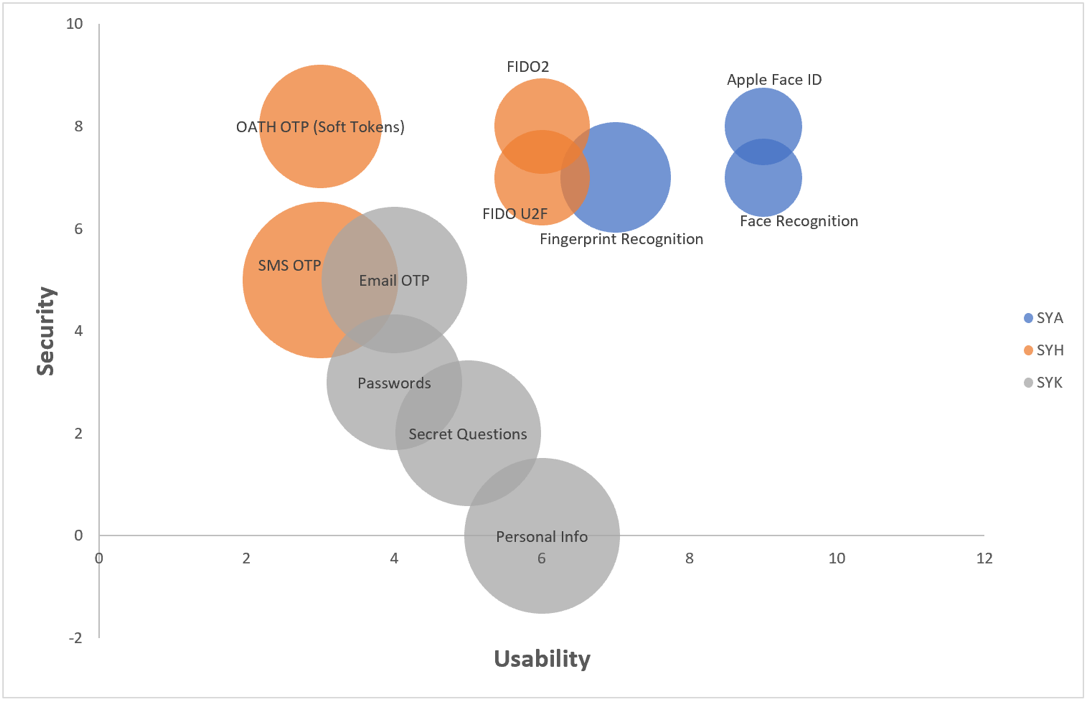
\includegraphics[width=1\linewidth]{imgs/wyk1.png}
	\caption{Porównanie metod uwierzytelniania}
	\label{fig:metody-uwierzytelniania-porownanie}
\end{figure}


\section{Sztuczne Sieci Neuronowe}
\section{Wykorzystywane narzędzia}
\subsection{Angular}
% https://vavatech.pl/technologie/frameworki/angular
% https://www.plukasiewicz.net/Angular/Angular8DataBinding

Angular jest frameworkiem do tworzenia stron internetowych typu SPA (ang. Single Page Application). Jest opracowany i rozwijany przez firmę Google. 
\paragraph{Architektura}\mbox{}\\
Podstawowym elementem architektury aplikacji Angularowych są komponenty które grupuje się, zazwyczaj ze względu na funkcjonalność, w modułach. Dzięki takiemu podejściu aplikacje są łatwo saklowalne a sama architektura przejżysta. Należy pamiętać, że wymagany jest przynajmniej jeden moduł główny w którym definiowane są najważniejsze zależności i komponenty.

\paragraph{Komponenty}\mbox{}\\
Są to pojedyncze bloki, z których zbudowana jest aplikacja napisana przy użyciu tego frameworka. Na komponent składa się zazwyczaj zestaw 3 plików składowych, z których każdy pełni określoną rolę:
\begin{itemize}
  \item Plik logiki (*.ts) --- zawierający logikę danego komponentu, w tym metody, zmienne oraz obsługę zdarzeń. W tym pliku możliwy jest import dodatkowych bibliotek lub funkcji aby rozszerzyć funkcjonalność i działanie danego komponentu 
  \item Plik szablonu (*.html) --- definiuje strukturę i wygląd komponentu. Oprócz podstawowych znaczników HTML można umieszczać w nim specjalne wbudowane lub własne dyrektywy dzięki którym można rozszerzyć funkcjonalność komponentu.
  \item Plik szablonu styli (*.css) --- służy do definicji wyglądu i formatowania komponentu zgodnie z przyjętymi założeniami projektowymi aby tworzyć estetyczne i interaktywne komponenty
\end{itemize}

\paragraph{Dekoratory klas}\mbox{}\\
Służą one do modyfikacji podstawowych klas do elementów architektury Angulara. Oprócz dekoratora \emph{@Component}, służącego do definiowania komponentu, można wyróżnić dwa dodatkowe, najbardziej podstawowe dekoratory:
\begin{itemize}
  \item @NgModule --- służy do definiowania modułu angularowego, który służy do grupowania elementów w logiczne jednostki. W modułach można między innymi deklarować komponenty, wchodzące w skład danego modułu, importować zewnętrzne moduły, aby rozszerzyć funkcjonalność oraz eksportować takie elementy, które mogą zostać wykorzystane w innym module.
  \item @Injectable --- pozwala tworzyć serwisy, usługi które mogą służyć do udostępnienia wspólnej funkcjonalności między komponentami lub częściami aplikacji
\end{itemize}

\paragraph{Powiązanie danych}\mbox{}\\
Jest to podstawowa koncepcja, która służy do komunikacji danych w komponencie i łączenia danych z widokiem. Angular oferuje wiązania jedno oraz dwukierunkowe. Wyróżnia się cztery typy wiązań:
\begin{itemize}
  \item String Interpolation --- jednokierunkowe wiązanie, którego zadaniem jest wyświetlanie danych w widoku. 
  \item Property Binding --- jednokierunkowe wiązanie, pozwala na wiązanie właściwości znaczników HTML z danymi komponentu.
  \item Event Binding --- jednokierunkowe wiązanie, które pozwala na obsługę zdarzeń wywołanych po interacji z elementami widoku
  \item Two-way binding --- dwukierunkowe wiązanie, pozwalające na wyświetlanie danych z komponentu i edycję takich danych przez użytkownika 
\end{itemize}

\begin{figure}[ht]
	\centering
		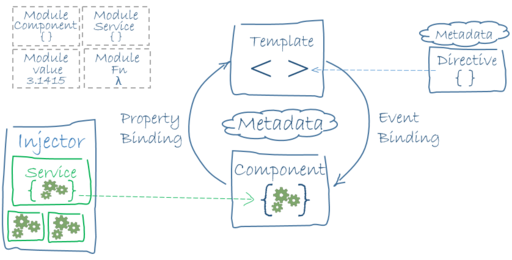
\includegraphics[width=0.6\linewidth]{imgs/ang-diag-1.png}
	\caption{Diagram powiązania elementów Angulara}
	\label{fig:wiazanie-elementow-angular}
\end{figure}

\subsection{NestJS}
% https://geek.justjoin.it/nestjs-czym-jest-jakie-ma-funkcje-jakie-sa-wady-i-zalety-tego-frameworka/
Nest JS jest frameworkiem opartym o platformę Node.JS, służącym do tworzenia aplikacji po stronie backendu z wykorzystaniem języka TypeScript. Wykorzystuje architekturę modułową, podobną do tej wykorzystywanej we frameworku Angular, dzięki czemu możliwe jest tworzenie skalowanych i wydajnych aplikacji.
\paragraph{Modułowość}\mbox{}\\
Podobnie jak we frameworku Angular, modułowość służy do grupowania elementów w logiczne jednostki. W modułach definiowane są poszczególne elementy składowe aplikacji oraz potrzebne, do poprawnego funkcjonowania, zależności.

\paragraph{Kontrolery i serwisy}\mbox{}\\
Serwisy, podobnie jak komponenty w Angularze, są pojedynczymi elementami w których zawarta jest logika biznesowa związana z konkretną funkcjonalnością. Dodatkowo w serwisach często wykonywane są podstawowe operacje CRUD bezpośrednio na modelach bazy danych. \\
Kontrolery służą do komunikacji między aplikacją kliencką a logiką biznesową z wykorzystaniem protokołu HTTP oraz podstawowych metod GET, POST, PUT, PATCH oraz DELETE.

\paragraph{Wzorce projektowe}\mbox{}\\
Nest.JS jest opracowany tak, aby można było korzystać z popularnych wzorców projektowych, takich jak wstrzykiwanie zależności oraz odwrócenie kontroli, co pozwala zapewnić lepszą strukturę i architekturę aplikacji.

\paragraph{NPM}\mbox{}\\
Z tego powodu, że Nest.JS oparty jest o platformę Node.JS to wspiera repozytorium NPM. Dzięki temu podstawowe funkcjonalności można rozszerzać o dodatkowe i często wykorzystywane biblioteki tworząc zaawansowane, biznesowe aplikacje backendowe.

\begin{figure}[ht]
	\centering
		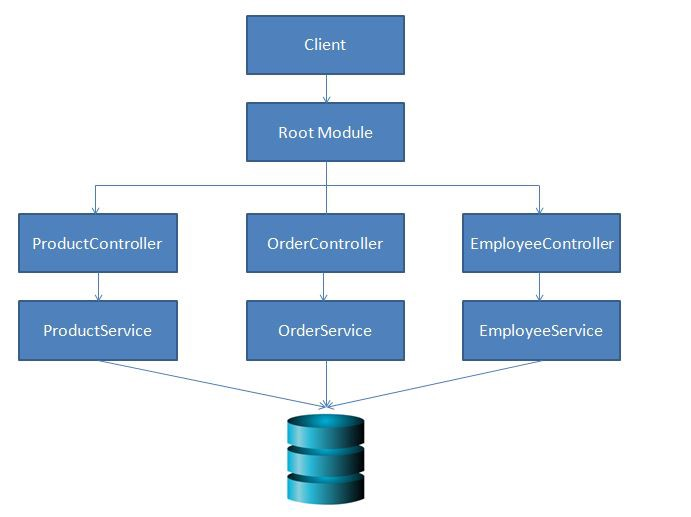
\includegraphics[width=0.6\linewidth]{imgs/nest-diag.jpeg}
	\caption{Schemat uproszczonej architektury aplikacji}
	\label{fig:nest-uproszczona-architektura}
\end{figure}

\subsection{Python}
W kręgach entuzajstów uczenia maszynowego oraz sztucznych sieci neuronowych można zauważyć dużą popularność przy wykorzystaniu języka Python do implementacji takich rozwiązań. Sam język jest wysokopoziomowym, interpretowalnym językiem programowania ogólnego przeznaczenia. Dzięki swojej czytelnej, prostej składni jest wykorzystywany w wielu dziedzinach, w tym algorytmach sztucznej inteligencji.

\paragraph{Składnia}\mbox{}\\
W przeciwieństwie do sporej liczby języków programowania, Python wykorzystuje prostą, przejrzystą składnię opartą na wcięciach. Między innymi przez swoją składnię jest wybierany jako pierwszy język do nauki programowania

\paragraph{Dynamiczne typowanie}\mbox{}\\
Programując przy użyciu tego języka można zauważyć, że zmienne lub metody nie muszą mieć określonego typu. W przeciwieństwie do innych języków, typ danych określany jest dynamicznie w trakcie wykonywania programu, dzięki czemu zyskał on dużą popularność w zakresie data science.

\paragraph{Biblioteki}\mbox{}\\
Jedną z zalet Pythona jest obszerna biblioteka standardowa, która zapewnia dostęp do różnych klas oraz funkcji. Dzięki temu na start użytkownik otrzymuje bardzo rozbudowane narzędzie programistyczne, które nadaje się do różnych zastosowań. Warto również zwrócić uwagę na rozbudowaną społeczność tego języka, która tworzy i udostępnia własne biblioteki, a część z nich stała się już obecnie standardem. Dla przykładu wiele rozwiązań z zakresu uczenia maszynowego opiera się o popularne biblioteki pokroju NumPY lub MatplotLib które ułatwiają i usprawniają pracę na danych tabelarycznych oraz pomagają wizualizować dane w różny sposób.

\subsection{MongoDB}
%https://appmaster.io/pl/blog/czym-jest-mongodb
Bazy danych są bezpośrednio związane z rozwiązaniami informatycznymi już od wielu lat. Dawniej obowiązującym standardem były relacyjne bazy jak na przykład MySQL, które były znane z powiązań relacyjnych między tabelami w bazie. Obecnie można zauważyć wzorst popularności rozwiąząń nierelacyjnych baz danych w tym MongoDB.
Jest to baza danych, w której obiekty, dane przechowywane są w postaci dokumentów, strukturą zbliżoną do obiektów JSON. Charakterystyczne dla takich baz jest brak ściśle zdefiniowanej struktury obiektów, przez co dane wchodzące w skład kolekcji moża różnić się strukturą między sobą.
Dodatkowo MongoDB jest znane z bardzo dobrej skalowalności, zarówno poziomej jak i pionowej, obsługi bardzo dużej ilości danych oraz wsparcia dla wielu języków programowania dzięki czemu bardzo łatwo jest wykorzystać tą bazę w projekcie. 

\subsection{RabbitMQ}
% https://czterytygodnie.pl/rabbitmq/wprowadzenie-do-kolejkowania-rabbitmq.html
Mówiąc o systemach mikroserwisowych warto wspomnieć o mechanizmach, które pozwalają na komunikację między poszczególnymi serwisami. Jest wiele różnych narzędzi wspierających taki proces a jednym z nich jest wykorzystanie brokera wiadomości.
Jednym z popularniejszych systemów oferujących takie rozwiązanie jest RabbitMQ. Pozwala na wysyłanie i odbieranie wiadomości przy wykorzystaniu kanałów oraz kolejek wiadomości. Wieloplatrofmowość oraz wsparcie dla wielu popularnych języków programowania sprawia, że omawiane narzędzie jest bardzo często wykorzystywane do łączenia ze sobą mikroserwisów, nawet tych napisanych przy wykorzystaniu różnych języków programwnia. Dzięki swojej skalowalności i elastyczności, RabbitMQ zyskuje popularność w wielu systemach informatycznych.


\subsection{Docker}
% https://sii.pl/blog/docker-dla-programistow-co-to-jest/?category=development-na-twardo&tag=devops,docker,kontener
Badjąc statystyki opisujące które technologie, zdaniem programistów, są najbardziej pożądane można zauważyć, że oprócz znajomości systemu kontroli wersji (git) na takim samym poziomie jest znajomość Dockera. W dobie rozwiązań chmurowych, mikroserwisowych wirtualizacja środowisk, systemów informatycznych jest niezwykle ważnym tematem ponieważ zapewnia jednolite działanie systemu bez względu na platformę na której jest uruchamiany. Dzięki solidnej realizacji tego zadania Docker zyskał niezwykłą popularność na przełomie kilku ostatnich lat 
Najprościej mówiąc, Docker jest narzędziem do wirtualizacji środowisk programistycznych, wykonawczych, które oferuje tworzenie niezależnych od siebie kontenerów. Kontener jest lekkim, samodzielnym oraz wykonywalnym pakietem oprogramowania który zawiera wszystko, co niezbędne aby dany serwis lub usługa została uruchomiona.
\subsection{Face Recognition}
% https://medium.com/@ageitgey/machine-learning-is-fun-part-4-modern-face-recognition-with-deep-learning-c3cffc121d78
W wielu serwisach i aplikacjach internetowych, oferujących publikowanie zdjęć użytkowników, wykorzystuje algorytmy do detekcji twarzy, a czasem nawet i rozpoznawanie twarzy użytkowników na zdjęciach. Do jeszcze nie tak dawna temu, narzędzia oferujące tego typu rozwiązania nie były dostępne dla początkujących programistów, a przynajmniej nie za darmo. Chcąc zaimplementować mechanizm detekcji lub rozpoznawania twarzy należało samemu opracować oraz wytrenować model sieci neuronowej. Jednak proces ten nie należy do najłatwiejszych i wymaga odpowiedniej wiedzy i doświadczenia do tego, aby stworzyć model, który ma predykcję na dobrym poziomie i \textbf{można mu ufać (#CHANGE)}.
Od niedawna dostępna jest otwartoźródłowa biblioteka dla języka Python, oferująca proces detekcji i rozpoznawaia twarzy na bardzo dobrym poziomie z dokładnością do 98\%.\\

\subsection{Xception}

% https://isolution.pl/blog/domain-adaptation-with-xception-and-vgg16-models/
% https://arxiv.org/pdf/1610.02357.pdf
\chapter{Metodologia}
\section{Platforma testowa}
Aby zbadać skuteczność rozpoznawania twarzy jako metody uwierzytelniającej użytkowników należało w pierwszej kolejności opracować oraz zaimplementować platformę testową. Dzięki niej w dalszej części pracy będzie możliwe przeprowadzenie badań z udziałem internautów.

% \subsubsection{Wymagania funkcjonalne i niefunkcjonalne}
% Proces określenia wymagań funkcjonalnych oraz niefunkcjoanlnych jest kluczowym aspektem w fazie projektowania systemu. Pozwala stworzyć pełen zbiór wytycznych związanych z funkcjonowaniem i działaniem systemu.

% \paragraph{Wymagania funkcjonalne}
% \begin{itemize}
%   \item Rejestracja użytkownika
%   \item Logowanie użytkownika przy pomocy tradycyjnej metody
%   \item Logowanie użytkownika przy pomocy rozpoznawania twarzy
%   \item Dostęp do podstawowych danych użytkownika
%   \item Wyświetlanie metryk 
% \end{itemize}

\subsubsection{Modele danych}
Kolejnym etapem w procesie projektowania systemu informatycznego jest opracowanie modelu danych. Pozwala to na wyselekcjonowanie niezbędnych danych do funkcjonowania systemu, które będą następnie wykorzystywane do tworzenia poszczególnych tabel lub kolecji danych. Dzięki temu możliwe jest skuteczne zaplanowanie struktury danych, na podstawie której będzie funkcjonował serwis. Ważnym aspektem jest fakt, że staranne opracowanie modelu danych pozwoli na minimalizację problemów na dalszych etapach tworzenia platformy testowej. Można wyróżnić 3 podstawowe modele danych: \emph{konceptualny}, \emph{logiczny} oraz \emph{fizyczny}. Ze względu na niski stopień skomplikowania systemu stworzony został tylko model fizyczny danych, dzięki któremu dalszy proces imlpementacji rzeczywistej aplikacji przebiegał sprawniej. 

% TODO
\begin{figure}[ht]
	\centering
		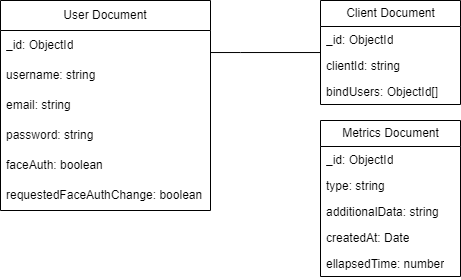
\includegraphics[width=0.5\linewidth]{imgs/db-model.png}
	\caption{Fizyczny model danych}
	\label{fig:model-danych}
\end{figure}
\subsubsection{Architektura aplikacji}
\begin{figure}[ht]
	\centering
		\includegraphics[width=1\linewidth]{imgs/Diagram bez tytułu.drawio (2).png}
	\caption{Architektura platformy testowej}
	\label{fig:architektura-aplikacji}
\end{figure}

Obecnie istnieje kilka popularnych architektur, które wykorzystywane są do budowy aplikacji internetowych. W etapie projektowania platformy zdecydowano się na wykorzystanie architektury mikroserwisowej wykorzystującej kolejkę wiadomości do komunikacji między pomniejszymi serwisami. Na początku warto zaznaczyć, że mikroserwisy cechują się bardzo dobrą skalowalnością, wykrywaniem oraz naprawianiem potencjalnych błędów w oprogramowaniu. Z uwagi na fakt wykorzystywania różnych języków programowania przy implementacji aplikacji serwerowej, wykorzystanie takiej architektury było bardzo dobrym rozwiązaniem, zapewniającym integrację serwisów na wysokim poziomie.
Analizując diagram przedstawiony na rysunku 3.1 można wyróżnić 3 główne warstwy.

\paragraph{Warstwa dostępowa} zadaniem której jest komunikacja serwisu z użytkownikiem, wykorzystując aplikację napisaną przy użyciu frameworka Angular. Przy pomocy tej warstwy użytkownik może przetestować różne metody uwierzytelniania w tym logowanie przy pomocy rozpoznawania twarzy.

\paragraph{Warstwa biznesowa} Jej zadaniem jest przetwarzanie danych otrzymanych z aplikacji dostępowej. W jej skład wchodzi kilka niezbędnych składników:
\begin{itemize}
  \item Gateway --- służy jako bramka, do oddelegowania zapytań użytkownika na określone serwisy przy pomocy kolejki wiadomości
  \item Kolejka wiadomości --- jej zadaniem jest wymiana wiadomości między dostępnymi mikroserwisami
  \item UserApp --- serwis do zarządzania użytkownikami. W jego skład wchodzą metody odpowiedzialne za tworzenie oraz pobieranie niezbędnych danych użytkowników
  \item AuthApp --- serwis zarządzający uwierzytelnianiem użytkowników zarówno tradycyjnymi metodami jak i metodami wykorzystującymi sztuczną inteligencję.
  \item ClientApp --- serwis, którego głównym zadaniem jest rejestracja urządzeń z których użytkownik się loguje do zapewnienia większego bezpieczeństwa płynącego z wykorzystania rozpoznawania twarzy.
  \item MetricsApp --- serwis który zbiera dane o czasie wykonywania procesu logowania różnymi metodami.
  \item AIApp --- serwis którego zadaniem jest przetwarzanie zdjęć użytkowników oraz udostępnianie metod do rozpoznawania twarzy.
\end{itemize}

\paragraph{Warstwa danych} Służy do przechowywania danych serwisu oraz wykonywanie operacji na bazie danych. Wykorzysuje MongoDB.
\\
Aby umożliwić uruchomienie aplikacji na dedykowanym serwerze, niezbędne było wykorzystanie narzędzia Docker. Umożliwiło to stworzenie oddzielnego środowiska wykonawczego w postaci osobnych kontenerów na każdy z utworzonych serwisów, w tym bazy danych oraz kolejki wiadomości, który mógł zostać uruchomiony na dowolnej platformie. Aby zapewnić większe bezpieczeństwo aplikacji oraz urchonić mikroserwisy przed nieuprawnionym dostępem, poszczególne aplikacje komunikują się poprzez wykorzystanie wewnętrznej sieci między kontenerami. Udostępnione zostały 2 porty, z którymi komunikować mogła się aplikacja dostępowa:
\begin{itemize}
  \item \emph{\:5000} --- port, na którym udostepniony jest serwis związany z wykorzystaniem sztucznej inteligencji do rozpoznawania twarzy
  \item \emph{\:9000} --- port, na którym udostępniona jest bramka, która oddelegowuje odpowiednie rządania poprzez kolejkę wiadomości do odpowiednich serwisów.
\end{itemize}

\subsubsection{Widoki}
Frontend platformy testowej składa się z dwóch głównych widoków oraz szeregu funkcjonalności dzięki którym mozliwe jest przetestowanie tradycyjnych metod logowania z tymi wykorzystującymi rozpoznawanie twarzy. \\
\textbf{Strona logowania} na której użytkownik może:
\begin{itemize}
   \item stworzyć nowe konto --- podając kluczowe do działania apllikacji dane oraz dodatkowo zeskanować twarz jeżeli użytkownik wyraził chęć logowania przy pomocy rozpoznawania twarzy
   \item zalogować się na konto --- wybierając jedną z dostępnych metod czyli tradycyjne logowanie hasłem oraz logowanie rozpoznawaniem twarzy z wyborem który algorytm ma zaostać wykorzystany.
\end{itemize}

\textbf{Strona panelu użtkownika} oferująca:
\begin{itemize}
  \item przeglądanie danych użytkownika --- zarówno tych podanych w procesie rejestracji jak i dodatkowe dane takie, jak zapisane przeglądarki.
  \item wylogowanie z systemu
  \item przeglądanie danych logowania --- lista danych o procesach logowania w skład których wchodzi czas oraz informacja na temat wybranej metody logowania.
\end{itemize}

% \subsubsection{Opis API}
% W serwisach internetowych obowiązującym standardem komunikacji jest protoków HTTP (ang. Hyper Text Transfer Protocol). Wykorzystuje się go do komunikacji między warstwą dostępową a warstwą biznesową, która udostępnia API (ang. Application Programming Interface). W przypadku omawianej platformy testowej można wyróżnić:
% \begin{itemize}
%   \item \emph{POST :9000/api/v1/gateway/auth/login} --- logowanie hasłowe
%   \item \emph{POST :9000/api/v1/gateway/auth/face-login} --- logowanie twarzą
%   \item \emph{POST :9000/api/v1/gateway/client/register} --- logowanie
%   \item \emph{POST :9000/api/v1/gateway/client/bind} --- logowanie
%   \item \emph{POST :9000/api/v1/gateway/client/unbind} --- logowanie
%   \item \emph{POST :9000/api/v1/gateway/auth/login} --- logowanie

% \end{itemize}

\subsubsection{Zabezpieczenia}
\paragraph{JSON Web Token} standard wymiany tokenów, zapewniający warstwę zabezpieczającą przed nieautoryzowanym dostępem do aplikacji. JWT został wykorzystany, jako kluczowy element potwierdzający, że dany użytkownik zalogował się poprawnymi danymi do systemu. Działanie mechanizmu rozpoczyna się od wykonania akcji, mającej na celu zalogowanie uzytkownika, zarówno tradycyjną metodą jak i przy pomocy rozpoznawania twarzy. W przypadku, kiedy system potwierdzi wiarygodność danego użytkownika, następuje wygenerowanie tokenu przy pomocy algorytmów kryptograficznych. Opcjonalnie można podać dane, które zostaną zapisane do takiego unikalnego tokena. Ostatnim krokiem jest wysłanie go do aplikacji dostępowej i zapisanie w pamięci przeglądarki. Sam token składa się z 3 elementów:
\begin{itemize}
  \item Header - zawiera typ tokena oraz algorytm szyfrujący
  \item Payload - zazwyczaj zawiera opcjonalne dane, zapisane programistycznie oraz długość życia tokenu
  \item Verify - podpis cyfrowy stanowiący sumę kontrolną do weryfikacji poprawności tokenu
\end{itemize}

\paragraph{Zapisywanie przeglądarki} ma na celu uniemożliwienie logowania przy pomocy rozpoznawania twarzy na urządzeniach niezaufanych. Algorytmy i sieci neuronowe, których zadaniem jest rozpoznwanie twarzy same w sobie nie są w żaden sposób zabezpieczone na różne ataki. Przykładem może być próba logowania przy pomocy zdjęcia dowolnego użytkownika, który zarejestrowany jest w systemie. Jednym z proszych w imlpementacji zabezpieczeń jest wykorzystanie zapamiętywania urządzenia (przeglądarki) użytkownika. Dzięki czemu opcja logowania przy pomocy rozpoznawania twarzy jest możliwa tylko na zaufanych urządzeniach. Sposobem na dodanie zaufanej przeglądarki jest zarejestrowanie lub zalogowanie tradycyjną metodą.


\section{Model sieci neuronowej}
\subsubsection{Dane}
Wybór odpowiedniego zbioru danych jest kluczowym elementem w procesie uczenia oraz testowania opracowanych modeli uczenia głębiokiego. Na potrzeby niniejszej pracy wykorzystany został gotowy zbiór danych \emph{CelebA Face Recognition Triplets} opracowany przez [...]. Zbiór danych składa się z pliku .csv który zawiera 16000 trójek zdjęć - Anchor, Positive, Negative oraz 45000 zdjęć twary różnych osób. Wykorzystanie gotowego zbioru danych pozwoliło zaoszczędzić czas na ręczne dobieranie i walidowanie zdjęć twarzy.
Każde zdjęcie w omawianym zbiorze ma rozmiar 224px na 224px oraz składa się z 3 kanałów kolorystycznych (R,G,B).
\subsubsection{Architektura sieci}
Opracowany model sieci jest siecią typu syjamskiego. Oznacza to, że do działania wykorzystuje 2 lub więcej identycznych podsieci uczenia głębokiego, do realizowania zadania. Takie sieci nie służą do klasyfikacji lub etykietowania zdjęć. Zazwyczaj służą do obliczania dystansu (podobieństwa) między parami zdjęć. Dlatego też tego typu sieci doskonale nadają się do realizowania zadania rozpoznawania twarzy. \\
Opracowana syjamska sieć neuronowa wykorzystuje model Xception w swoich podsieciach. Aby przyspieszyć proces implementacji, wykorzystano gotowy, wytrenowany model tej sieci z biblioteki Keras. Celem sieci Xception jest konwersja zdjęcia twarzy na postać wektorową która jest wykorzystywana na późniejszym etapie rozpoznawania twarzy.
Danymi wejściowymi dla głównej sieci są trójki zdjęć - referencyjne, pozytywne to jest takie które predstawia tą samą osobę co na zdjęciu referencyjnym, oraz negatywne przedstawiająće zupełnie inną osobę. Trójki zdjęć w późniejszym etapie są rozdzielane na korespondujące im gałęzie sieci, aby przekonwertować je na postać numeryczną. Zbiór 3 wektorów trafia do warstwy dystansu, w której obliczana jest odległość między zdjęciem referencyjnym a negatywnym oraz pozytywnym. 
\subsubsection{Miary Ocen}
Miarą oceny skuteczności opracowanego modelu jest funkcja potrójnej straty wykorzystywana w warstwie dystansu.
$$ L(a, p, n) = max(d(a, p) - d(a, n) + \alpha, 0) $$
  Jej zadaniem jest minimalizacja różnicy odległości między referencyjnym a pozytywnym wektorem cech oraz maksymalizacja dystansu między referencyjnym a negatywnym wektorem cech. Celem tej funkcji jest zapewnienie aby pozytywne wektory cech były osadzone bliżej a negatywne wektory dalej referencyjnego wektora. Dzięki temu model powinien skuteczniej weryfikować, czy dwa zdjęcia twarzy należą do tej samej osoby.
Funkcja przyjmuje 4 parametry:
\begin{itemize}
  \item a, \emph{anchor} --- wektor cech zdjęcia referencyjnego danej osoby
  \item p, \emph{positive} --- wektor cech zdjęcia przedstawiającego tą samą osobę co na zdjęciu referencyjnym
  \item n, \emph{negative} --- wektor cech zdjęcia przedstawiającego inną osobę
  \item $\alpha$ --- margines
\end{itemize}
Na ich podstawie obliczana jest różnica odległości euklidesowych między wektorem referencyjnym i pozytywnym oraz wektorem referencyjnym i negatywnym. Do takiej różnicy dodawany jest margines, którego zadaniem jest kontrola minimalnej różnicy między odległościami. Ostatecznym wynikiem funkcji jest maskymalna wartość miedzy wartością obliczoną na podstawie danych parametrów a liczbą 0. 
\subsubsection{Proces uczenia}
Pierwszym etapem w procesie uczenia było rozbicie danych na zbiór trenujący oraz testujący w proporcji 80\% dla uczącego oraz 20\% dla walidującego. \\
Dla polepszenia wyników uczenia, wykorzystane zostały generatory zdjęć na podstawie utworzonych wcześniej zbiorów. Zadaniem generatorów obrazów jest augmentacja, czyli dynamiczne modyfikowanie zdjęć poprzez ich obracanie, skalowanie lub przesuwanie w czasie rzeczywistym. Augmentacja zdjęć zbioru uczącego wpływa na skuteczność nauki modelu sieci neuronowej oraz zapobiega przetrenowaniu modelu. Biblioteka Tensorflow oferuje gotowe rozwiązania implementacyjne takich generatorów danych. \\
Podczas kompilowania sieci wykorzystano optymalizator Adam o parametrach learning\_rate = 0,001, epsilon=0,1. Tego typu optymalizator jest powszechnie używany ze względu na jego właściwości adaptacyjne do różnych typów danych i problemów a także na prostotę w implementacji. Współczynnik nauki determinuje wielkość kroku aktualizacji wag a parametr epsilon ma zapobiegać dzieleniu przez zero przy oblicznaiu wartości wagi. \\
W procesie uczenia wykorzystsano kilka dodatkowych mechanik, których zadaniem jest zwiększenie efektywności nauki oraz zapobieganiu przetrenowania sieci.
\paragraph{ModelCheckpoint} --- Callback mający za zadanie na bieżąco zapisywać najlepsze wagi modelu do pliku na podstawie przekazanej metryki. Po każdej epoce sprawdzana jest wartość metryki, a wagi są zapisywane w momencie kiedy wartość metryki osiągnęła rządaną wartość, zazwyczaj mniejszą lub większą niż w epoce dotychczas najlepszej.  
\paragraph{EarlyStopping} --- Callback służący do przerywania procesu uczenia w momencie, kiedy jakoś modelu mierzona wybraną, przekazaną metryką, nie poprawiła się. Dodatkowo do tej metody można przekazać parametr patience, którego zadaniem jest przeczekanie danej liczby epok i przerwanie procesu pod warunkiem, że jakoś modelu się nie poprawiła.
\paragraph{ReduceLROnPlateu} --- Callback który obniża współczynnik nauki w momencie kiedy jakość modelu się nie poprawiła po n-liczbie epok. Przyjmuje takie parametry, jak patience, określające po ilu epokach ma obniżyć wpółczynnik, factor, określający o ile ma się mniejszyć learning\_rate, oraz min\_lr, który określa minimalną granicę.
Kolejnym krokiem było uruchomienie procesu uczenia o zadanych parametrach:
\begin{itemize}
  \item Liczba Epok - 250
  \item Batch - 32
  \item Rozmiar zdjęć - 225x225px
\end{itemize}
\begin{lstlisting}
  history = siameseModel.fit(
    train_generator, validation_data=test_generator, epochs=EPOCHS, callbacks=[
      checkpoint, earlystop, learning_rate_reduction
    ]
  )
\end{lstlisting}
Dane o procesie uczenia zostały dodatkowo zapisane do zmiennej \emph{history}, dzięki czemu możliwa była dalsza analiza wyników po zakończonym procesie. Wykorzystując bibliotekę \emph{matplotlib} wygenerowane zostały wykresy metryk modelu. Dodatkowo wagi modelu zostały zapisane do pliku, dzięki czemu możliwe było wykorzystanie wyuczonego modelu w platformie testowej do dalszej analizy

\subsubsection{Ocena modelu}
Model był oceniany z wykorzystaniem miar:
\paragraph{Validation Loss} obliczana na podsatwie funkcji potrójnej straty na zbiorze walidującym. Określa jak bardzo predykcja modelu różni się od rzeczywistych danych. Jej wartość powinna się minimalizować wraz z postępem uczenia sieci.

% \begin{figure}[ht]
% 	\centering
% 		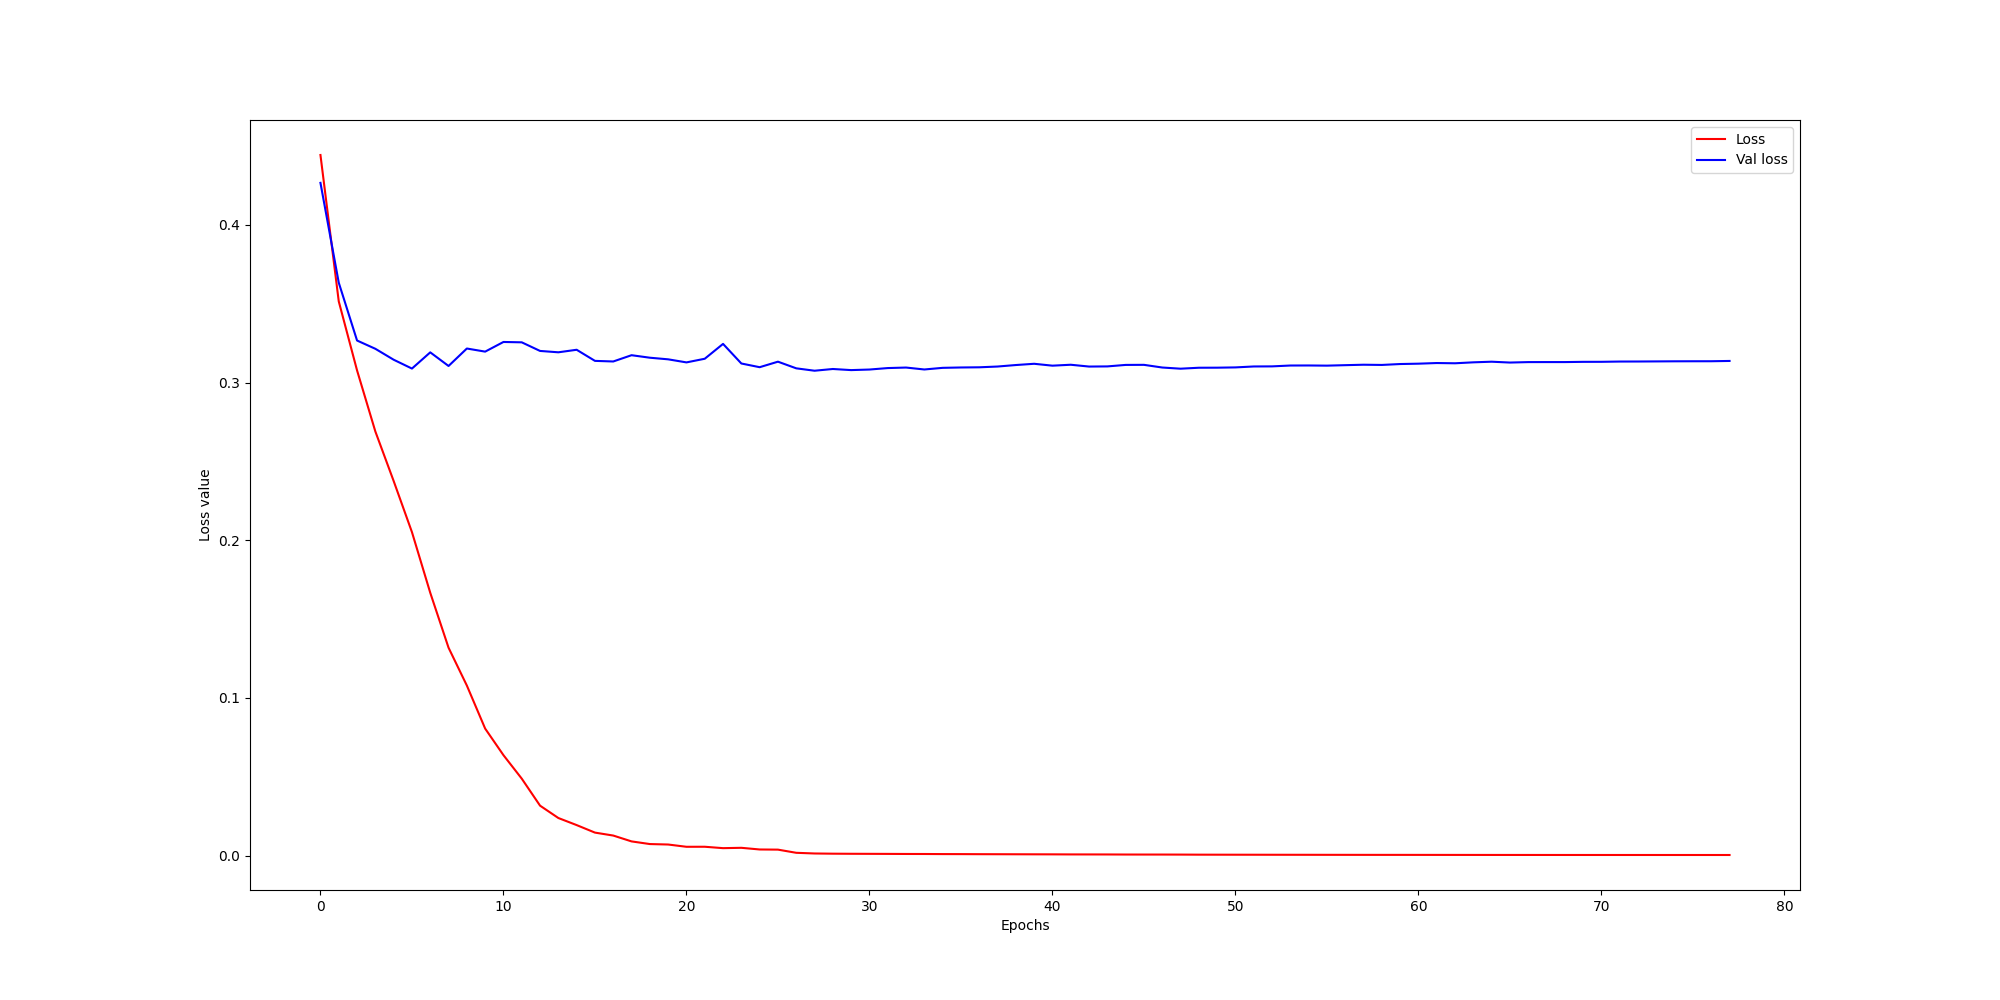
\includegraphics[width=1\linewidth]{imgs/training-76-epochs.png}
% 	\caption{Wykres uczenia}
% 	\label{fig:ucznenie}
% \end{figure}

\paragraph{Accuracy} obliczana na późniejszym etapie przy ewaluacji modelu na różnych zbiorach danych na podstawie wzoru:
$$ acc = \frac{true\_predictions}{total} $$ 

% \begin{figure}[htb]
%   \centering
% 	\begin{tabular}{@{}ll@{}}
% 	a) & b) \\
%   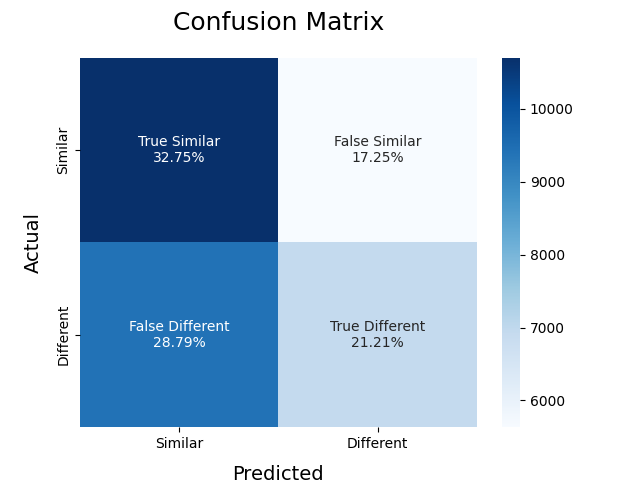
\includegraphics[width=0.475\textwidth]{imgs/celeba-learning-acc=0.5396154788145971.png} & 
% 	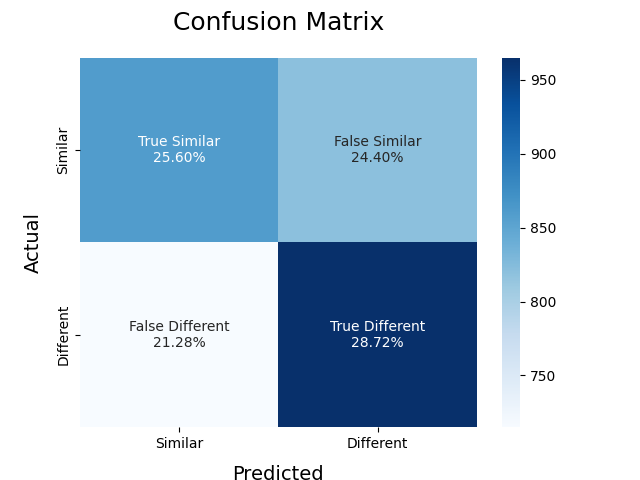
\includegraphics[width=0.475\textwidth]{imgs/lfw-learning-acc=0.5431547619047619.png}
% 	% jeśli obraki są różnej wysokości, można je wyrównać do góry stosując vtop jak niżej
% 	% \vtop{\vskip-2ex\hbox{{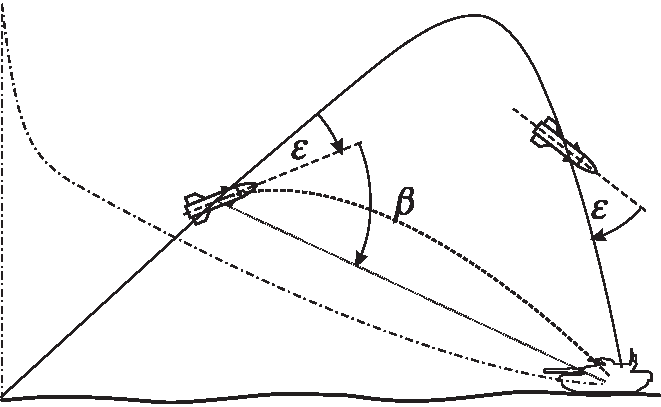
\includegraphics[width=0.475\textwidth]{rys05/beta1}}}} &
% 	% \vtop{\vskip-2ex\hbox{{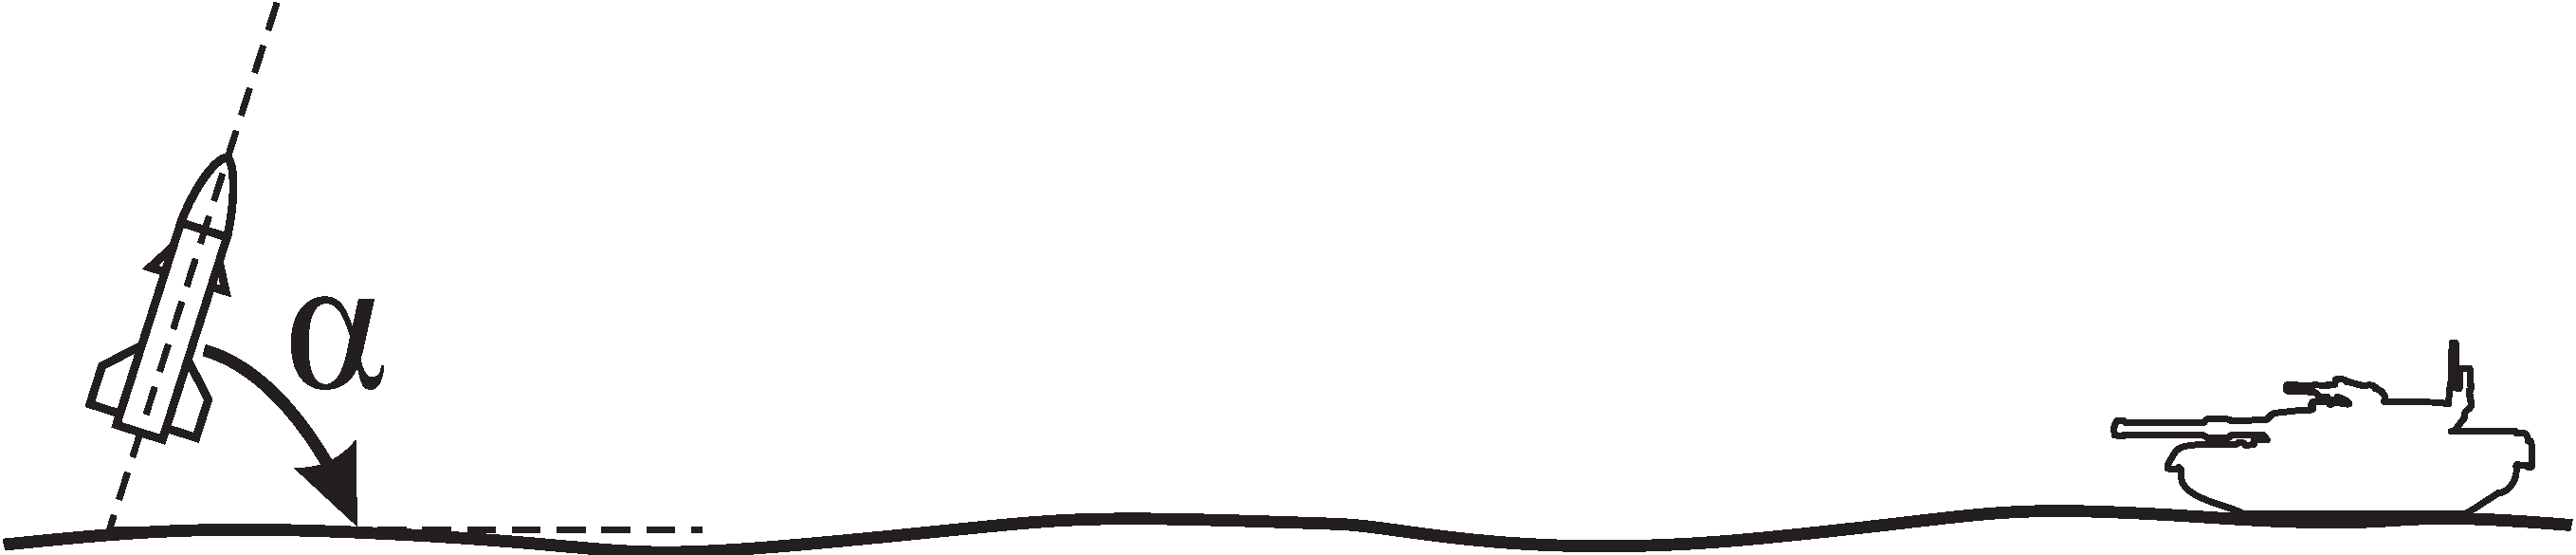
\includegraphics[width=0.475\textwidth]{rys05/alfa1}}}}  \caption{Wyznaczanie trajektorii lotu rakiety: 
% 	\end{tabular}
%   \caption{Macierz konfuzji: a) Dla zbioru CelebA, b) Dla zbioru LFW}
%   \label{fig:conf}
% \end{figure}

% Przy pomocy metryk wyznaczono, że model ma 53\% dokładność przy jednoczesnej wartości straty walidacyjnej na poziomie 0,3. Oznacza to, że model jest w dobrym stopniu dopasowany do danych walidacyjnych ale ma dokładność na niskim poziomie.

\section{Opracowanie ankiety}
Zadaniem ankiety było zbadanie doświadczeń i opinii osób na temat metod uwierzytelniania w tym takich, które wykorzystują sztuczną inteligencję. Grupa badawcza składała się z przypadkowych osób z różnych grup wiekowych o zróżnicowanym doświadczeniu z aplikacjiami internetowymi aby wyniki były obiektywne oraz zróżnicowane pod kątem opinii oraz doświadczeń. \\
Ankieta została opracowana przy pomocy aplikacji \emph{Microsoft Forms}, które jest bardzo popularnym i darmowym narzędziem do tworzenia ankiet. Oferuje możliwość personalizacji oraz tworzenia bardzo zaawansowanych kwestionariuszy pod kątem różnych typów odpowiedzi użytkowników. Dodatkowo aplikacja oferuje podgląd zebranych odpowiedzi oraz prezentację wyników w postaci rożnego rodzaju wykresów co na etapie analizy jest bardzo pomocne
\subsection{Doświadczenia z metodami uwierzytelniania i sztuczną inteligencją} Pierwsza część ankiety skupiała się na zbadaniu doświadczenia użytkowników z powszechnie dostępnymi metodami uwierzytelniania oraz ich bezpieczeństwem. Ponadto ta część miała również za zadanie zebranie danych na temat odczuć grupy badawczej na temat wykorzystania sztucznej inteligencji w zakresie bezpieczeństwa w internecie.

\begin{table}[htb]
\centering
\caption{Zbiór pytań pierwszej części ankiety}
\label{tab:ankieta-part-1}\small
\begin{tabularx}{\linewidth}{|c|X|X|} 
  \hline
Nr & Pytanie & Typ \\ 
\hline\hline
1 & Grupa wiekowa do której należysz & Jednokrotny wybór \\
2 & Ile godzin spędzasz w internecie? & Jednokrotny wybór \\
3 & Jakie urządzenie wykorzystujesz najczęściej do przebywania w internecie & Wielokrotny wybór \\
4 & Jakie jest Twoje doświadczenie z metodami uwierzytelniania & Ocena 1-5 \\
5 & W której dziedzinie najczęściej wykorzystujesz metody uwierzytelniania & Jednokrotny wybór \\
6 & Jakie metody uwierzytelniania stosujesz na codzień? & Wielokrotny wybór \\
7 & Oceń poniższe metody uwierzytelniania & Linkieta \\
8 & Czy padłeś/padłaś ofiarą włamania na konto & Tak/Nie \\
9 & W jaki sposób wykradziono Ci dane do logowania & Jednokrotny wybór \\
10 & Jaką metodę uwierzytelniania stosowałeś/stosowałaś wtedy? & Jednokrotny Wybór \\
11 & Jaki jest Twój stosunek do polityki haseł? & Ocena 1-5 \\
12 & Czy Twoim zdaniem polityka haseł ma znaczący wpływ na bezpieczeństwo? & Tak/Nie \\
13 & Dlaczego tak uważasz? & Odpowiedz tekstowa \\
14 & Czy zdarza Ci się czasem zapomnieć hasło? & Tak/Nie \\
15 & Jak często zdarza Ci się zapomnieć hasło? & Jednokrotny wybór \\
16 & Czy wykorzystanie sztucznej inteligencji jako metody uwierzytelniania mogłoby poprawić bezpieczeństwo? & Tak/Nie \\
17 & Dlaczego tak uważasz? & Odpowiedź tekstowa \\
18 & Czy mając możliwość stosowania uwierzytelniania przy pomocy rozpoznawania twarzy w aplikacjach internetowych wykorzystał/a byś taką opcję? & Tak/Nie \\
19 & Dlaczego? & Wypowiedź tekstowa \\
20 & Co Twoim zdaniem mogłoby poprawić bezpieczeństwo związane z metodami uwierzytelniania w aplikacjach internetowych? & Odpowiedź tekstowa \\
\hline
\end{tabularx}
\end{table}

\newpage
\subsection{Opinia z użytkowania platformy testowej} Druga część ankiety była odpowiedzialna za uzyskanie opinii grupy badawczej na temat zaproponowanych metod uwierzytelniania, tych tradycyjnych oraz wykorzystujących sztuczną inteligencję z zakresu rozpoznawania twarzy. Ocenie zostały poddane zarówno kwestie bezpieczeństwa oraz intuicyjność aplikacji.

\begin{table}[htb]
  \centering
  \caption{Zbiór pytań drugiej części ankiety}
  \label{tab:ankieta-part-2}\small
  \begin{tabularx}{\linewidth}{|c|X|X|} 
    \hline
  Nr & Pytanie & Typ \\ 
  \hline\hline
  1 & Czy miałeś/aś możliwość przetestować aplikację? & Tak/Nie\\
  2 & Czy Twoim zdaniem aplikacja jest bezpieczna & Tak/Nie \\
  3 & Czy wykorzystałeś/aś wszystkie dostępne metody uwierzytelniania? & Tak/Nie  \\
  4 & Oceń bezpieczeństwo zaprezentowanych metod uwierzytelniania & Linkieta \\
  5 & Co Twoim zdaniem mogłoby poprawić bezpieczeństwo aplikacji? & Odpowiedź tekstowa \\
  6 & Czy aplikacja była intuicyjna w obsłudze? & Tak/Nie \\
  7 & Co sprawiło że aplikacja była nieintuicyjna? & Odpowiedź tekstowa \\
  8 & Na jakim urządzeniu używałeś/aś aplikacji? & Jednokrotny wybór \\
  9 & Jakie masz uwagi co zaprezentowanej aplikacji? & Odpowiedź tekstowa \\
  \hline
  \end{tabularx}
  \end{table}
% \begin{enumerate}
  % \item Doświadczenia z metodami uwierzytelniania --- Składająca się z 20 pytań. 
  % \item Opinia po obsłudze platformy testowej --- Składająca sie z 9 pytań
% \end{enumerate}

% \chapter{Zalecenia dotyczące formatowania}
% Większa część niniejszego rozdziału ma charakter informacyjny. Treści w nim zawarte mają uzmysłowić czytelnikowi, jak wiele jest parametrów do ustawienia, by zredagowany dokument wyglądał ,,ładnie''. Parametry te poustawiano w szablonie. Wystarczy z niego skorzystać.

% \section{Rozmiar i układ treści na stronach dokumentu}
% Praca dyplomowa powinna być przygotowana do wydruku na papierze formatu A4 w orientacji pionowej.
% Marginesy na stronach parzystych i nieparzystych powinny być jednakowe i mieć następujące wartości:
% lewy = 25mm, prawy = 25mm, górny = 10mm, dolny = 15mm. Wielkość marginesów w szablonie sterowana jest parametrami przedstawionymi na rysunku~\ref{fig:pageLayout}. Margines dolny powinien być mierzony do linii bazowej tekstu stopki.
% %\begin{figure}[htb]
% 	%\centering
% 	%\includegraphics[width=.7\linewidth]{rys03/pageLayout2}
% 	%\caption{Kontrola marginesów i odstępów elementów na stronie} \label{fig:pageLayout}
% %\end{figure}
% \begin{figure}[htb]
% \setlayoutscale{0.43}
% \currentpage
% \drawparameterstrue
% %\drawpage
% \oddpagelayoutfalse
% \drawstock
% \caption{Układ strony nieparzystej dla dokumentu klasy \texttt{memoir}} \label{fig:pageLayout}
% \end{figure}

% Rzeczywisty układ strony zastosowany w niniejszym dokumencie przedstawiono na rysunku~\ref{fig:currentPageLayout}. Lewy i prawy margines są takie same, więc strony parzyste i nieparzyste wyglądają podobnie, z dokładnością do umiejscowienia notatek marginesowych. Taki rezultat zapewniło zastosowanie poniższych komend. 
% \begin{figure}[t]
% \setlayoutscale{0.43}
% \currentstock
% \oddpagelayouttrue
% \twocolumnlayoutfalse
% \drawmarginparstrue
% \drawparametersfalse
% \drawstock
% \caption{Rzeczywisty układ strony nieparzystej w tym dokumencie} \label{fig:currentPageLayout}
% \end{figure}

% \begin{lstlisting}[basicstyle=\footnotesize\ttfamily]
% \setlength{\headsep}{10pt} 
% \setlength{\headheight}{13.6pt} 
% \setlength{\footskip}{\headsep+\headheight}
% \setlength{\uppermargin}{\headheight+\headsep+1cm}
% \setlength{\textheight}{\paperheight-\uppermargin-\footskip-1.5cm}
% \setlength{\textwidth}{\paperwidth-5cm}
% \setlength{\spinemargin}{2.5cm}
% \setlength{\foremargin}{2.5cm}
% \setlength{\marginparsep}{2mm}
% \setlength{\marginparwidth}{2.3mm}
% \checkandfixthelayout[fixed] 
% \linespread{1}
% \setlength{\parindent}{14.5pt}
% \end{lstlisting}


% \section{Strona tytułowa}
% Stronę tytułową przygotowano starając się wypełnić zalecenia zamieszczone na stronie Wydziału Informatyki i Teleinformatyki (\url{https://wit.pwr.edu.pl/studenci/dyplomanci/praca-dyplomowa}, [dostęp dnia 16.12.2022]). Zastosowano więc pakiet \texttt{ebgaramond}. Dostarcza on klonu wymaganej czcionki \texttt{garamond}, jednak bez kształtu \texttt{slanted} i z pewnymi brakami. Na przykład zamiast literki ,,ł'' w zbiorze \texttt{EBGaramond08 Italic} renderuje się samo ,,l'' (braku tego nie ma zbiór \texttt{EBGaramond12}).  Zaletą pakietu  w porównaniu do innych jest to, że generalnie dobrze obsługiwane są w nim polskie znaki oraz że pakiet ten można znaleźć w różnych dystrybucjach latexa (\texttt{MikTeX} instaluje go automatycznie).

% Wielkości znaków użytych do wypełnienia strony tytułowej treścią są następujące:
% \begin{lstlisting}[basicstyle=\footnotesize\ttfamily]
% Politechnika Wrocławska (Garamond Bold 20pt 22pt)
% Wydział Informatyki i Teleinformatyki (Garamond Bold 16pt 18pt)
% Kierunek: Jakiś kierunek (Garamond 14pt 16pt, Garamond Bold 14pt 16pt)
% Specjalność: Jakaś specjalność (Garamond 14pt 16pt, Garamond Bold 14pt 16pt)
% {P}RACA {D}YPLOMOWA (Garamond 26pt 28pt, Garamond 24pt 26pt)
% {I}NŻYNIERSKA (Garamond 26pt 28pt, Garamond 24pt 26pt)
% Tytuł pracy w języku polskim (Garamond Bold 18pt 20pt)
% Title in English (Garamond Bold 18pt 20pt)
% % AUTOR: (Garamond 16pt 18pt) - zamarkowane
% Imię Nazwisko (Garamond Bold 16pt 18pt)
% Opiekun pracy (Garamond 14pt 16pt)
% tytuł/stopień naukowy, Imię Nazwisko (Garamond 14pt 16pt)
% %OCENA PRACY: (Garamond 16pt 18pt) - zamarkowane
% WROCŁAW, 2021 (Garamond 14pt 16pt)
% \end{lstlisting}


% \section{Główny tekst}
% Główny tekst pracy powinien być zredagowany z wykorzystaniem czcionki \texttt{Times}, typ normalny, o wysokości 12pt, z odstępem między liniami równym 14.5pt. Istnieje możliwość zmiany odstępu między liniami za pomocą komendy \verb?\linespread?, jednak zaleca się pozostawienie tego odstępu jak w niniejszym dokumencie (\verb?\linespread{1}?). Wymagania odnośnie kroju pisma pozostałych elementów (nagłówków, stopek itp.) zamieszczono w tabeli~\ref{tab:secfonts}.

% W szablonie zastosowano czcionkę \texttt{texgyre-termes} (dostarcza ją pakiet \texttt{tgtermes}). Czcionka ta jest klonem czcionki \texttt{Times}, w którym obsługiwane jest środkowoeuropejskie kodowanie znaków (podobnie jak w przypadku czcionki \texttt{ebgaramond}, dzięki czemu polskie literki nie są zlepkami dwóch znaków lecz pojedynczymi znakami).  

% Wszelkie przykłady źródeł kodu (fragmenty programów, komendy linii poleceń), nazwy plików i uruchamianych programów powinny być pisane czcionką maszynową. W szablonie czcionką maszynową jest \texttt{t1xtt}. Czcionka ta obsługuje polskie znaki. Dostarcza ją pakiet \texttt{txfonts}, który należy wcześniej zainstalować (MiKTeX zainstaluje go automatycznie podczas pierwszej kompilacji szablonu).   

% % https://en.wikibooks.org/wiki/LaTeX/Lengths
% % there are two different point sizes.  A pdf point is 1/72 inch.  A LaTeX point is 1/72.27 inch.  Thus,
% % the LaTeX point is slightly smaller than a pdf point. 

% %\texttt{baselineskip}: \printlength{\baselineskip}\\
% %\texttt{beforesecskip}: \printlength{\beforesecskip}\\
% %\texttt{aftersecskip}: \printlength{\aftersecskip}\\
% %\texttt{topskip}: \printlength{\topskip}\\
% %\texttt{fontsize}: \showFontSize\\

% \begin{table}[htb]
% \centering
% \caption{Zestawienie czcionek elementów podziału dokumentu, tekstu wiodącego, nagłówka i stopki oraz podpisów (Rozm. -- rozmiar czcionki, Odst. -- \texttt{baselineskip})}
% \label{tab:secfonts}\small
% \begin{tabularx}{\linewidth}{|ll@{\hskip 5pt}l@{\hskip 5pt}lX|} \hline
% Element & Przykład & Czcionka & Rozm. & Odst. \\ \hline\hline
% Nr rozdziału & {\huge\bfseries Rozdział 1 } & \verb?\huge\bfseries? & 25pt & 30pt \\
% Tytuł rozdziału & {\Huge\bfseries Wstęp } & \verb?\Huge\bfseries? & 30pt & 37pt\\
% Nr i tytuł sekcji & {\Large\bfseries 1.1. Wprowadzenie } & \verb?\Large\bfseries? & 17pt & 22pt \\
% Nr i tytuł podsekcji & {\large\bfseries 1.1.1. Cel szczegółowy } & \verb?\large\bfseries? &14.5pt & 18pt\\
% Tytuł podpodsekcji  & {\normalsize\bfseries Założenia } & \verb?\normalsize\bfseries? & 12pt & 14.5pt\\
% Tytuł paragrafu & {\normalsize\bfseries  Podstawy } Opis ... &  \verb?\normalsize\bfseries? & 12pt & 14.5pt\\
% Tekst wiodący & {\normalsize Niniejszy dokument ... } & \verb?\normalsize? & 12pt & 14.5pt\\
% Nagłówek strony & {\small\itshape 3.2. Czcionka wiodąca ...} & \verb?\small\itshape? & 11pt & 13.6pt \\
% Stopka strony & {\small Imię Nazwisko: ...} & \verb?\small? & 11pt & 13.6pt\\
% Podpisy tabel & {\small Tab.~3.1: Zestawienie ...} & \verb?\small? & 11pt & 13.6pt \\
% Podpisy rysunków & {\small Rys.~3.1: Oficjalny ...} & \verb?\small? & 11pt & 13.6pt\\\hline
% \end{tabularx}
% \end{table}
% %\texttt{fontsize}: \showFontSize

% Jeśli w pracy zostaną użyte otoczenia matematyczne, to w dokumencie wynikowym pojawią się dodatkowe czcionki (domyślne latexowe czcionki do wyrażeń matematycznych). Dzięki zastosowaniu opcji \texttt{extrafontsizes} w klasie \texttt{memoir} nie dość, że otrzymuje się większe czcionki (30pt), to jeszcze zamiast \texttt{Computer Modern} do wzorów matematycznych jest stosowana czcionka \texttt{Latin Modern} (wywodząca się z \texttt{Computer Modern}).
% Stąd lista wszystkich użytych czcionek może być następująca:
% \begin{lstlisting}[basicstyle=\footnotesize\ttfamily]
% EBGaramond12-Regular
% GaramondNo8-Reg-Norml
% TeXGyreTermes-Regular-Normalna
% TeXGyreTermes-Bold-Pogrubiona
% TeXGyreTermes-Italic-Normalna
% t1xtt-Nomal
% LMMathItalic12-Regular
% LMMathSymbols10-Regular
% LMMathExtension10-Regular
% LMRoman8-Regular
% \end{lstlisting}

% Aby wykorzystać te czcionki poza systemem LaTeX, wystarczy pobrać je spod adresów (ważnych na dzień
% 1.04.2016): 
% \url{https://www.ctan.org/tex-archive/fonts/cm/ps-type1/bakoma/ttf/?lang=en}, \url{http://www.gust.org.pl/projects/e-foundry/latin-modern}, \url{http://www.gust.org.pl/projects/e-foundry/tex-gyre}, \url{https://bitbucket.org/georgd/eb-garamond/downloads},
% a następnie zainstalować w systemie. Dzięki temu można będzie np.~edytować rysunki używając dokładnie tej samej czcionki, co czcionka użyta w dokumencie.

% \section{Formatowanie bloków tekstu}
% Każdy rozdział pracy powinien rozpoczynać się od nowej strony. Jej wygląd powinien być kontrolowany parametrami pokazanymi na rysunku~\ref{fig:LayChap}.
% \begin{figure}[t]
% \setlayoutscale{0.6}
% \centering
% \chapterdiagram
% \caption{Parametry sterujące wielkościami odstępów na stronie z tytułem rozdziału} 
% \label{fig:LayChap}
% \end{figure}
% W niniejszym szablonie (dokument klasy \texttt{memoir} z opcją \texttt{[12pt]}) przyjęto następujące wartości tych parametrów:
% \begin{itemize}
% \item \verb?\beforechapskip? (\printlength{\beforechapskip}) + \verb?\baselineskip? of \verb+\huge+ (30pt) + \verb+\topskip+ (\printlength{\topskip}) = 92pt (3.246cm)
% \item \verb?\midchapskip? (\printlength{\midchapskip}) + \verb?\baselineskip? of \verb+\Huge+ (37pt) = 57 pt (2.011cm)
% \item \verb?\afterchapskip? (\printlength{\afterchapskip}) + \verb+\baselineskip+ of \verb+\normalsize+ (14.5pt) = 54.5pt (1.923cm)
% \end{itemize}

% Nieco kłopotów może sprawić dobre ustawienie na stronie tytułów nienumerowanych rozdziałów oraz list generowanych automatycznie (Skróty, Spis treści, Spis rysunków, Spis tabel, Indeks rzeczowy). W szablonie w tym celu zdefiniowano nowy styl rozdziału komendami jak niżej (w szablonie są to komendy zamarkowane)
% \begin{lstlisting}[basicstyle=\footnotesize\ttfamily]
% \newlength{\linespace}
% \setlength{\linespace}{-\beforechapskip-\topskip+\headheight+\topsep}
% \makechapterstyle{noNumbered}{%
% \renewcommand\chapterheadstart{\vspace*{\linespace}}
% }
% \end{lstlisting}
% oraz dokonano przełączenia stylów rozdziałów komendami \verb?\chapterstyle{nonumbered}? oraz \verb?\chapterstyle{default}? podczas dołączania do dokumentu wymienionych nienumerowanych rozdziałów i list. Aby ,,podnieść do góry'' tytuły nienumerowanych rozdziałów (gdy jest to rzeczywiście konieczne) wystarczy odmarkować wspomniane komendy.

% Tytuły rozdziałów, sekcji, podsekcji itd.\ nie powinny kończyć się kropką. Odległości pomiędzy tekstem wiodącym a tytułem sekcji powinien być regulowany parametrami pokazanymi na rysunku~\ref{fig:LaySec}. 
% \begin{figure}[t]
% %\setlayoutscale{1}
% \runinheadfalse
% \drawparameterstrue
% \drawheading{\Large\bfseries}
% \caption{Kontrola ustawień odległości w tytułach kolejnych sekcji} 
% \label{fig:LaySec}
% \end{figure}
% Rozmiar \verb?\baselineskip? zależy od rozmiaru czcionki (zobacz tabela~\ref{tab:secfonts}), zaś \texttt{beforeskip} i \texttt{secskip} od poziomu sekcji. W niniejszym szablonie przyjęto następujące wartości tych parametrów (są to wartości dobierane elastycznie podczas kompilacji):
% \begin{itemize}
% \item \texttt{indent = 14.5pt}
% \item \texttt{parskip = \printlength{\parskip}}
% \item \texttt{beforesecskip = \printlength{\beforesecskip}}
% \item \texttt{aftersecskip = \printlength{\aftersecskip}}
% \item \texttt{beforesubsecskip = \printlength{\beforesubsecskip}}
% \item \texttt{aftersubsecskip = \printlength{\aftersubsecskip}}
% \item \texttt{beforesubsubsecskip = \printlength{\beforesubsecskip}}
% \item \texttt{aftersubsubsecskip = \printlength{\aftersubsecskip}}
% \end{itemize}

% W szablonie obowiązują również następujące wartości parametrów odpowiedzialnych za odstępy pomiędzy pływającymi figurami, tekstami oraz tekstem i figurą:
% \begin{itemize}
% \item \texttt{floatsep = \printlength{\floatsep}}
% \item \texttt{intextsep = \printlength{\intextsep}}
% \item \texttt{textfloatsep = \printlength{\textfloatsep}}
% \end{itemize}

% Pierwsza linia pierwszego akapitu w bloku (po tytule rozdziału, sekcji, podsekcji, podpodsekcji) nie może mieć wcięcia. Pierwsze linie w kolejnych akapitach już powinny mieć wcięcie równe \texttt{14.5pt}. Tekst w akapitach powinien być wyrównany z obu stron. 


% Strony powinny być numerowane numeracją ciągłą (sekwencja arabskich cyfr). Numery stron powinny być umieszczone w ich stopkach (tj.\ tak jak w niniejszym dokumencie). Wyjątkiem są tutaj pierwsze strony rozdziałów oraz strona tytułowa -- na nich numery nie powinny się pojawić.

% \section{Opisy tabel i rysunków}
% Podpisy powinny być umieszczane pod rysunkami lub nad tabelami wraz z etykietą składającą się ze skrótu Rys.\ lub Tab.\ oraz numeru. Podpisy te nie powinny mieć końcowej kropki. Numery występujący w podpisach powinny zaczynać się numerem rozdziału, po którym następuje kolejny numer rysunku lub tabeli w obrębie rozdziału. Etykieta powinna kończyć się dwukropkiem, po którym następuje tekst podpisu. Numer rozdziału powinien być rozdzielony kropką od kolejnego numeru w rysunku bądź tabeli w rozdziale (liczniki tabel i rysunków są rozłączne). Należy pamiętać o tym, żeby w całej pracy tabele miały podobny wygląd (rodzaj czcionki, ewentualne pogrubienia w nagłówku itp.). %Źródła należy podawać pod tabelą.

% \section{Przypisy dolne}
% Istnieje możliwość zamieszczania przypisów na dole strony, choć nie jest to zalecane (przykładowo~\footnote{Tekst przypisu}). Sposób parametryzowania ich wyglądu pokazano na rysunku~\ref{fig:fp}. W szablonie wykorzystano następujące, domyślne wartości tych parametrów:
% \begin{lstlisting}[basicstyle=\footnotesize\ttfamily]
% \footins = 12pt \footnotesep = 8pt
% \baselineskip = 10pt note separation = 40pt
% rule thickness = 0.4pt
% rule length = 0.25 times the \textwidth
% \end{lstlisting}
% \begin{figure}[htb]
% \setlayoutscale{0.3}
% \drawfootnote
% \caption{Parametry sterujące przypisami dolnymi} \label{fig:fp}
% \end{figure}
% %\tryfootins
% %\tryfootnotesep
% %\tryfootnotebaseline
% %\tryfootruleheight
% %\tryfootrulefrac

% %\footins = 12pt \footnotesep = 8pt
% %\baselineskip = 10pt note separation = 40pt
% %rule thickness = 0.4pt
% %rule length = 0.25 times the \textwidth

% \section{Formatowanie spisu treści}
% W klasie \texttt{memoir} istnieją komendy pozwalające dość dobrze zarządzać wyglądem spisu treści. Na rysunku~\ref{fig:ltoc} pokazano, za pomocą jakich parametrów można wpływać na finalną jego postać. W szablonie wykorzystano następujące, domyślne ich wartości:
% \begin{lstlisting}[basicstyle=\footnotesize\ttfamily]
% indent = 18pt 
% numwidth = 28pt
% \@tocrmarg = 31pt 
% \@pnumwidth = 19pt
% \@dotsep = 4.5
% \end{lstlisting}

% \begin{figure}[h]
% \setlayoutscale{0.5}
% \drawtoc
% \caption{Parametryzacja wyglądu spisu treści} \label{fig:ltoc}
% \end{figure}

% %\begin{figure}
% %\setlayoutscale{0.8}
% %\currenttoc
% %\drawparametersfalse
% %\drawtoc
% %\caption{Parametry definiujące postać spisu treści w niniejszym szablonie} \label{fig:thistoc}
% %\end{figure}

% \section{Formatowanie list wyliczeniowych i wypunktowań}
% Standardowo sposób formatowania list można parametryzować jak pokazano na rysunku~\ref{fig:listlay}. Jednak czasem trudno poradzić sobie z niektórymi rzeczami, jak np.~znakami wypunktowania. Dlatego w szablonie wykorzystano pakiet \texttt{enumi}. Pozwala on na łatwe zarządzanie wyglądem list. W szablonie zastosowano następujące globalne ustawienia dla tego pakietu:
% \begin{lstlisting}[basicstyle=\footnotesize\ttfamily]
% \usepackage{enumitem} 
% \setlist{noitemsep,topsep=4pt,parsep=0pt,partopsep=4pt,leftmargin=*} 
% \setenumerate{labelindent=0pt,itemindent=0pt,leftmargin=!,label=\arabic*.} 
% \setlistdepth{4} 
% \setlist[itemize,1]{label=$\bullet$} 
% \setlist[itemize,2]{label=\normalfont\bfseries\textendash}
% \setlist[itemize,3]{label=$\ast$}
% \setlist[itemize,4]{label=$\cdot$}
% \renewlist{itemize}{itemize}{4}
% \end{lstlisting}
% \begin{figure}[h]
% \centering
% \setlayoutscale{0.4}
% \drawparameterstrue
% \drawlist
% \caption{Parametryzacja list wyliczeniowych i wypunktowań}\label{fig:listlay}
% \end{figure}

% W~podrozdziale~\ref{sec:Styl} pokazano przykład wykorzystania możliwości komend oferowanych w~pakiecie \texttt{enumi}.

% \section{Wzory matematyczne}
% Wzory matematyczne, jeśli mają być osobnymi formułami, powinny być wycentrowane, z~numeracją umieszczoną na końcu linii i ujętą w okrągłe nawiasy (zobacz równanie (\ref{eq:xdx})). Numery równań powinny zawierać numer rozdziału oraz kolejny numer równania w obrębie rozdziału (podobnie jak przy numerowaniu rysunków i tabel). Spełnienie tych warunków zapewnia otoczenie \verb?equation?. Nie wszystkie formuły trzeba numerować (nienumerowane wzory można osiągnąć stosując otoczenie \verb?\equation*?). Właściwie należy numerować tylko te, do których tworzy się jakieś odniesienia w tekście. Jeśli wzory umieszczane są w linijce tekstu, to można zastosować otoczenie matematyczne inline, jak w~przykładzie $\int_{0}^{10\nu\sum i}{x dx}$ (wyprodukowanym komendą \verb?$\int_{0}^{10\nu\sum i}{x dx}$?). Tylko że wtedy może dojść do rozszerzenia odstępów pomiędzy liniami tekstu (aby zmieścił się wzór).
% \begin{equation}\label{eq:xdx}
% \int_{0}^{10\nu\sum i}{x dx}
% \end{equation}
\chapter{Badania}
\section{Opis badań}
\section{Badanie modeli sieci neuronowych}
\section{Ankietyzacja internautów}
% \section{Tu bym dał coś związanego z oceną metod uwierz}

% \chapter{Redakcja pracy dyplomowej}
% \section{Układ pracy dyplomowej}
% Istnieje wiele sposobów organizacji prac dyplomowych. W dokumentacji klasy \texttt{memoir} (\url{http://tug.ctan.org/tex-archive/macros/latex/contrib/memoir/memman.pdf}) zamieszczono zalecenia odnoszące się do edytorskiej strony amerykańskich prac dyplomowych. Na stronie 363 można przeczytać, że część początkowa pracy może zawierać:
% \emph{\setlength\multicolsep{0pt}%
% \begin{multicols}{2}
% \begin{enumerate}[topsep=0pt,labelwidth=1.5em]
% \item Title page
% \item Approval page
% \item Abstract
% \item Dedication (optional)
% \item Acknowledgements (optional)
% \item Table of contents
% \item List of tables (if there are any tables)
% \item List of figures (if there are any figures)
% \item Other lists (e.g., nomenclature, definitions, glossary of terms, etc.)
% \item Preface (optional but must be less than ten pages)
% \item Under special circumstances further sections may be allowed
% \end{enumerate}
% \end{multicols}}
% \noindent
% Po części początkowej powinna pojawić się główna część pracy, złożona z kolejnych rozdziałów. Po niej powinna pojawić się część końcowa, na którą zwykle składają się:
% \emph{\setlength\multicolsep{0pt}%
% \begin{multicols}{2}
% \begin{enumerate}[topsep=0pt,labelwidth=1.5em]
% \item Notes (if you are using endnotes and grouping them at the end)
% \item References (AKA ‘Bibliography’ or ‘Works Cited’)
% \item Appendices
% \item Biographical sketch (optional)
% \end{enumerate}
% \end{multicols}}


% Prace dyplomowe powstające na Wydziale Informatyki i Teleinformatyki Politechniki Wrocławskiej standardowo redaguje się w następującym układzie:
% \emph{\setlength\multicolsep{0pt}%
% \begin{multicols}{2}
% \begin{quote}
% \item Strona tytułowa
% \item Streszczenie 
% \item Strona z dedykacją (opcjonalna)
% \item Spis treści  
% \item Spis rysunków (opcjonalny)
% \item Spis tabel (opcjonalny)
% \item Spis listingów (opcjonalny)
% \item Skróty (wykaz opcjonalny)
% \item Abstrakt 
% \item 1. Wstęp 
% \begin{quote}
% \item 1.1 Wprowadzenie 
% \item 1.2 Cel i zakres pracy 
% \item 1.3 Układ pracy 
% \end{quote}
% \item 2. Kolejny rozdział
% \begin{quote}
% \item 2.1 Sekcja
% \begin{quote}
% \item 2.1.1 Podsekcja
% \begin{quote}
% \item Nienumerowana podpodsekcja
% \begin{quote}
% \item Paragraf
% \end{quote}
% \end{quote}
% \end{quote}
% \end{quote}
% \item $\ldots$
% \item \#. Podsumowanie i wnioski
% \item Literatura
% \item A. Dodatek
% \begin{quote}
% \item A.1 Sekcja w dodatku
% \end{quote}
% \item $\ldots$
% \item \$. Instrukcja wdrożeniowa
% \item \$. Zawartość płyty CD/DVD
% \item Indeks rzeczowy (opcjonalny)
% \end{quote}
% \end{multicols}}
% Poniżej zamieszczono opis poszczególnych elementów tego układu.
% \begin{description}[font=\normalfont\itshape,leftmargin=1.em,itemindent=1.em,labelwidth=1.5em]
% \item[Streszczenie] -- syntetyczny opis zawartości pracy, zwykle po pół strony w~języku polskim i języku angielskim (podczas wysyłania pracy do analizy antyplagiatowej należy skopiować tekst z tej sekcji do odpowiedniego pola formularza).
% \item[Spis treści] -- powinien być generowany automatycznie, z podaniem tytułów rozdziałów i podrozdziałów wraz numerami stron. Typ czcionki oraz wielkość liter spisu treści powinny być takie same jak w niniejszym wzorcu. Powinna też być zachowana zadeklarowana głębokość numeracji (patrz ustawienia w kodzie źródłowym szablonu poprzedzone komentarzem \texttt{\% INFO: Deklaracja głębokości numeracji}).
% \item[Spis rysunków, Spis tabel, Spis listingów] -- powinny być generowane automatycznie (podobnie jak \emph{Spis treści}). Elementy te są opcjonalne, nie zawsze trzeba je deklarować. Na przykład robienie osobnego spisu tabel zawierającego jedną lub dwie pozycje specjalnie nie ma sensu (taki spis raziłby pustą przestrzenią na stronie).
% \item[Skróty] -- jeśli w pracy występują liczne skróty, to w tej części należy podać ich rozwinięcia.
% \item[Wstęp] -- pierwszy rozdział, w którego pierwszej sekcji \emph{Wprowadzenie} powinien znaleźć się opis dziedziny, w jakiej osadzona jest praca, oraz wyjaśnienie motywacji do podjęcia tematu. W~drugiej sekcji \emph{Cel i zakres} powinien znaleźć się opis celu oraz zadań do wykonania, zaś w~trzeciej sekcji \emph{Układ pracy} -- opis zawartości kolejnych rozdziałów.

% \item[Rozdział] -- logicznie wyróżniona część pracy. Tytuły kolejnych rozdziałów mogą być różne w~zależności od charakteru pracy. Inne będą dla pracy o charakterze analityczno-przeglądowym, inne dla pracy o charakterze projektowym. Niemniej zawartość i objętość rozdziałów powinny być dobrze wyważone. W pracy dyplomowej inżynierskiej kolejnymi rozdziałami mogą być: \emph{Założenia projektowe}, \emph{Analiza wymagań}, \emph{Szczegóły implementacji}, \emph{Testy}. W pracy dyplomowej magisterskiej mniej więcej jej połowę powinno poświęcić się na część badawczą (analityczną). Zwykle w tego typu pracy zaczyna się od przeglądu literatury (w wyniku czego powstać ma opis bieżących osiągnięć w danej dziedzinie, ang.~\emph{state of the art}). Potem sprecyzować można problemy badawcze, rozwiązywaniem których zajęto się w pracy. Kolejne rozdziały mogą dotyczyć opracowanego rozwiązania, przeprowadzonych eksperymentów i analiz ich wyników itd. Zwykle aspekt praktyczny (inżynierski) w pracy magisterskiej nie jest głównym celem, a raczej środkiem, z pomocą którego dąży się do zrealizowania celu badań (czyli podpiera się nim aspekt badawczy). 
% \item[Podsumowanie] -- w rozdziale tym powinny być zamieszczone: podsumowanie uzyskanych efektów oraz wnioski końcowe wynikające z realizacji celu pracy dyplomowej.
% \item[Literatura] -- wykaz źródeł wykorzystanych w pracy (do każdego źródła musi istnieć odpowiednie cytowanie w tekście). Wykaz ten powinien być generowany automatycznie.
% \item[Dodatek] -- miejsce na informacje dodatkowe, jak: \emph{Instrukcja wdrożeniowa}, \emph{Instrukcja uruchomieniowa}, \emph{Podręcznik użytkownika} itp.
% Osobny dodatek powinien być przeznaczony na opis zawartości dołączonej płyty CD/DVD. Założono, że będzie to zawsze ostatni dodatek.
% \item[Indeks rzeczowy] -- lista referencji do istotnych fraz, do których czytelnik będzie chciał sięgnąć. Indeks powinien być generowany automatycznie. Jego załączanie jest opcjonalne.
% \end{description}

% \section{Styl}
% \label{sec:Styl}
% Pisząc tekst pracy dyplomowej należy zadbać o poprawność językową. Praca powinna być napisana językiem formalnym, w stylu akademickim. W liście wyliczeniowej zamieszczonej poniżej zebrano wybrane reguły odnoszące się do zalecanego stylu wypowiedzi. Lista ta nie jest zamknięta. Może ona być rozszerzona o kolejne zalecenia. 
% (przy okazji proszę zauważyć, że tworząc tę listę wykorzystano mechanizm wyrównania wpisów zależnie od długości najdłuższej etykiety, szczegóły widać w kodzie źródłowym szablonu):
% \begin{enumerate}[labelwidth=\widthof{\ref{last-item}},label=\arabic*.]
% \item Praca dyplomowa powinna być napisana w  formie bezosobowej. Co więcej, używane zwroty dobrze jest pisać w formie zwartej. Czyli zamiast ,,w pracy zostało pokazane ...'' lepiej napisać ,,w pracy pokazano ...''. Wynikowy tekst będzie wtedy krótszy oraz czytelniejszy. Taki styl wypowiedzi przyjęto na uczelniach w naszym kraju, choć w krajach anglosaskich preferuje się redagowanie treści w pierwszej osobie.
% \item W tekście pracy można odwołać się do myśli autora, ale nie w pierwszej osobie, tylko poprzez wyrażenia typu: ,,autor wykazał, że ...''. 
% \item Odwołując się do rysunków i tabel należy używać zwrotów typu: ,,na rysunku ... pokazano ...'', ,,w tabeli ... zamieszczono ...''.  Tabela i rysunek to twory nieżywotne, więc nie mogą ,,pokazywać''. Dlatego też zwroty typu ,,rysunek pokazuje'' uznawane są za niepoprawne.
% \item Praca powinna być napisana językiem formalnym, bez wyrażeń żargonowych (,,sejwowanie'' i ,,downloadowanie''), nieformalnych czy zbyt ozdobnych (,,najznamienitszym przykładem tego niebywałego postępu ...'')
% \item Pisząc pracę należy dbać o poprawność stylistyczną wypowiedzi, a więc: trzeba pamiętać, do czego stosuje się ,,liczba'', a do czego ,,ilość'', zamiast ,,szereg elementów'' powinno się pisać ,,wiele elementów''.
% \item W tekstach dotyczących technologii informacyjnych często dochodzi do zapożyczeń z~języka angielskiego. Zapożyczenia te mocno zakotwiczają się w języku, stając się częścią tzw.\ języka branżowego. I trudno zatrzymać ten proces, szczególnie gdy w~języku polskim brakuje odpowiedników. Jednak gdy takie odpowiedniki istnieją, stosowanie zapożyczeń uważane jest za błąd. Podczas redakcji pracy w języku polskim należy unikać kalek językowych. Przykładem niepoprawnie stosowanej kalki językowej jest termin ,,funkcjonalność''. Zaczęto go używać w odniesieniu do rzeczy policzalnych (mówiąc o~,,wielu funkcjonalnościach'' czy też o ,,wybranej funkcjonalności'') podczas gdy według oficjalnych norm językowych ,,funkcjonalność'' odnosi się do rzeczy, które ,,dobrze spełniający swoją funkcję'' (coś jest ,,funkcjonalne'' jeśli dobrze działa, w przeciwieństwie do czegoś ,,niefunkcjonalnego'', czego nie da się używać). Mówiąc więc o cechach systemów informatycznych powinno się robić odniesienia do ich ,,funkcji'', a nie ,,funkcjonalności''. 
% \item Redagowane zdania nie powinny być zbyt długie, by czytelnik był w stanie je zapamiętać i zrozumieć. Dlatego lepiej podzielić zdanie wielokrotnie złożone na pojedyncze zdania.
% \item Zawartość rozdziałów powinna być dobrze wyważona. Nie wolno więc generować sekcji i podsekcji, które mają zbyt mało tekstu lub znacząco różnią się objętością. Zbyt krótkie podrozdziały można zaobserwować w przykładowym rozdziale~\ref{chap:podsumowanie}.
% \item Niedopuszczalne jest pozostawienie w pracy błędów ortograficznych czy tzw.\ literówek -- można je przecież znaleźć i skorygować automatycznie. \addtocounter{enumi}{1000} 
% \item  Tutaj pokazano, jak można zarządzać marginesem w otoczeniu \texttt{enumerate} (proszę zajrzeć do źródeł latexowego kodu tego rozdziału). \label{last-item}
% \end{enumerate}

% \section{Prowadzenie badań}
% Od prac magisterskich oczekuje się wyraźnie wyróżnionego aspektu badawczego. Dlatego podczas redakcji pracy należy zadbać o wykorzystanie odpowiedniego warsztatu naukowego. Poniżej zamieszczono referencje do wybranych materiałów pomocniczych odnoszących się do tej kwestii. 
% \begin{description}
% \item[Stawianie hipotez badawczych] -- krótkie wprowadzenia do pojęcia hipotezy badawczej i problemów badawczych można znaleźć pod adresami: 
% \url{https://panstatystyk.pl/2022/10/11/ogarniamy_hipotezy_i_pytania_badawcze_w_pracy_magisterskiej/}, \url{https://obliczeniastatystyczne.pl/hipoteza-badawcza/}.
% Godny szczególnego polecenia, gdyż podejmuje się temat hipotez badawczych dla badań eksperymentalnych oraz teoretycznych z punktu widzenia informatyki, jest materiał:
% \url{https://troja.uksw.edu.pl/zasoby/praca-dyplomowa.pdf}

% \item[Opracowywanie uzyskanych wyników] -- podczas prowadzenia badań ważne jest zapewnienie ich obiektywności. Na przykład podczas porównywania działania różnych algorytmów (badań eksperymentalnych) dobrze jest stosować uznane metody statystyczne i metryki. Przykładowe metryki zbierane podczas porównywania algorytmów ewolucyjnych oraz sposoby statystycznego opracowywania uzyskanych wyników znaleźć można w prezentacji Eksperymenty obliczeniowe z algorytmami
% ewolucyjnymi i porównania algorytmów (\url{http://aragorn.pb.bialystok.pl/~wkwedlo/EA9.pdf}).

% Ciekawym materiałem zawierającym ogólne wprowadzenie do testów statystycznych jest: \url{https://panstatystyk.pl/2022/10/27/jaki-test-statystyczny-wybrac-cz-i-czyli-ogarniamy-algorytm-wyboru-testu-statystycznego/}. Warto też spojrzeć na darmowe narzędzie do obliczania parametrów wybranych rozkładów: \texttt{EasyFit} (\url{https://easyfit.soft32.com/}).

% W celu wielokryterialnego porównywania rozwiązań systemów informatycznych można zastosować: \emph{Analityczny Proces Hierarchiczny}, \emph{Wnioskowanie rozmyte}, inne metody \emph{Wielokryterialnego podejmowania decyzji}. Więcej materiałów o statystyczny opracowaniu wyników można znaleźć w literaturze (lub w Internecie) pod hasłem \texttt{testowanie hipotez statystycznych}.
% \end{description}



\chapter{Wyniki badań}
\section{Porównanie wyników badanych sieci neuronowych}
\section{Porównanie wyników badanych metod uwierzytelniania}
% \chapter{Uwagi techniczne}% 
% \section{Zasady redakcji}
% W pracy należy dbać o poprawność redakcyjną zgodnie z zaleceniami:
% \begin{itemize}
% \item nie zostawiać znaku spacji przed znakami interpunkcji (zamiast ,,powiedziano , że ...'' powinno być ,,powiedziano, że ...''),
% \item kropki po skrótach, które nie są jednocześnie kropkami kończącymi zdanie sklejać z kolejnym wyrazem znakiem tyldy, np.~jak tutaj (\verb?np.~jak tutaj?) lub wstawiać za nimi ukośnik, np.\ jak tutaj (\verb?np.\ jak tutaj?),
% \item nie zapominać o formatowaniu wyliczenia (należy zaczynać małymi literami lub dużymi oraz kończyć przecinkami, średnikami i kropkami -- w zależności od kontekstu danego wyliczenia),
% \item nie zostawiać samotnych literek na końcach linii  (można je ,,skleić'' z wyrazem następnym stosując znaczek tyldy, jak \verb+w~przykładzie+),
% \item nie zostawiać pojedynczych wierszy na końcu lub początku strony (należy kontrolować ,,sieroty'' i ,,wdowy''),
% \item nie zostawiać odstępu pomiędzy tekstem a nawiasami czy znakami cudzysłowów (znaki te powinny przylegać do tekstu, który obejmują ,,jak w tym przykładzie''),
% \item wyrazy obcojęzyczne powinny być pisane czcionką pochyłą (preferowane \verb|\emph{}|) wraz ze skrótem oznaczającym język, w szczególności ma to zastosowanie przy rozwijaniu skrótów, np.~OGC (ang.~\emph{Open Geospatial Consortium}) (w kodzie latexowym wygląda to tak: \verb|np.~OGC (ang.~\emph{Open Geospatial Consortium})|),
% \item każdy zastosowany skrót powinien zostać rozwinięty podczas pierwszego użycia, później może już występować bez rozwinięcia (skrót i jego rozwinięcie powinny trafić również do wykazu \emph{Skróty}, jeśli taki wykaz jest dołączany do dokumentu),
% \item nie wolno zostawiać zbyt dużo białej przestrzeni bez żadnego uzasadnienia. 
% \end{itemize}

% Odnosząc się do ostatniej zasady, to przekłada się ona na gospodarowanie białą przestrzenią. Poniżej przedstawiono przykład złego użycia listy wyliczeniowej. Jeśli bowiem elementy na liście są reprezentowane przez krótki tekst, to wtedy powstaje biała plama. Widać to szczególnie przy długich listach.
% \begin{quotation}
% 	\noindent Moje ulubione kolory to:
% 	\begin{itemize}
% 	\item biały,
% 	\item niebieski,
% 	\item czerwony.
% 	\end{itemize}
% \end{quotation}

% Dużo lepiej w takim przypadku albo po prostu wyliczyć wartości po przecinkach:
% \begin{quotation}
% 	\noindent Moje ulubione kolory to: biały, niebieski, czerwony.
% \end{quotation}
% albo wypisać listę w kilku kolumnach:
% \begin{quotation}
% 	\noindent Moje ulubione kolory to:
% \begin{multicols}{3}
% 	\begin{itemize}
% 	\item biały,
% 	\item niebieski,
% 	\item czerwony.
% 	\end{itemize}
% \end{multicols}
% \end{quotation}



% \section{Rysunki}
% W niniejszym szablonie numeracja rysunków odbywa się automatycznie według następujących reguł: rysunki powinny mieć numerację ciągłą w obrębie danego rozdziału, sam zaś numer powinien składać się z dwóch liczb rozdzielonych kropką. Pierwsza liczbą ma być numer rozdziału, drugą -- kolejny numer rysunku w rozdziale. Przykładowo: pierwszy rysunek w rozdziale 1 powinien mieć numer 1.1, drugi -- numer 1.2 itd., pierwszy rysunek w rozdziale 2 powinien mieć numer 2.1, drugi -- numer 1.2 itd. Wszystko to załatwia szablon. 

% Rysunki powinny być wyśrodkowane na stronie wraz z podpisem umieszczonym na dole. Podpisy nie powinny kończyć się kropką. Czcionka podpisu powinna być mniejsza od czcionki tekstu wiodącego o 1 lub 2 pkt (w szablonie jest to czcionka rozmiaru \texttt{small}). Ponadto należy zachowywać odpowiedni odstęp między rysunkiem, podpisem rysunku a tekstem rozdziału. Przykłady, jak to zrobić, zamieszczono w szablonie.

% W~przypadku korzystania z szablon odstępy te regulowane są automatycznie. Podpis i grafika muszą stanowić jeden obiekt. Chodzi o to, że w edytorach tekstu typu Office podpis nie scala się z grafiką i czasem trafia na następną stronę, osieracając grafikę. Korzystającym z niniejszego szablonu i otoczenia \verb?\figure? takie osierocenie nigdy się nie zdarzy.  

% Do każdego rysunku musi istnieć odwołanie w tekście (inaczej mówiąc: niedopuszczalne jest wstawienie do pracy rysunku bez opisu). Odwołania do rysunków powinny mieć postać: ,,Na rysunku~3.3 przedstawiono...'' lub ,,... co ujęto na odpowiednim schemacie (rys.~1.7)''. 

% Jeśli odwołanie stanowi część zdania, to wtedy wyraz ,,rysunek'' powinien pojawić się w całości. Jeśli zaś odwołanie jest ujęte w nawias (jak w przykładzie), wtedy należy zastosować skrót ,,rys.''. Jeśli do stworzenia obrazka wykorzystano jakieś źródła, to powinny one być zacytowane w podpisie tegoż rysunku. 

% Należy pamiętać o tym, że ,,rysunki'' to twory nieżywotne. W związku z tym nie mogą ''pokazywać''. Dlatego ,,rysunek~1.1 pokazuje ...'' jest stylistycznie niepoprawne. Zamiast tego zwrotu trzeba użyć ,, na rysunku~1.1 pokazano ...''.

% Rysunki można wstawiać do pracy używając polecenia \verb|\includegraphics|. Zalecane jest, aby pliki z grafikami były umieszczane w katalogach 
% odpowiadających numerom rozdziałów czy literom dodatków: \verb|rys01|, \verb|rysA| itd. Sposób wstawiania rysunków do pracy zademonstrowano na przykładze rysunków~\ref{fig:kanji-giri} i \ref{fig:alfabeta}.

% \begin{lstlisting}[label=list:includegraphics,caption=Kod źródłowy przykładów wstawiania rysunków do pracy,basicstyle=\footnotesize\ttfamily]
% \begin{figure}[ht]
%  \centering
%   
\includegraphics[width=0.3\linewidth]{rys05/kanji-giri}
%  \caption{Dwa znaki kanji - giri}
%  \label{fig:kanji-giri}
% \end{figure}

% \begin{figure}[htb]
%  \centering
%   \begin{tabular}{@{}ll@{}}
%   a) & b) \\
%   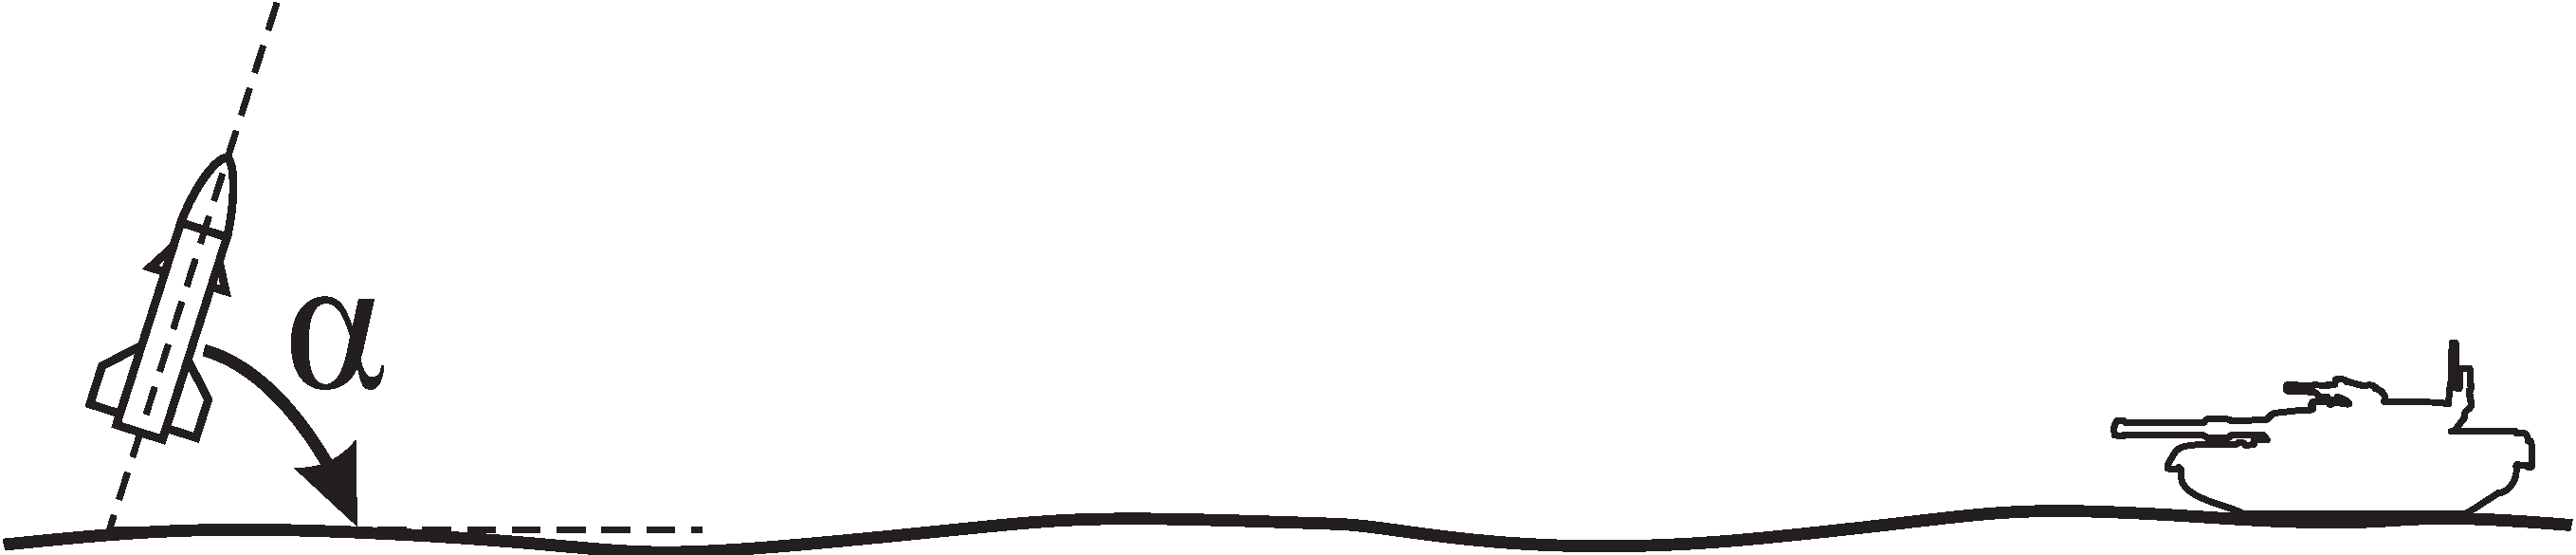
\includegraphics[width=0.475\textwidth]{rys05/alfa1} & 
%   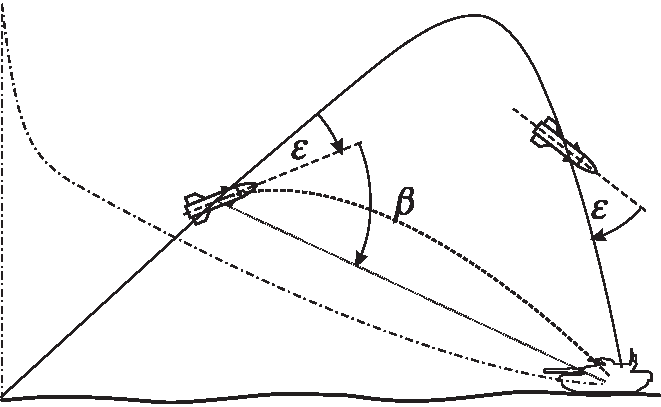
\includegraphics[width=0.475\textwidth]{rys05/beta1}
% 	% jeśli obraki są różnej wysokości, można je wyrównać do góry stosując vtop jak niżej
% 	% \vtop{\vskip-2ex\hbox{{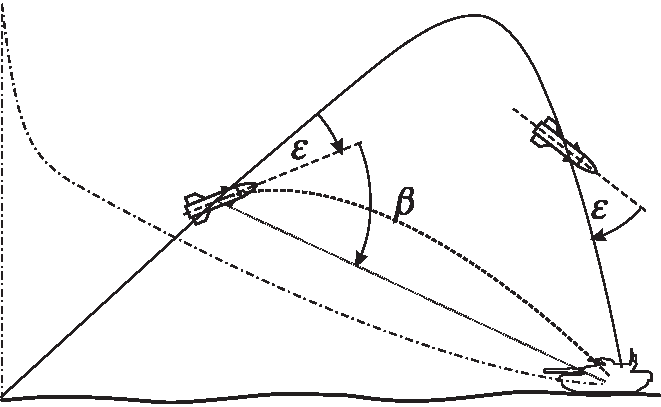
\includegraphics[width=0.475\textwidth]{rys05/beta1}}}} &
% 	% \vtop{\vskip-2ex\hbox{{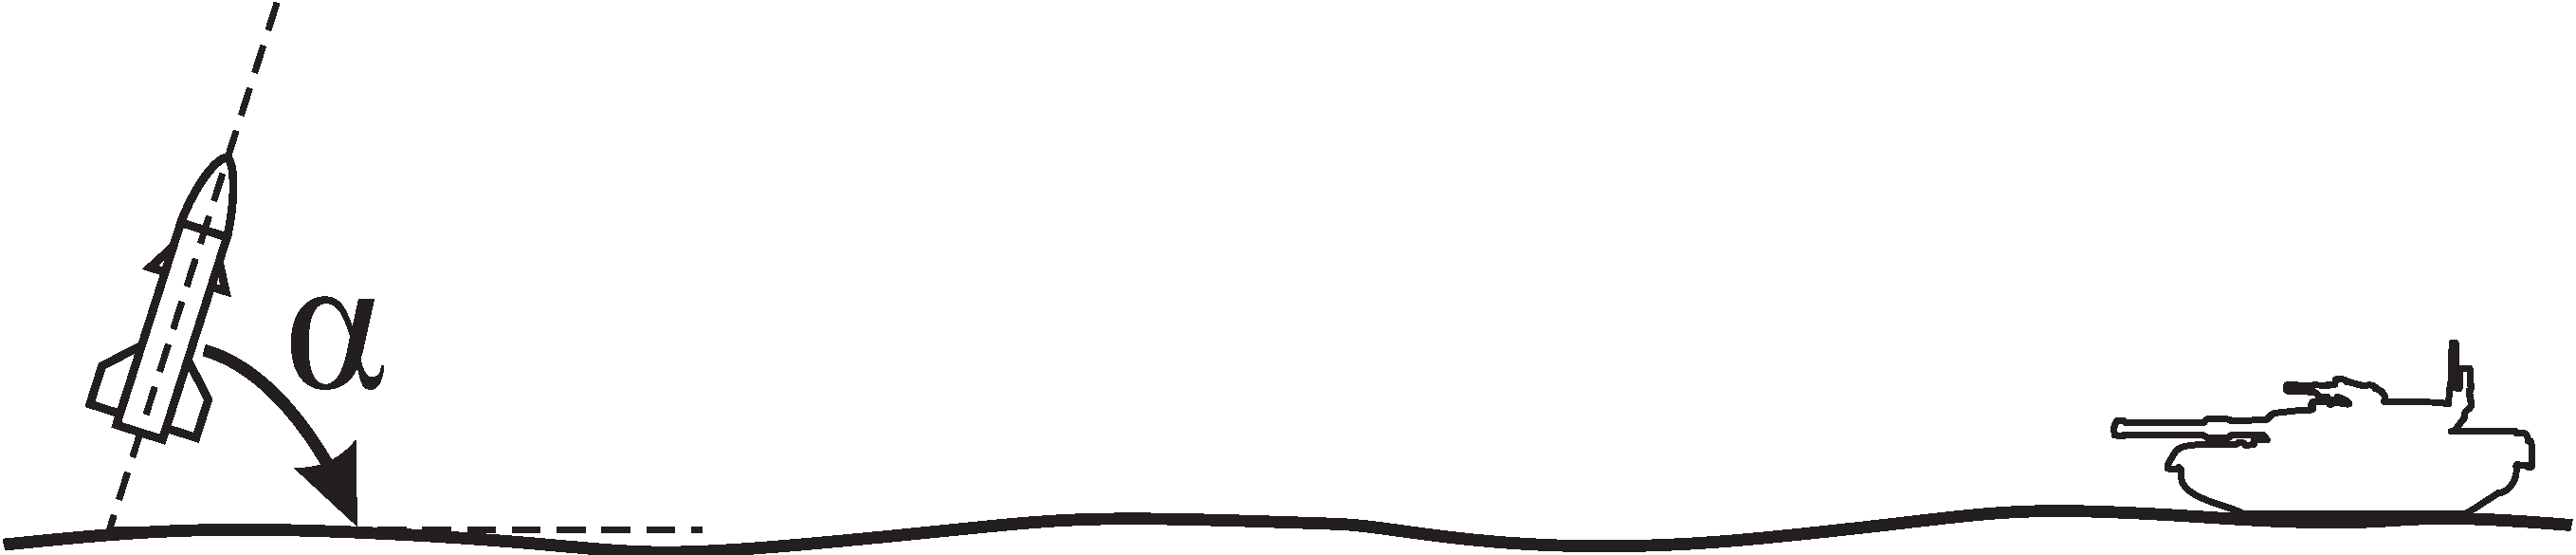
\includegraphics[width=0.475\textwidth]{rys05/alfa1}}}} 
%   \end{tabular}
%  a) trzy podejścia, b) podejście praktyczne}
%  \label{fig:alfabeta}
% \end{figure}
% \end{lstlisting}

% \begin{figure}[ht]
% 	\centering
% 		
\includegraphics[width=0.3\linewidth]{rys05/kanji-giri}
% 	\caption{Dwa znaki kanji -- giri}
% 	\label{fig:kanji-giri}
% \end{figure}

% \begin{figure}[htb]
%   \centering
% 	\begin{tabular}{@{}ll@{}}
% 	a) & b) \\
%   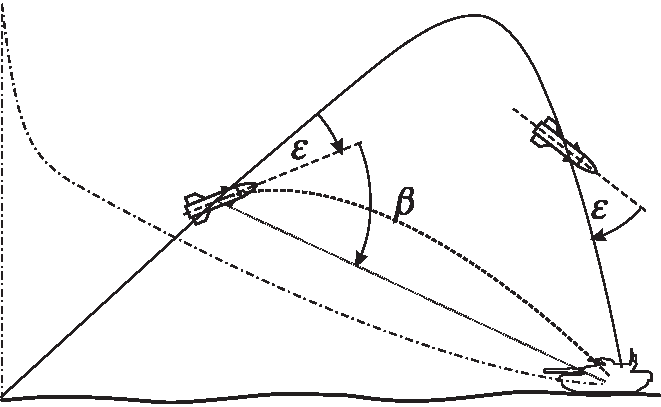
\includegraphics[width=0.475\textwidth]{rys05/beta1} & 
% 	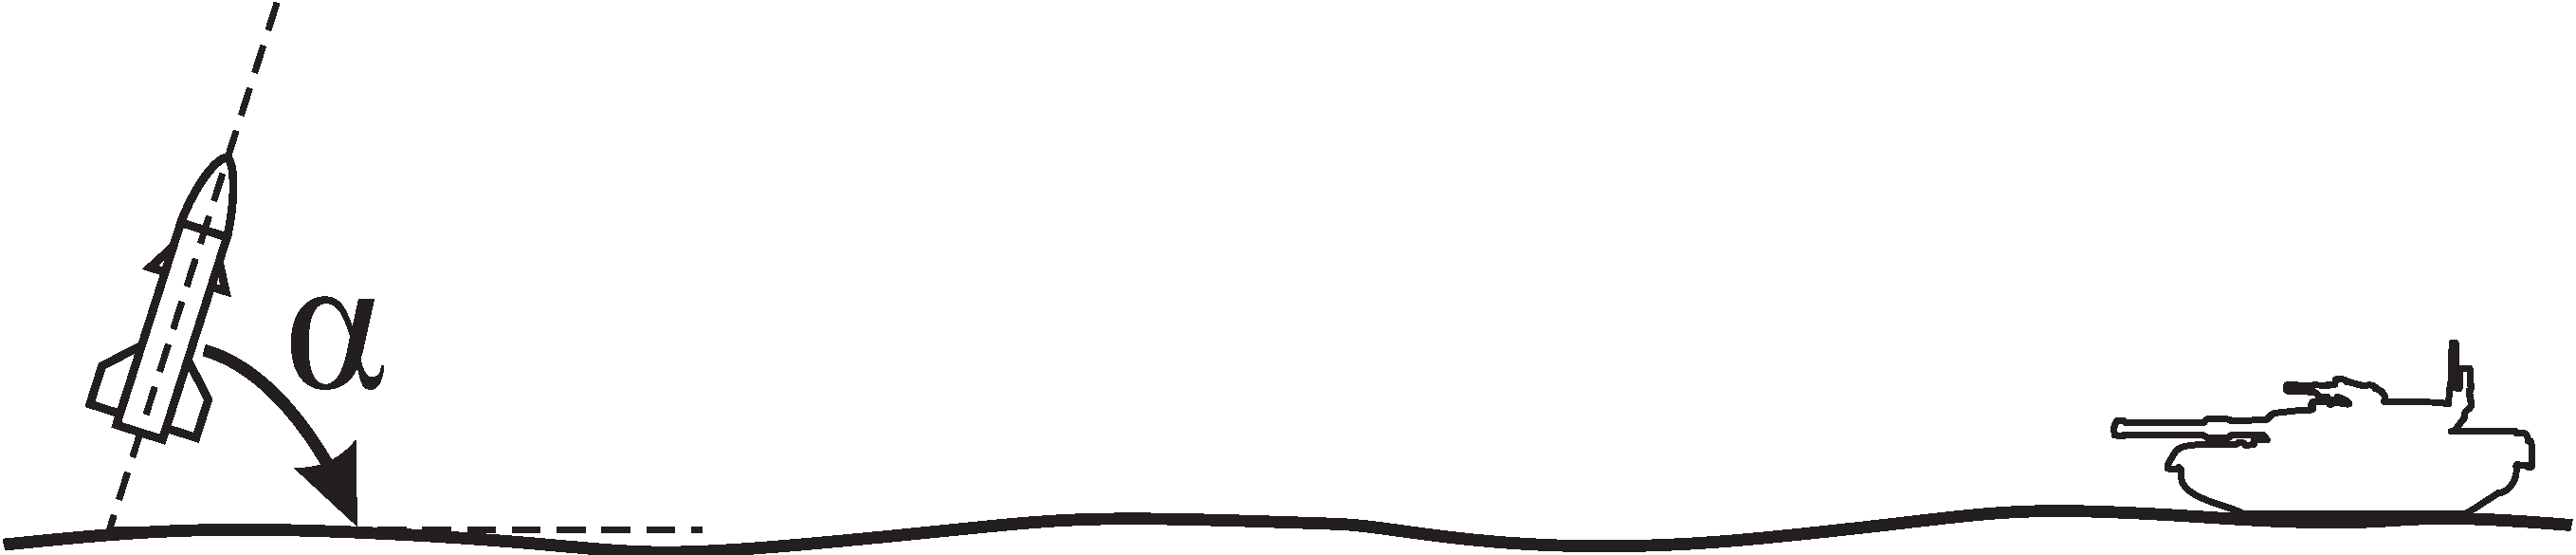
\includegraphics[width=0.475\textwidth]{rys05/alfa1}
% 	% jeśli obraki są różnej wysokości, można je wyrównać do góry stosując vtop jak niżej
% 	% \vtop{\vskip-2ex\hbox{{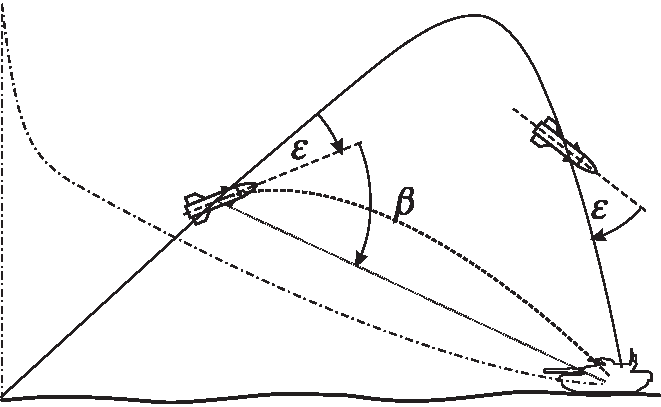
\includegraphics[width=0.475\textwidth]{rys05/beta1}}}} &
% 	% \vtop{\vskip-2ex\hbox{{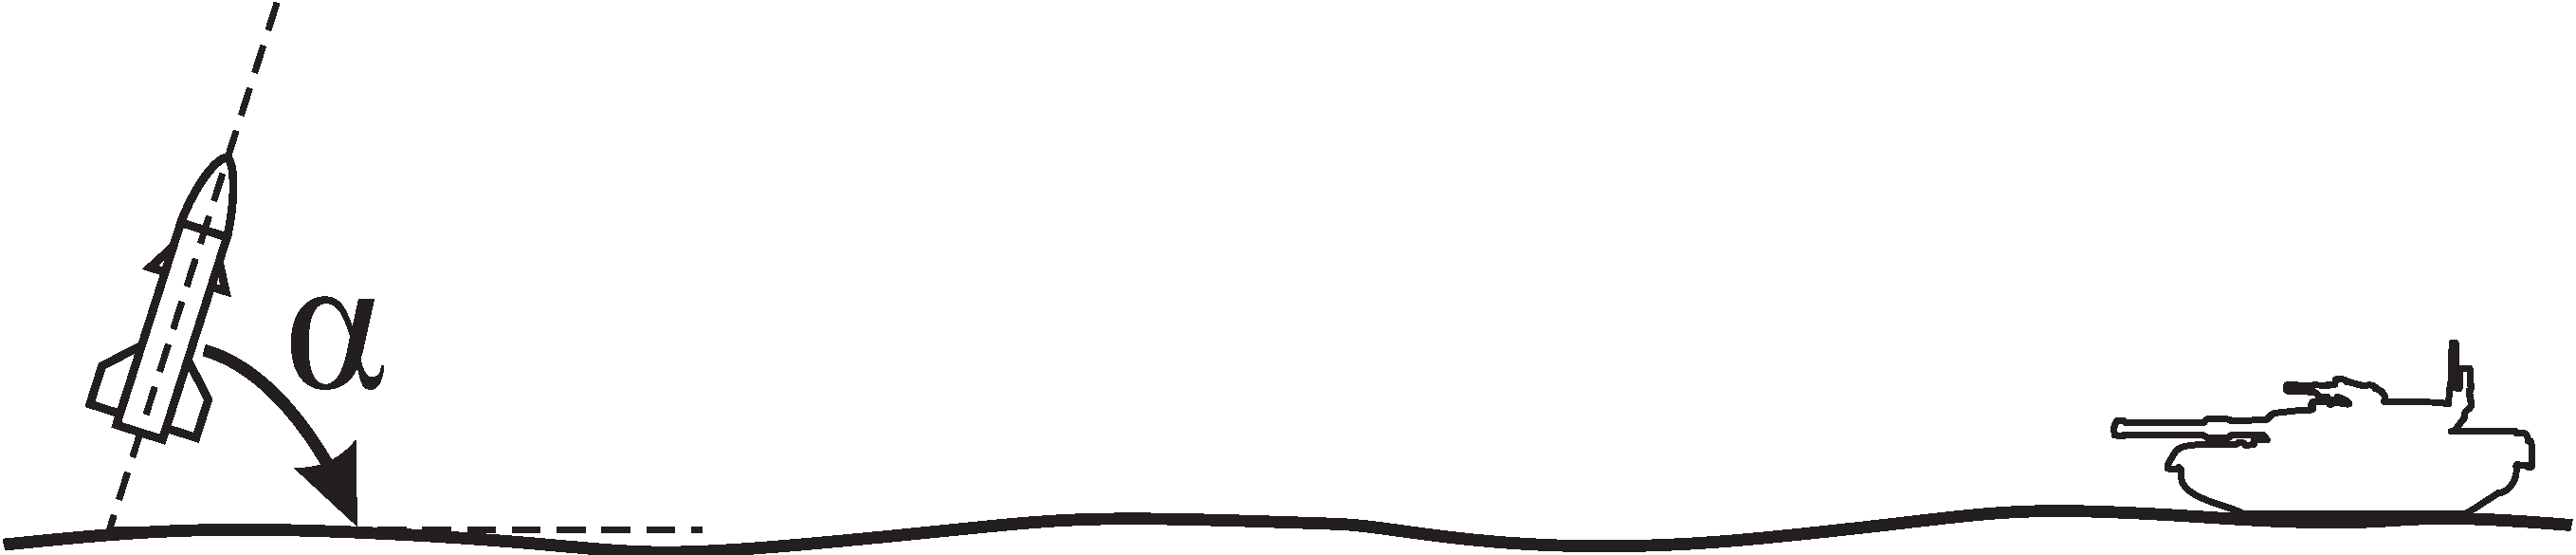
\includegraphics[width=0.475\textwidth]{rys05/alfa1}}}}  \caption{Wyznaczanie trajektorii lotu rakiety: 
% 	\end{tabular}
%   \caption{Wyznaczanie trajektorii lotu rakiety: a) trzy podejścia, b) podejście praktyczne}
%   \label{fig:alfabeta}
% \end{figure}

% Grafiki wektorowe powinny być dostarczone w plikach pdf. Rozmiar strony w~pliku pdf powinien być równy lub minimalnie większy od rozmiaru znajdującej się na nim grafiki (proszę spojrzeć na przykłady grafik wykorzystanych w niniejszym szablonie). Chodzi o to, aby na rysunku nie pojawiała się niepotrzebna biała przestrzeń (rozmiar płótna ma odpowiadać rozmiarowi grafiki bez żadnych marginesów, elementy grafiki powinny być ciasno ułożone). Grafiki rastrowe (głównie zrzuty z ekranu bądź zdjęcia) powinny być dostarczane w plikach o formacie \texttt{png} z~kompresją bezstratną. Zastosowanie kompresji stratnej, jak \texttt{jpg}, wprowadza niepotrzebne artefakty. Podobnie jak w przypadku grafik wektorowych, grafiki rastrowe nie powinny mieć białych marginesów.

% Niezłym sposobem generowanie ładnej grafiki wektorowej, w szczególności diagramów, jest posłużenie się, kolejno, następującymi darmowymi narzędziami:
% \begin{itemize}
% \item w \texttt{diagrams.net} (dawniej \texttt{draw.io}): narysowanie diagramu i wyeksportowanie do pdf (bezpośrednio lub pośrednio, poprzez zapisanie pliku w formacie \texttt{svg}, a potem jego wyświetlenie w~przeglądarce internetowej i wydrukowanie do \texttt{pdf}),
% \item w \texttt{inkscape}: zaimportowanie \texttt{pdf}, rozdzielenie grupy, wykasowanie niepotrzebnych elementów (tła), zaznaczenie wszystkiego, przycięcie strony do zaznaczonych (Ctr-Shift-R), zapisanie jako \texttt{pdf}. 
% \end{itemize}

% Na rysunku~\ref{fig:diagramy} pokazano przykład dobrze i źle (od strony technicznej) narysowanego diagramu. Celowo pokazano ramki, by było widać marginesy. Normalnie ramek tych nie należy stosować.
% \begin{figure}[htb]
%   \centering
% 	\begin{tabular}{@{}ll@{}}
% 	a) & b) \\
%   \vtop{\vskip-2ex\hbox{\fbox{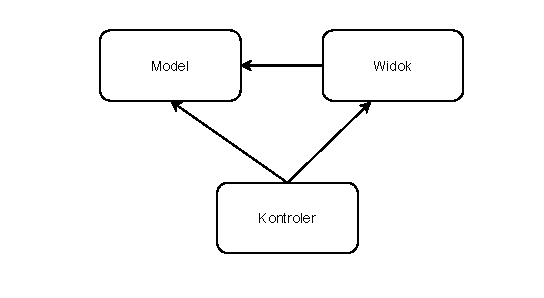
\includegraphics[width=0.4\linewidth]{rys05/diagram1}}}} & 
% 	\vtop{\vskip-2ex\hbox{\fbox{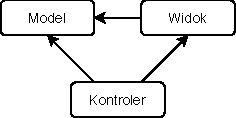
\includegraphics[width=0.4\linewidth]{rys05/diagram2}}}}
% 	% jeśli obraki są różnej wysokości, można je wyrównać do góry stosując vtop jak niżej
% 	% \vtop{\vskip-2ex\hbox{{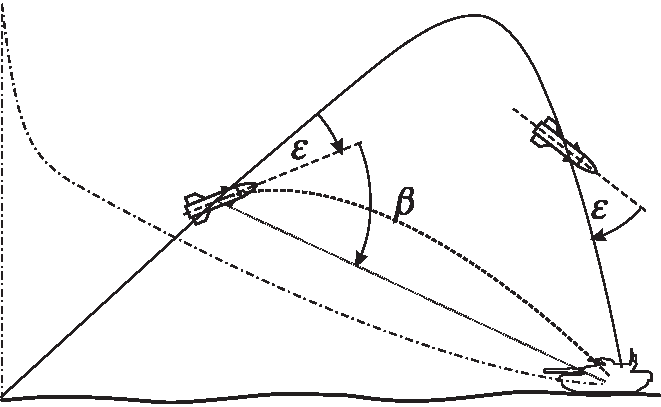
\includegraphics[width=0.475\textwidth]{rys05/beta1}}}} &
% 	% \vtop{\vskip-2ex\hbox{{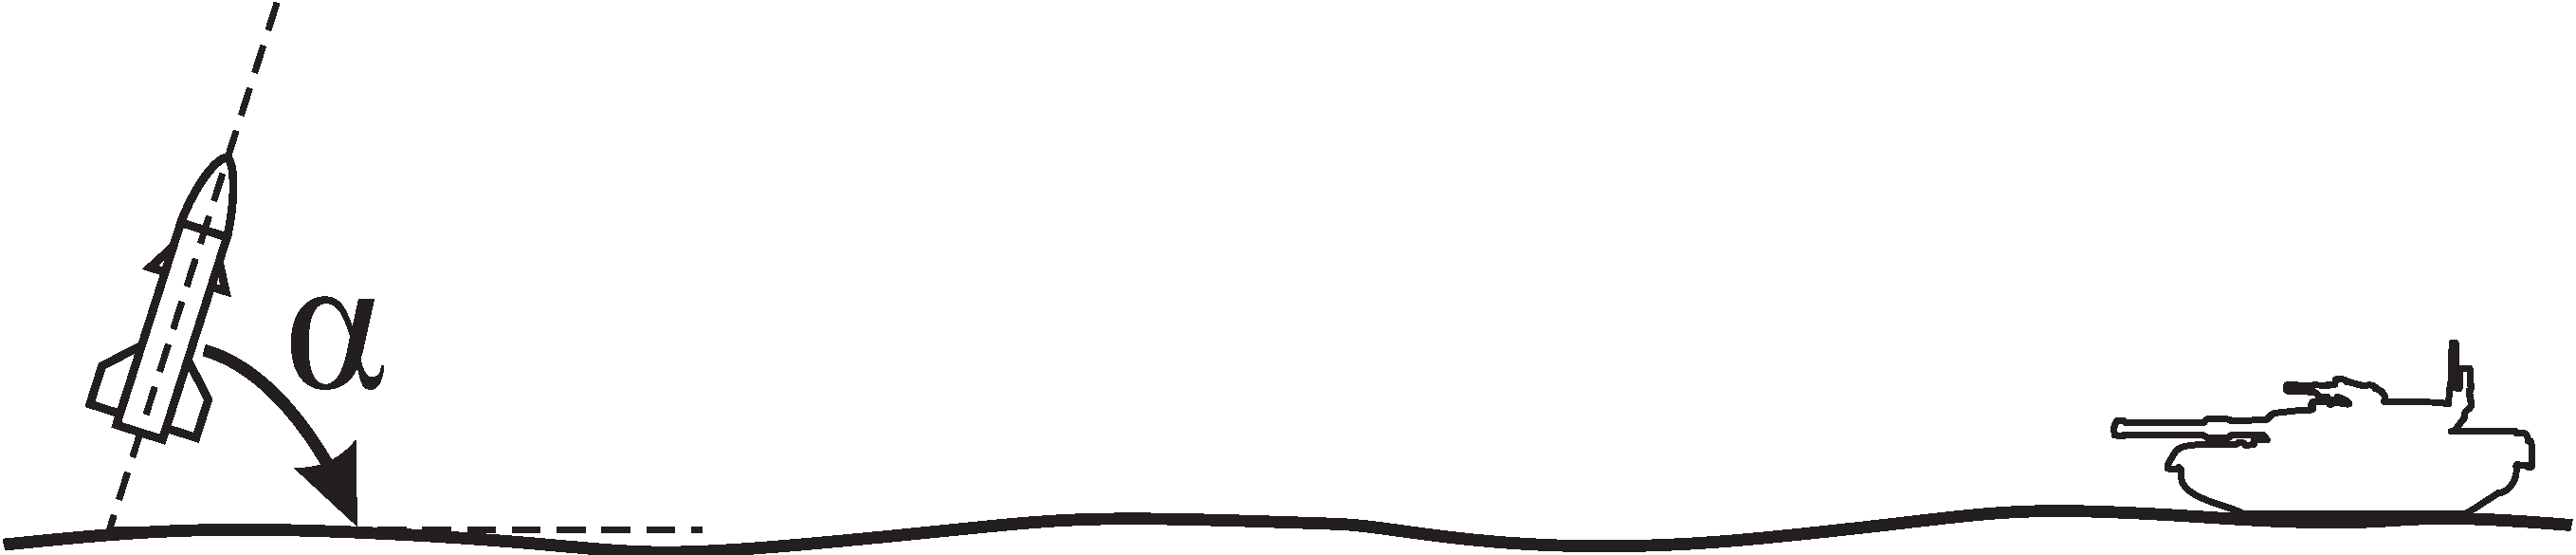
\includegraphics[width=0.475\textwidth]{rys05/alfa1}}}}  \caption{Wyznaczanie trajektorii lotu rakiety: 
% 	\end{tabular}
%   \caption{Przykład diagramu: a) złego, b) w miarę dobrego}
%   \label{fig:diagramy}
% \end{figure}

% Elementy na rysunkach nie powinny być wypełnione 100\% czernią ponieważ na wydrukach tworzą się plamy przebijające się przez kartkę. Zamiast tego wypełnienie elementów powinno być ustawione na ok.\ 90\% czerni.

% Czcionka na rysunkach nie może być większa od czcionki wiodącej tekstu (jedyny wyjątek to np.\ jakieś nagłówki).
% Należy stosować czcionkę kroju Arial, Helvetica bądź tego samego kroju co czcionka dokumentu (\texttt{texgyre-termes}). 

% Jeśli na jednym rysunku pojawić się ma kilka grafik, to zamiast stosować \texttt{subfigure} lub inne otoczenia należy: dostarczyć tabelę z wstawionymi do niej rysunkami, opcjonalnie adnotować jej części (np.~a) i b)), odnieść się do tych części w podpisie (posługując się adnotacjami, jak to zrobiono na rysunkach~\ref{fig:alfabeta} i \ref{fig:diagramy}, lub opisem słownym, np.~,,z lewej strony pokazano ...'', ,,po prawej zamieszczono ...'').

% Jeśli na rysunku zamieszczono w tabeli kilka grafik, to ich pozycjonowaniem (wyjustowaniem od góry) można manipulować za pomocą komendy:
% \verb+\vtop{\vskip-2ex\hbox{\includegraphics[width=0.475\textwidth]{nazwa}}}+

% Na rysunkach nie wolno nadużywać kolorów oraz ozdobników (wiele narzędzi do tworzenia diagramów dostarcza grafikę z cieniowaniem, gradacją kolorów itp.\  co niekoniecznie przekłada się na czytelność rysunku).
% Jeśli rysunki są kolorowe, to kolory te powinny być rozróżnialne po konwersji do poziomów szarości (chodzi o to, aby na wydrukach wykonanych na drukarkach monochromatycznych można było dostrzec różnice).

% Podczas robienia zrzutów z ekranu należy zadbać o to, by taki zrzut był czytelny po wydrukowaniu. Czyli aby pojawiające się literki były wystarczająco duże, a przestrzenie bez treści -- relatywnie małe. Przystępując do robienia zrzutu trzeba odpowiednio wyskalować elementy na ekranie. Na przykład robiąc zrzut z przeglądarki FF najpierw należy wcisnąć CTR--0 (domyślne skalowanie), potem CTR--{}- (zmniejszenie skali o stopień). Potem dobrze jest zawęzić okno przeglądarki tak, by interesująca treść wypełniła je w całości. Jeśli na obserwowanej stronie jest zbyt dużo pustych obszarów, to należy je jakoś zawęzić (sterując wielkością okna przeglądarki lub aktywnymi elementami interfejsu użytkownika). Zrzut bowiem wcale nie musi być odzwierciedleniem 1:1 domyślnego układu obserwowanych elementów. Ważne jest, by na zrzucie pokazać interesujący, opisywany fragment i żeby ten fragment był czytelny. Nie trzeba też zawsze robić zrzutów w układzie 16:9 (lub innym panoramicznym). Czasem lepiej jest zrobić zrzuty okien niemal kwadratowych, bo lepiej się układają w wynikowym dokumencie. Poza tym można je przeskalować (powiększyć) by zajmowały całą szerokość strony, a wtedy czcionka na wydrukach będzie większa. Takie skalowanie dla zrzutów panoramicznych zwykle się nie udaje. Na rysunku~\ref{fig:zrzuty} pokazano przykłady dobrze i źle zrobionych zrzutów (w celu oszczędzenia miejsca zrzuty umieszczono obok siebie).

% \begin{figure}[htb]
%   \centering
% 	\begin{tabular}{@{}ll@{}}
% 	a) & b) \\
%   \vtop{\vskip-2ex\hbox{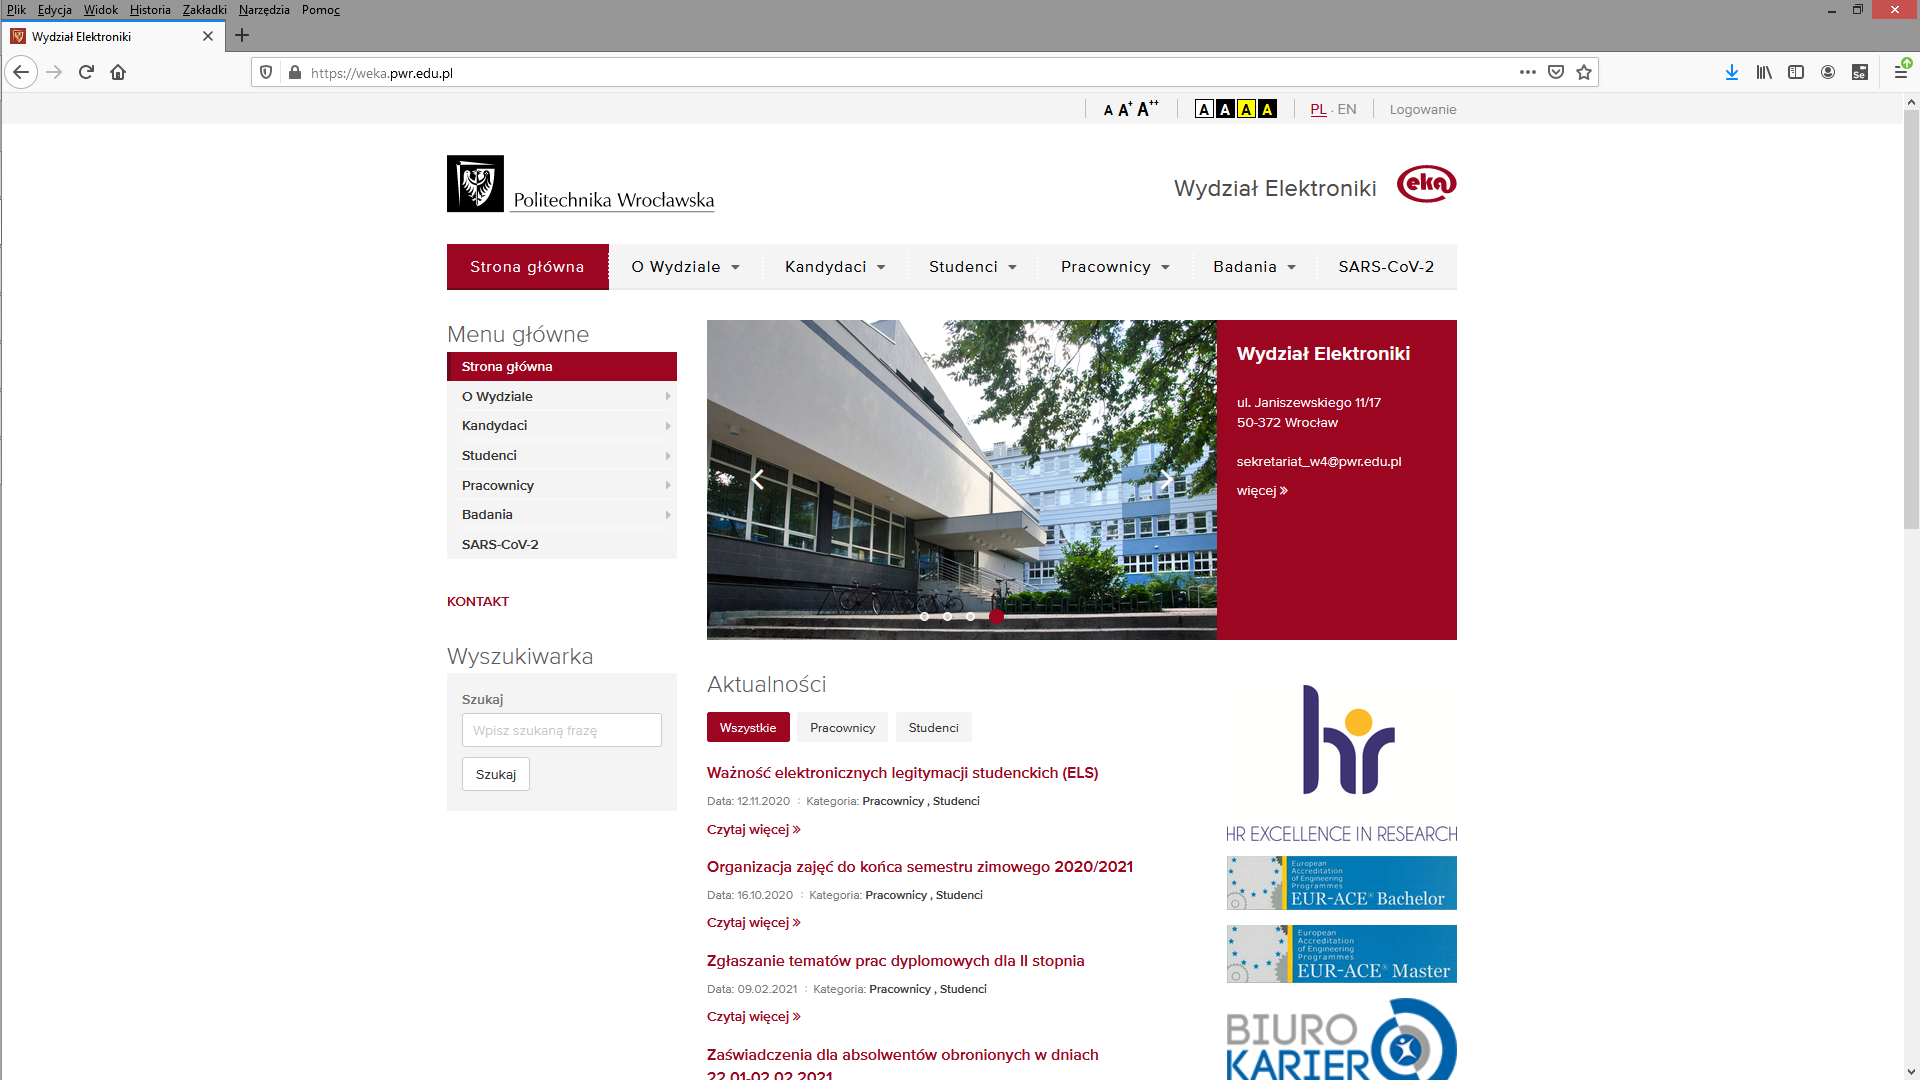
\includegraphics[width=0.475\textwidth]{rys05/zrzut1}}} & 
% 	\vtop{\vskip-2ex\hbox{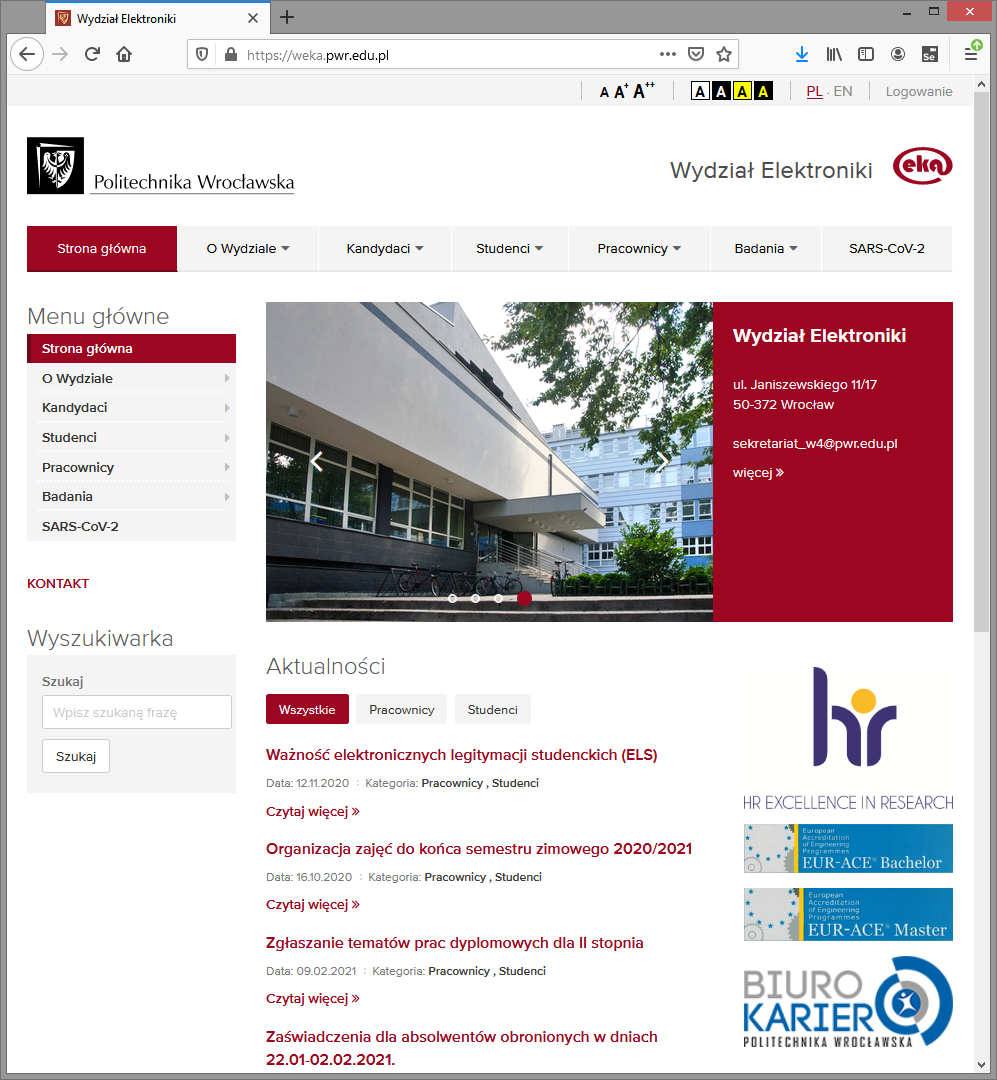
\includegraphics[width=0.475\textwidth]{rys05/zrzut2}}}
% 	% jeśli obraki są różnej wysokości, można je wyrównać do góry stosując vtop jak niżej
% 	% \vtop{\vskip-2ex\hbox{{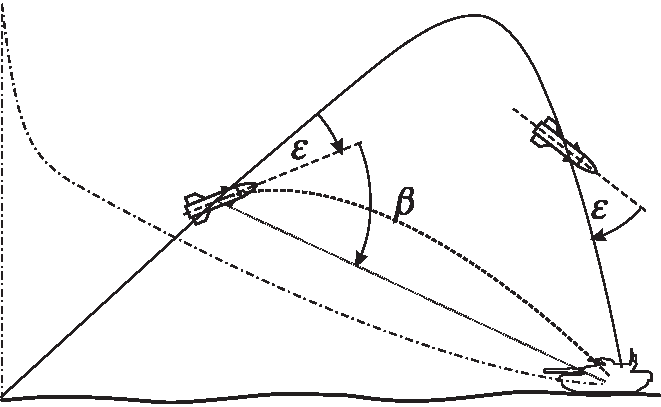
\includegraphics[width=0.475\textwidth]{rys05/beta1}}}} &
% 	% \vtop{\vskip-2ex\hbox{{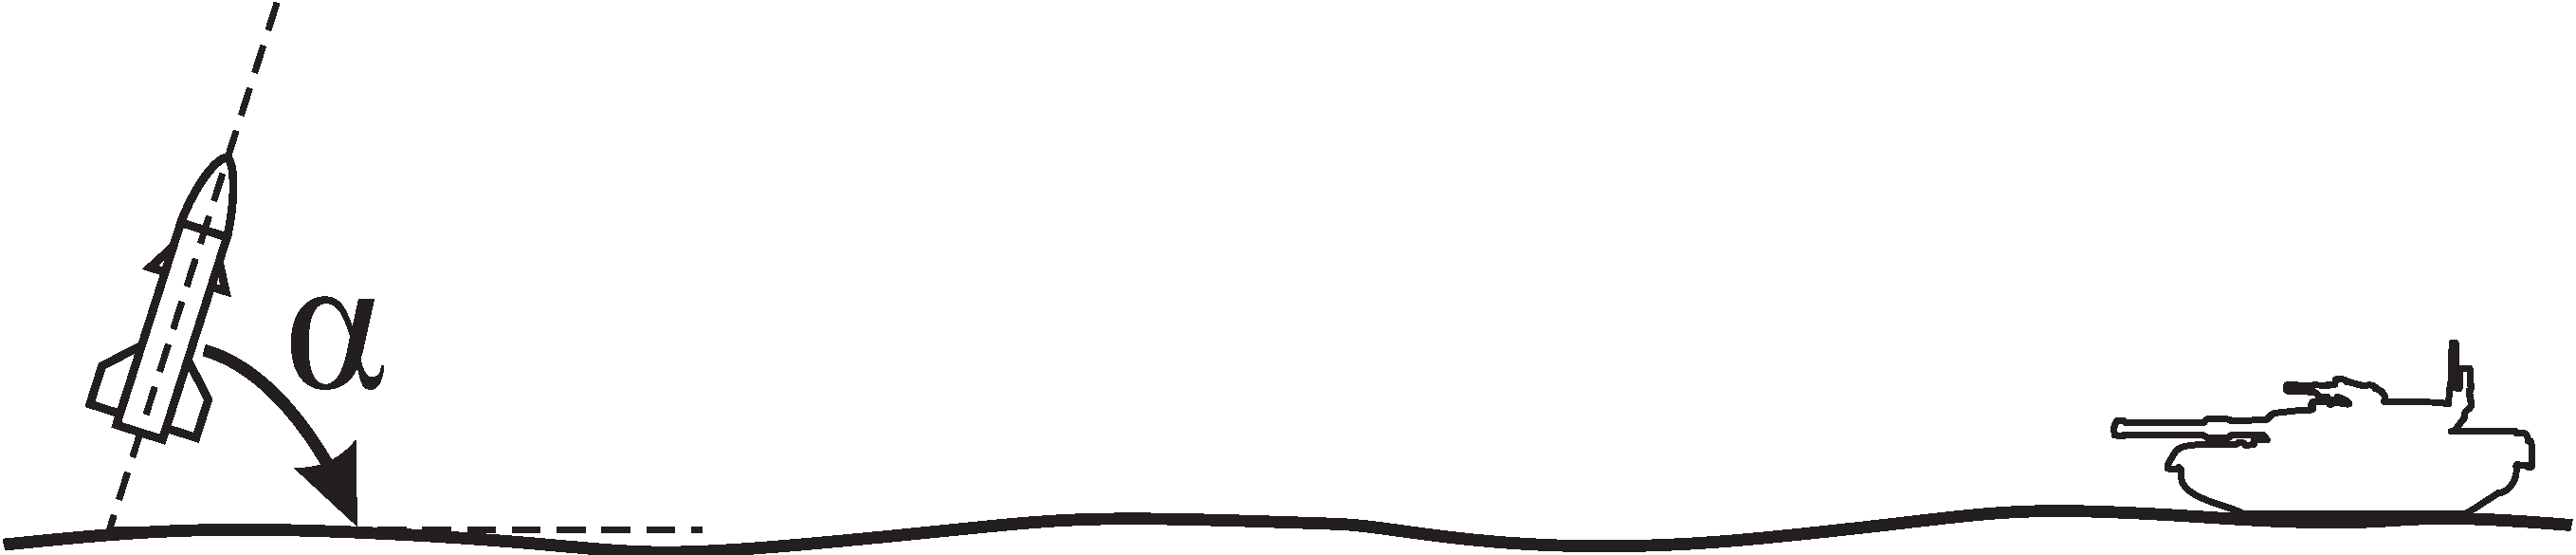
\includegraphics[width=0.475\textwidth]{rys05/alfa1}}}}  \caption{Wyznaczanie trajektorii lotu rakiety: 
% 	\end{tabular}
%   \caption{Przykłady zrzutów z ekranu: a) zły (nieczytelny, zrobiony przy zbyt szerokim oknie, z niepotrzebnymi marginesami, niepotrzebnym paskiem menu), b) w miarę dobry (w miarę czytelny, zrobiony przy zawężonym oknie, byłoby wskazane jeszcze usunięcie z niego beleczki z faviconem (jeśli nic nie wnosi) oraz przycięcie od dołu (jeśli treści tam pokazywane nie są istotne))}
%   \label{fig:zrzuty}
% \end{figure}


% Czasem problemem jest tworzenie zrzutów z ekranu, gdy występują na nim dane wrażliwe. Istnieją dwa sposoby na radzenie sobie z tym problemem.
% Pierwszy polega na zastąpieniu w~systemie danych danych rzeczywistych danymi testowymi -- wygenerowanymi tylko do celów prezentacji.
% Zrzut robi się wtedy na bazie danych testowych.
% Drugi polega na wykonaniu zrzutu z~ekranu, na którym pokazano dane rzeczywiste, i następnie zamianie tych danych już w pliku graficznym
% za pomocą odpowiedniego edytora (np.~\texttt{gimp}). Czyli oryginalny zrzut z ekranu należy otworzyć w edytorze, a potem
% nadpisać oryginalny tekst własnym tekstem. Konieczne jest wtedy dobranie odpowiednich czcionek aby nie było widać
% wprowadzonych zmian. 
% \begin{quotation}
% Uwaga: takie manipulowanie zrzutami jest usprawiedliwione jedynie w przypadku konieczności ochrony danych wrażliwych czy też lepszego pokazania wybranych elementów. Nie może to prowadzić generowania fałszywych rezultatów!!!
% \end{quotation}

% \section{Wstawianie kodu źródłowego}
% Kod źródłowy można wstawiać jako blok tekstu pisany czcionką maszynową. Używa się do tego otoczenie \verb?\lstlisting?. W atrybutach otoczenia można zdefiniować tekst podpisu wstawianego wraz z numerem nad blokiem, etykietę do tworzenia odwołań, sposób formatowania i~inne ustawienia. Zaleca się stosowanie w tym otoczeniu następujących parametrów:
% \begin{lstlisting}[basicstyle=\footnotesize\ttfamily]
% \begin{lstlisting}[label=list:req1,caption=Initial HTTP Request,
%                    basicstyle=\footnotesize\ttfamily]
% \end{lstlisting}
% Szczególnie przydatne podczas wstawiania większej ilości kodu źródłowego jest zastosowanie parametru \verb+basicstyle=\footnotesize\ttfamily+. Dzięki niemu zmniejsza się czcionka, a~przez to na stronie można zmieścić dłuższe linijki kodu. Użycie tak zdefiniowanego parametru nie jest jednak sztywnym zaleceniem. Wielkość czcionki można dobierać do potrzeb. 
% {\belowcaptionskip=-10pt
% \begin{lstlisting}[label=list:req1,caption=Initial HTTP Request,
%                    basicstyle=\footnotesize\ttfamily]
% GET /script/Articles/Latest.aspx HTTP/1.1
% Host: www.codeproject.com
% Connection: keep-alive
% Cache-Control: max-age=0
% Accept: text/html,application/xhtml+xml,application/xml
% User-Agent: Mozilla/5.0 ...
% Accept-Encoding: gzip,deflate,sdch
% Accept-Language: en-US...
% Accept-Charset: windows-1251,utf-8...
% \end{lstlisting}
% }
% Można też sformatować kod bez stosowania numerowanego podpisu (wtedy nie zamieszcza się \texttt{caption} na liście atrybutów).
% \begin{lstlisting}[basicstyle=\footnotesize\ttfamily]
% GET /script/Articles/Latest.aspx HTTP/1.1
% Host: www.codeproject.com
% Connection: keep-alive
% Cache-Control: max-age=0
% Accept: text/html,application/xhtml+xml,application/xml
% User-Agent: Mozilla/5.0 ...
% Accept-Encoding: gzip,deflate,sdch
% Accept-Language: en-US...
% Accept-Charset: windows-1251,utf-8...
% \end{lstlisting}

% Ponadto istnieje kilka sposobów wstawiania kodu źródłowego w bieżącej linijce tekstu:
% \begin{itemize} 
% \item korzystając z polecenia \verb?\texttt? ustawiającego czcionkę maszynową, jak w przykładzie \texttt{tutaj} (efekt zastosowania komendy \verb?\texttt{tutaj}?). Problemem jednak mogą okazać się znaki podkreślenia i inne znaki kontrolne.
% \item korzystają z otoczenia \verb?\verb? zapewniającego wypisanie kodu czcionką maszynową jak w~przykładzie \verb|tutaj| (efekt zastosowania komendy \verb?\verb|tutaj|?). Problemem jest to, że polecenie \verb?\verb? nie potrafi łamać dłuższego tekstu.
% \item korzystając z polecenia \verb?\lstin? umożliwiającego wypisanie kodu czcionką ustawianą w~opcjach jak w przykładzie
% \lstset{basicstyle=\ttfamily}\lstinline{tutaj} (efekt komendy \verb+\lstset{basicstyle=\ttfamily}\lstinline{tutaj}+) lub \lstinline[basicstyle=\ttfamily]=tutaj= (efekt komendy \verb+\lstinline[basicstyle=\ttfamily]=tutaj=+).
% \end{itemize}

% Poniżej zamieszczono przykłady kodów źródłowych z podświetleniem składni.

% \begin{lstlisting}[language=Java,style=JavaStyle,caption=Opis 1, label=lst:pierwszy]
% package pl.mrbarozoit.backend;

% import org.springframework.boot.SpringApplication;
% import org.springframework.boot.autoconfigure.SpringBootApplication;

% @SpringBootApplication
% public class BackendApplication {

%     public static void main(String[] args) {
%         SpringApplication.run(BackendApplication.class, args);
%     }

% }
% \end{lstlisting}

% Jeśli w kodzie źródłowym jest jakiś nieistotny fragment względem omawianego problemu, to można go wykropkować (patrz listing~\ref{lst:drugi}).

% {\belowcaptionskip=-9pt % To polecenie zmniejszy odległość podpisu od pokazywanego kodu (jego stosowanie jest zalecane)
% \begin{lstlisting}[language=JavaScript,style=JavaScriptStyle,caption=Opis 2, label=lst:drugi]
% // Karma configuration file, see link for more information
% // https://karma-runner.github.io/1.0/config/configuration-file.html

% module.exports = function (config) {
%   config.set({
%     basePath: '',
%     frameworks: ['jasmine', '@angular-devkit/build-angular'],
%     plugins: [
%       require('karma-jasmine'),
%       require('karma-chrome-launcher'),
%       require('karma-jasmine-html-reporter'),
%       require('karma-coverage-istanbul-reporter'),
%       require('@angular-devkit/build-angular/plugins/karma')
%     ],
%     ... // opuszczony kod
%     autoWatch: true,
%     browsers: ['Chrome'],
%     singleRun: false,
%     restartOnFileChange: true
%   });
% };
% \end{lstlisting}
% }

% Jeśli kod jest wąski, to można sformatować go w dwóch kolumnach jak na listingu~\ref{lst:kontrakt-board-move-in}.

% % Trzeba zacząć po linijce przerwy
% \begingroup 
% \listingcaption{Kontrakt na model wejściowy endpointu \texttt{/api/v1/chess/board/move}}
% \setlength\multicolsep{0pt plus 2pt}%
% \begin{lstlisting}[style=json-style, multicols=2, label=lst:kontrakt-board-move-in]
% {
%    "lastPosition": {
%       "fenDescription": "string"
%    },
%    "image": {
%       ...
%    },
%    "positions": {
%       "chessboardCorners": [
%          ...
%       ],
%       "tilesCornerPoints": [
%          ...
%       ]
%    },
%    "referenceColors": {
%       ...
%    },
% }
% \end{lstlisting}
% \vspace{6pt plus 2pt}
% \endgroup

% \section{Wykaz literatury oraz cytowania}
% \label{sec:literatura}
% Cytowania powinny być zamieszczane w tekście z użyciem komendy \verb+\cite{}+. Jej argumentem powinien być klucz cytowanej pozycji (lub lista kluczy  rozdzielonych przecinkiem bez spacji, jeśli takich pozycji w danym miejscu cytuje się więcej) jaki jest używany w bazie danych bibliograficznych (plik \texttt{dokumentacja.bib}). Po kompilacji \texttt{bibtex} i \texttt{pdflatex} w tekście pojawia się właściwy odsyłacz do pozycji w wykazie literatury (ujęty w kwadratowe nawiasy -- zgodnie z~tym, co definiuje styl \texttt{plabbrv.bst}), zaś w samym wykazie (rozdział Literatura) -- zacytowana pozycja. Przykładem cytowania jest: ,,dobrze to opisano w pracach~\cite{JS07,SQL2}'' (gdzie zastosowano komendę \verb?\cite{JS07,SQL2}?).

% Co do zawartości rekordów bibliograficznych - style bibtexowe potrafią ,,skracać'' imiona (czyli wstawiać, jeśli taka wola, inicjały zamiast pełnych imion). Niemniej dobrze jest od razu przyjąć jakąś konwencję. Proponuje się, aby w rekordach od razu wstawiane były inicjały zamiast pełnych imion.

% Niekiedy tytuły prac zawierają wyrazy z dużymi i małymi literami. Takie tytuły należy brać w podwójne nawiasy klamrowe, aby \texttt{bibtex} nie zamienił ich na postać, w której poza pierwszą literą pozostałe są małe.

% Jeśli jakiś cytowany zasób pochodzi z Internetu, to jego rekord w pliku \texttt{bib} powinien wyglądać jak niżej.
% \begin{lstlisting}[basicstyle=\footnotesize\ttfamily]
% @INPROCEEDINGS{SQL2, 
%   title={{A MySQL-based data archiver: preliminary results}}, 
%   author={Bickley, M. and Slominski, Ch.},
%   booktitle = {{Proceedings of ICALEPCS07}},
% 	month = oct,
% 	day = {15--19},
% 	year={2007}, 
%   note={\url{http://www.osti.gov/scitech/servlets/purl/922267} 
% 	[dostęp dnia 20 czerwca 2015]}
% }
% \end{lstlisting}
% A to inny przykład rekordu danych bibliograficznych:
% \begin{lstlisting}[basicstyle=\footnotesize\ttfamily]
% @TechReport{JS07,
% 	author = {Jędrzejczyk, J. and Śródka, B.},
% 	title  ={Segmentacja obrazów metodą drzew decyzyjnych},
% 	year = {2007},
% 	institution = {Politechnika Wrocławska, Wydział Elektroniki}
% }
% \end{lstlisting}

% \section{Indeks rzeczowy}
% \label{sec:indeks}
% Generowanie indeksu \index{generowanie!-- indeksu} po trosze wygląda jak generowanie wykazu literatury \index{generowanie!-- wykazu literatury}-- wymaga kilku kroków. Podczas pierwszej kompilacji \texttt{pdflatex} generowany jest plik z rozszerzeniem \texttt{*.idx} (zawierający ,,surowy indeks''). Następnie, bazując na tym pliku, generowany jest plik z rozszerzeniem \texttt{*.ind} zawierający sformatowane dane. Ten krok wymaga uruchomienia odpowiedniego narzędzia oraz zastosowania plik z definicją stylu \texttt{Dyplom.ist}. W kroku ostatnim dokonuje się kolejnej kompilacji \texttt{pdflatex} (dzięki niej w wynikowym dokumencie pojawi się Indeks rzeczowy). Domyślnie Indeks rzeczowy zostanie sformatowany w~układzie dwukolumnowym.

% Oczywiście aby to wszystko zadziałało w kodzie szablonu należy umieścić odpowiednie komendy definiujące elementy indeksu rzeczowego (\verb?\index?) oraz wstawiające sformatowany Indeks rzeczowy do dokumentu wynikowego (\verb?\printindex?). Więcej informacji o tworzeniu indeksu rzeczowego można znaleźć na stronie \url{https://en.wikibooks.org/wiki/LaTeX/Indexing}. Poniżej przedstawiono przykłady komend użytych w szablonie do zdefiniowania elementów indeksu rzeczowego:
% \begin{itemize}
% \item \verb?\index{linia komend}? -- pozycji główna.
% \item \verb?\index{generowanie!-- indeksu}? -- podpozycja.
% \end{itemize}

% Generowanie pliku \texttt{*.ind} można inicjować na kilka sposobów:
% \begin{itemize}
% \item poprzez wydanie odpowiedniego polecenia bezpośrednio w linii komend \index{linia komend}
% \begin{lstlisting}[basicstyle=\footnotesize\ttfamily]
% makeindex Dyplom.idx -t Dyplom.ilg -o Dyplom.ind -s Dyplom.ist
% \end{lstlisting}
% \item poprzez odpalenie odpowiedniego narzędzia środowiska. Na przykład w \texttt{TeXnicCenter} definiuje się tzw. \texttt{output profiles}: 
% \begin{lstlisting}[basicstyle=\footnotesize\ttfamily]
% makeindex "%tm.idx" -t "%tm.ilg" -o "%tm.ind" -s "%tm.ist"
% \end{lstlisting}
% a samo generowanie pliku \texttt{*.ind} zapewni wybranie pozycji menu \texttt{Build/Makeindex}.
% \item korzystając z odpowiednio sparametryzowanych pakietów i komend wewnątrz kompilowanego dokumentu (czyli od razu przy okazji jego kompilacji).
% \begin{lstlisting}[basicstyle=\footnotesize\ttfamily]
% \DisemulatePackage{imakeidx}
% \usepackage[noautomatic]{imakeidx} 
% % jeśli chcemy, by indeks by generowany automatycznie programem makeindex:
% %\usepackage[makeindex]{imakeidx} 
% % a tak ponoć można przekazać opcje do programu generującego indeks:
% %\makeindex[options=-s podrecznik -L polish -M lang/polish/utf8] 
% %\makeindex[options=-s podrecznik]
% \makeindex
% \end{lstlisting}

% Niestety, \texttt{makeindex} jest narzędziem, które umieszcza część pozycji w grupie \texttt{Symbols}, a~nie w grupach związanych z literkami alfabetu. W związku z czym indeksowany element zaczynający się od polskiej literki trafia do grupy \texttt{Symbols}, jak np.~\verb?\index{Światło}?\index{Światło}. Jeśli chce się zamieszczać w indeksie symbole matematyczne, to dobrze jest to robić jak w następującym przykładzie: \verb?\index{$asterisk@$\ast$}? \index{$asterisk@$\ast$} czy też \verb?\index{c@$\mathcal{C}$}?\index{c@$\mathcal{C}$}, tj.~dostarczając przy okazji klucz do sortowania.
% Lepiej w tym względzie radzą sobie inne narzędzia, jak \texttt{texindy} lub \texttt{xindy} dostępne pod linuxem. Korzystając z nich uzyskuje się grupy polskich literek w indeksie rzeczowym (hasła zaczynające się od polskich literek już nie trafiają do grupy Symbols). Przykład polecenia wydanego z linii komend, w którym wykorzystano \texttt{texindy} zamieszczono poniżej (zakładamy kodowanie plików w UTF8, można dla niniejszego szablonu zmienić na cp1250):
% \begin{lstlisting}[basicstyle=\footnotesize\ttfamily]
% texindy -L polish -M lang/polish/utf8 Dyplom.idx
% \end{lstlisting}

% To polecenie wygeneruje \texttt{Dyplom.ind} o zawartości:
% \begin{lstlisting}[basicstyle=\footnotesize\ttfamily]
% \begin{theindex}
%   \providecommand*\lettergroupDefault[1]{}
%   \providecommand*\lettergroup[1]{%
%       \par\textbf{#1}\par
%       \nopagebreak
%   }

%   \lettergroup{G}
%   \item generowanie
%     \subitem -- indeksu, 27
%     \subitem -- wykazu literatury, 27

%   \indexspace

%   \lettergroup{L}
%   \item linia komend, 27

%   \indexspace

%   \lettergroup{Ś}
%   \item \'Swiat\IeC {\l }o, 28

% \end{theindex}
% \end{lstlisting}


% \end{itemize}


% Aby mieć większą kontrolę automatyczne generowanie indeksu zostało w niniejszym szablonie wyłączone (indeks trzeba wygenerować samemu, wydając polecenie \texttt{makeindex} lub zalecane \texttt{texindy}).

% \section{Inne uwagi}
% Dobrym sposobem na kontrolę błędów występujących podczas kompilacji jest wstawianie linijki \verb?\end{document}? w wybranym miejscu dokumentu. Jest to szczególnie przydatne w przypadkach, gdy błędy te są trudne do zidentyfikowania (gdy wygenerowane przez kompilator numery linii z błędami nie są tymi, w których błędy występują). Wystarczy wtedy przestawić wspomnianą linijkę do kolejnych miejsc, aż znajduję to miejsce, gdzie występuje problem.

% Aby osiągnąć apostrofy maszynowe (złożone z samych kresek) należy użyć polecenia \verb?"{}jak tutaj{}"? (podwójny apostrof stojący bezpośrednio przed niektórymi literkami zamienia je na literki z akcentami, aby temu zapobiec dostawiono nawiasy klamrowe). W efekcie otrzymamy "{}jak tutaj{}". Jeśli natomiast apostrofy mają być drukarskie (złożone z kropek i kresek), to należy użyć polecenia \verb?,,jak tutaj''? (dwa pojedyncze przecinki i dwa pojedyncze apostrofy). W efekcie otrzymamy ,,jak tutaj''. Można też użyć znaków apostrofów odpowiednio zakodowanych „jak tutaj”, tylko że czasem trudno pisze się takie apostrofy w środowiskach kompilacji projektów latexowych.


% Oto sposoby ustawienia odstępów między liniami:
% \begin{itemize}
% \item używając komendy \verb+\linespread{...}+ (akceptowalne), przy czym atrybutem tej metody jest współczynnik zależny od wielkości
% czcionki.  Dla czcionki wiodącej 12pt odstęp półtora linii osiągnie się komendą \verb+\linespread{1.241}+. Dla innych czcionek wiodących wartości tego parametru są jak w poniższym zestawieniu.
% \begin{lstlisting}[basicstyle=\footnotesize\ttfamily]
% 10pt 1.25 dla \onehalfspacing 
%      1.667 for \doublespacing, 
% 		 ponieważ ,,basic ratio'' = 1.2 
% 		(\normalfont posiada \baselineskip rozmiaru 12pt)
% 11pt 1.213 dla \onehalfspacing oraz 1.618 dla \doublespacing, 
%      ponieważ ,,basic ratio'' = 1.236 
% 		(\normalfont posiada \baselineskip rozmiaru 13.6pt)
% 12pt 1.241 dla \onehalfspacing oraz 1.655 dla \doublespacing, 
%      ponieważsince ''basic ratio'' is 1.208 
% 		(\normalfont has a \baselineskip of 14.5pt)
% \end{lstlisting}
% Kłopot w tym, że raz ustawiony odstęp będzie obowiązywał do wszystkich czcionek (brak jest mechanizmu zmiany współczynnika w zależności od wielkości czcionki akapitu).

% \item używając pakietu \texttt{setspace} (niezalecane). Ponieważ klasa \texttt{memoir} emuluje pakiet \texttt{setspace}, w preambule dokumentu należałoby umieścić:
% \begin{lstlisting}[basicstyle=\footnotesize\ttfamily]
% \DisemulatePackage{setspace}
% \usepackage{setspace}
% \end{lstlisting}
% a potem można już sterować odstęp komendami:
% \begin{lstlisting}[basicstyle=\footnotesize\ttfamily]
% \singlespacing
% \onehalfspacing
% \doubelspacing
% \end{lstlisting}
% Ten sposób pozwala na korzystanie z mechanizmu automatycznej zmiany odległości linii w~zależności od wielkości czcionki danego akapitu.
% \item korzystając bezpośrednio z komend dostarczonych w klasie \texttt{memoir} (zalecane):
% \begin{lstlisting}[basicstyle=\footnotesize\ttfamily]
% \SingleSpacing
% \OnehalfSpacing
% \DoubleSpacing
% \end{lstlisting}
% Ten sposób również pozwala na korzystanie z mechanizmu automatycznej zmiany odległości linii w zależności od wielkości czcionki danego akapitu.
% \end{itemize}

% Na koniec jeszcze uwaga o rozmiarze pliku wynikowego. Otóż \texttt{pdflatex} generuje pliki \texttt{pdf}, które zazwyczaj mogłyby być nieco lepiej
% skompresowane. Do lepszego skompresowania tych plików można użyć programu \texttt{ghostscript}. Wystarczy w tym celu wydać komendę (pod windowsami):
% \begin{lstlisting}[basicstyle=\footnotesize\ttfamily]
% gswin64 -sDEVICE=pdfwrite -dCompatibilityLevel=1.4 -dNOPAUSE -dQUIET \
% -dSAFER -dBATCH -sOutputFile=Dyplom-compressed.pdf Dyplom.pdf
% \end{lstlisting}
% W poleceniu tym można również wstawić opcję \texttt{-dPDFSETTINGS=/prepress} (zapewniającą uzyskanie wysokiej jakości, zachowanie kolorów, uzyskanie obrazków w rozdzielczości 300 dpi). Ze względów licencyjnych ghostscript używa domyślnie algorytmów z kompresją stratną. Przy kompresji może więc dojść do utraty jakości bitmap.



\chapter{Podsumowanie}
\label{chap:podsumowanie}
% Podsumowanie jest miejscem, w którym należy zamieścić syntetyczny opis tego, o czym jest dokument. W szczególności w pracach dyplomowych w podsumowaniu powinno znaleźć się jawnie podane stwierdzenie dotyczące stopnia realizacji celu. Czyli powinny pojawić się w niej akapity ze zdaniami typu: ,,Podczas realizacji pracy udało się zrealizować wszystkie postawione cele''. Ponadto powinna pojawić się dyskusja na temat napotkanych przeszkód i sposobów ich pokonania, perspektyw dalszego rozwoju, możliwych zastosowań wyników pracy itp.

% \section{Sekcja poziomu 1}% 
% Lorem ipsum dolor sit amet eleifend et, congue arcu. Morbi tellus sit amet, massa. Vivamus est id risus. Sed sit amet, libero. Aenean ac ipsum. Mauris vel lectus.

% Nam id nulla a adipiscing tortor, dictum ut, lobortis urna. Donec non dui. Cras tempus orci ipsum, molestie quis, lacinia varius nunc, rhoncus purus, consectetuer congue risus.

% \subsection{Sekcja poziomu 2}
% Lorem ipsum dolor sit amet eleifend et, congue arcu. Morbi tellus sit amet, massa. Vivamus est id risus. Sed sit amet, libero. Aenean ac ipsum. Mauris vel lectus.
% \subsubsection{Sekcja poziomu 3}
% Lorem ipsum dolor sit amet eleifend et, congue arcu. Morbi tellus sit amet, massa. Vivamus est id risus. Sed sit amet, libero. Aenean ac ipsum. Mauris vel lectus.
% \paragraph{Paragraf 4}
% Lorem ipsum dolor sit amet eleifend et, congue arcu. Morbi tellus sit amet, massa. Vivamus est id risus. Sed sit amet, libero. Aenean ac ipsum. Mauris vel lectus.
% \section{Sekcja poziomu 1}% 
% Lorem ipsum dolor sit amet eleifend et, congue arcu. Morbi tellus sit amet, massa. Vivamus est id risus. Sed sit amet, libero. Aenean ac ipsum. Mauris vel lectus.
%\show\chapter
%\show\section
%\show\subsection

%\showthe\secindent
%\showthe\beforesecskip
%\showthe\aftersecskip
%\showthe\secheadstyle
%\showthe\subsecindent
%\showthe\beforesubsecskip
%\showthe\aftersubsecskip
%\showthe\subseccheadstyle
%\showthe\parskip



% LITERATURA (zostanie wygenerowana automatycznie)
%UWAGA: bibliotekę referencji należy przygotować samemu. Dobrym do tego narzędziem jest JabRef.
%       JabRef oferuje jednak większą liczbę typów rekordów niż obsługuje BibTeX.
%       Proszę nie deklarować rekordów o typach nieobsługiwanych przez BibTeX.
%       Formatowania wykazu literatury i cytowań odbywać się ma zgodnie z zadeklarowanym stylem.
%       Zalecane są style produkujące numeryczne cytowania (w postaci [1], [2,3]).
%       Takim stylem jest np. plabbrv
\bibliographystyle{plabbrv}
%       Aby zapanować nad odstępami w wykazie literatury można posłużyć się poniższą komendą
\setlength{\bibitemsep}{2pt} % - zacieśnia wykaz
%       Pozycja Literatura pojawia się w spisie treści nieco inaczej niż spisy rysunków, tabel itp.
%       Aby zachować właściwe odstępy należy użyć poniższej komendy
\addtocontents{toc}{\addvspace{2pt}} % ustawiamy odstęp w spisie treści przed pozycją Literatura 
%       Nazwę pliku przygotowanej biblioteki wpisuje się bez rozszerzenia .bib
%       (linia poniżej załaduje rekordy z pliku "dokumentacja.bib")
\bibliography{dokumentacja}
\appendix
\chapter{Instrukcja wdrożeniowa}
Jeśli praca skończyła się wykonaniem jakiegoś oprogramowania, to w dodatku powinna pojawić się instrukcja wdrożeniowa (o tym jak skompilować/zainstalować to oprogramowanie).
Przydałoby się również krótkie ,,\emph{how to}'' (jak uruchomić system i coś w nim zrobić -- zademonstrowane na jakimś najprostszym przypadku użycia). Można z tego zrobić osobny dodatek.
\chapter{Opis załączonej płyty CD/DVD}
\label{chap:opis-plyty}
Tutaj jest miejsce na zamieszczenie opisu zawartości załączonej płyty. Opis ten jest redagowany przed załadowaniem pracy do systemy APD USOS, a więc w chwili, gdy nieznana jest jeszcze nazwa, jaką system ten wygeneruje dla załadowanego pliku. Dlatego też redagując treść tego dodatku dobrze jest stosować ogólniki typu: ,,Na płycie zamieszczono dokument \texttt{pdf} z niniejszej tekstem pracy'' -- bez wskazywania nazwy tego pliku. 

Dawniej obowiązywała reguła, by nazywać dokumenty według wzorca \texttt{W04\_[nr albumu]\_[rok kalendarzowy]\_[rodzaj pracy]}, gdzie \texttt{rok kalendarzowy} odnosił się do roku realizacji kursu ,,Praca dyplomowa'', a nie roku obrony. Przykładowo wzorzec nazwy dla pracy dyplomowej inżynierskiej w konkretnym przypadku wyglądał tak: \texttt{W04\_123456\_2015\_praca inżynierska.pdf},  Takie nazwy utrwalane były w systemie składania prac dyplomowych. Obecnie działa to już inaczej.

% Jeśli w pracy pojawiać się ma indeks, należy odkomentować poniższe linie
%%\chapterstyle{noNumbered}
%%\phantomsection % sets an anchor
%%\addcontentsline{toc}{chapter}{Indeks rzeczowy}
%%\printindex

\end{document}














